\documentclass{aptpub}
\usepackage{graphicx}
\usepackage{hyperref}
\authornames{\v Sm\'\i d, Kub\v ena} % insert the authors here for use in running head. If three or more authors please use (for example) M.~YARROW {\it et al}. Author names should follow the same M.~YARROW format and if two authors, separate by 'AND'.
\shorttitle{Distribution of Call Auction} % insert short title here for use in running head

% Put any of your own definitions here.

%\numberwithin{equation}{section}  % If you number theorems, etc. within sections,
                                   % then please uncomment this line to number
                                   % equations with sections too.

\global\long\def\P{\mathbb{P}}%
\global\long\def\N{\mathbb{N}}%
\global\long\def\U{\mathbb{U}}%
\global\long\def\E{\mathbb{E}}%
\global\long\def\R{\mathbb{R}}%
\global\long\def\G{\mathcal{G}}%
\global\long\def\g{\mathbb{\Pi}}%
\global\long\def\F{\mathcal{F}}%
\global\long\def\S{\mathbb{S}}%
\global\long\def\Q{\mathcal{Q}}%
\global\long\def\B{\mathcal{B}}%
\global\long\def\ND{\mathcal{N}}%
\global\long\def\XX{\mathcal{X}}%
\global\long\def\indep#1{{\perp\hspace{-2mm}\perp}#1}%
\global\long\def\L{\mathcal{L}}%
\global\long\def\var{\mathrm{var}}%
\global\long\def\cov{\mathrm{cov}}%
\global\long\def\charf{\mathbf{1}}%
\global\long\def\d{\mathrm{d}}%
\global\long\def\M{\mathcal{M}}%
\global\long\def\Exp{\mathrm{Exp}}%
\global\long\def\Uniform{\mathrm{U}}%
\global\long\def\eqd{\stackrel{d}{=}}%
\global\long\def\eqas{\stackrel{a.s.}{=}}%
\global\long\def\X{\mathcal{X}}%
\global\long\def\supp{\mathrm{support}}%
\global\long\def\H{\mathcal{H}}%
\global\long\def\Z{\mathcal{Z}}%
\global\long\def\as{\qquad a.s.}%
\global\long\def\on{\qquad\text{on }}%
\global\long\def\C{\mathcal{C}}%
\global\long\def\barxi{\overline{\xi}}%
\global\long\def\Po{\mathrm{Po}}%
\global\long\def\Bi{\mathrm{Bi}}%
\global\long\def\Be{\mathrm{Be}}%
\global\long\def\defined{\stackrel{\text{def}}{=}}%
\global\long\def\barA{\overline{A}}%
\global\long\def\A{\mathcal{A}}%
\global\long\def\barx{x}%
\global\long\def\barX{TBD}%
\global\long\def\last{\ell}%
\global\long\def\bary{y}%
\global\long\def\barz{z}%
\global\long\def\DD{\mathcal{D}}%
\global\long\def\undef{\mathfrak{U}}


\begin{document}%\recd{}{}%Do not alter this line.

\title{Distribution of Price and Volume in Call Auction} % insert title - use `\\ if it requires more than one line.

\authorone[Czech Academy of Sciences]{Martin   \v Sm\'\i d} 
%Affiliation is just the name of your university or institution, for example 'University of Sheffield'. Author names should be of the form 'Mark Yarrow'. 
%Authors should be ordered alphabetically subject to the convention in that particular authors country. For example 'Remco van der Hofstad' would be listed under 'H' as is standard in the Netherlands. 
\authortwo[Czech Academy of Sciences]{Ale\v s Anton\`\i n Kub\v ena} 

%Please use the following format for addresses and emails. The APT office will sort this out after you submit your files.
\addressone{Institute of Information Theory and Automation of the CAS. Pod Vod\' arenskou v\v e\v z\'\i 4, Praha 8, 182 00, Czech Republic,
              Tel.: +420-2-66052400} % Your postal address goes here.
\emailone{smid@utia.cas.cz} %Authors email goes here.

\begin{abstract}

We describe exact and asymptotic distributions of the settlement price and the traded volume in call auction. On top of existing results, we allow completely random order books and random order volumes. We show that approximating random order volumes and/or order numbers by constants leads to a significant underestimation of both the settlement price and the traded volume variances. We also demonstrate a rapid speed of convergence of the asymptotic distributions to the exact ones. 
%, which is a trading mechanism accumulating demand and supply for some time period and then settling them for a price maximizing the traded volume. 

\end{abstract}

\keywords{call auction, settlement price, traded volume, exact distribution, asymptotic distribution}%insert keywords separated by a semicolon. You should avoid including keywords which also appear in the title.

\ams{91G15}{60G57}% insert the primary 2020 Maths Subject Classification number in the first bracket
		% and the secondary ams number(s) in the second bracket
		% e.g. \ams{60E20}{49G03;49F10}
		%Maximum of three in each, ideally one or two in each primary and secondary.
		%codes found here ``https://mathscinet.ams.org/msnhtml/msc2020.pdf''


\section{Introduction}

Yet trading on today's financial markets is mostly continuous \cite{friedman2018double}, the days of {\em call auction} -- a simpler trading mechanism in which the price is being determined at fixed time instants rather than after each order arrival -- are far from being numbered. Call auctions are used to determine closing and opening prices in electronic markets \cite{toke2015exact}, and there are even suggestions to replace continuous trading by frequent batch auctions to avoid time arbitrage \cite{budish2015high}. 

In comparison with its continuous counterpart, relatively little scientific attention has been paid to call auction. Seminal work \cite{mendelson1982market} studies its simple model with unit order volumes and uniform limit price distributions. Paper \cite{toke2015exact}  generalizes these results, analytically describing the exact and asymptotic marginal distributions of traded volume and the price limits given a general (absolutely continuous) limit price distribution, which is the same for buy and sell orders, but an imbalance of arrival rates is allowed. More recent work \cite{derksen2020clearing} allows for differently distributed buy-- and sell limit prices; moreover, a (deterministic) excess liquidity may exist. An analytical formula is derived for the exact {\em conditional joint} distribution of the clearing price and the traded volume given the order numbers, as well as an asymptotic formula for the {\em unconditional} distribution of the clearing price given that the {\em deterministic} numbers of orders grow to infinity. 

We present more general results as we assume random order volumes and
derive general formulas for the {\em exact unconditional} joint distributions of price limits and, given unit order sizes, also for the {\em exact unconditional} joint distribution of the price limits and the traded volume (Section \ref{sec:call}). 

Further, we derive more detailed formulas for the case in which the order books (i.e. the collections of orders of the same type) are completely random (i.e. Poisson or having discrete limit prices with independent volumes, Section \ref{sec:cr}). In the special case of unit order sizes, we describe the exact joint distribution of the price and the traded volume (Section \ref{sec:cru}) and, for the general case, we derive asymptotic (marginal) distributions of the price and the bounds for the traded volume (Section \ref{sec:crr}). Finally, we numerically illustrate that the convergence of the asymptotic distributions to their exact counterparts is rapid.

It turns out that both the randomness of the order numbers and the randomness of the traded volumes matter, significantly increasing the price (asymptotic) variance compared to the approximations assuming unit orders \cite{mendelson1982market,toke2015exact,derksen2020clearing} and/or deterministic order numbers \cite{derksen2020clearing}.




\section{Call Auction}
\label{sec:call}

We first describe the call auction. Let $I=(c,d)$, $c\in\R_{-\infty}$, $d\in\R_{\infty}$ be an open
interval of possible prices and let $D,S$ be atomic random measures with finitely many atoms,
describing the order books. In particular, each atom of $D$/$S$ represents a buy/sell
limit order with the limit price corresponding to the atom's location and the ordered/offered volume corresponding to its weight.
Let us recall that a buy/sell limit order is a commitment to buy/sell a specified {\em volume} for no more/no less than a specified {\em limit price}.

There are more ways to choose the clearing price. Usually, one of the prices is chosen that maximizes the volume traded. In this work, we take the average value for which the demand and supply curves actually intersect as the clearing price.

\begin{figure}
\begin{center}
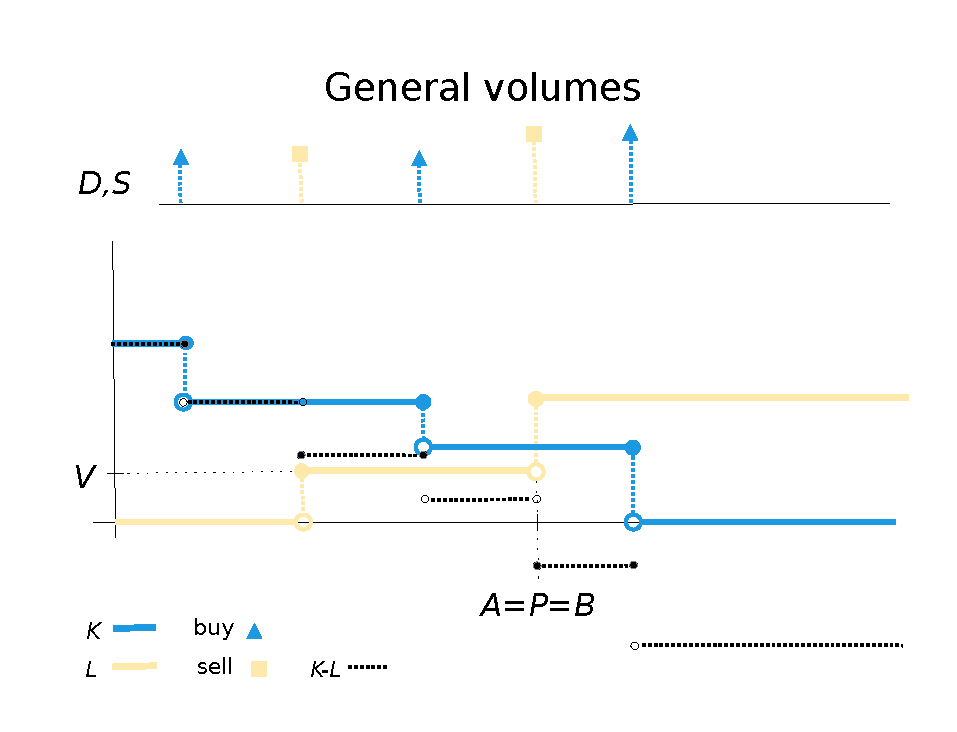
\includegraphics[width=6cm]{nuob.pdf}
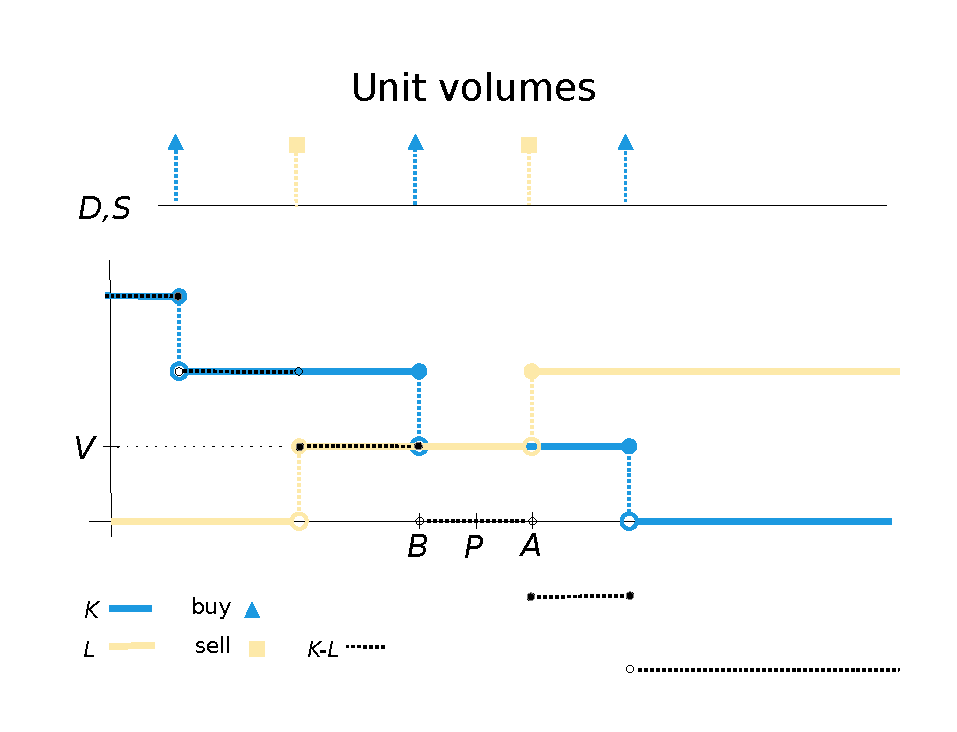
\includegraphics[width=6cm]{ob.pdf}
\end{center}
\caption{Call auction with general order volumes (left) and unit order volumes (right), respectively.}
\label{fig:ob}
\end{figure}

Formally, denoting $K(\pi)=D[\pi,d)$ and $L(\pi)=S(c,\pi]$, $\pi\in I$,
(the demand/supply curves), the maximum traded volume is 
\begin{equation}
V = \max_{p \in I} V^-(p),\qquad V^-(p) \defined K(p) \wedge L(p),
\label{eq:vdef}
\end{equation}
and, further denoting $A=\inf\{\pi\in I:K(\pi)<L(\pi)\}$ and $B=\sup\{\pi\in I:K(\pi)>L(\pi)\}$ 
the price limits,
the clearing price is 
$$P=\begin{cases}\frac{B+A}{2} & A \neq d, B \neq c,
\\\undef & \text{otherwise},
\end{cases}
$$
where $\undef\notin\R$ denotes an undefined price (note, however, that, in some cases with $V=0$, $P$ might be defined). See Figure \ref{fig:ob} for an illustration. 

Our setting covers both the case of continuous limit prices (atoms of $D$ and $S$ may find themselves anywhere in $I$) and the case of discrete prices (atoms of $D$ and $S$ can find themselves only in discrete points, corresponding to price ticks). Note that we do not require the weights (volumes) to be integers. 

Next, we show that $P$ indeed maximizes the traded volume, and, as the traded volume is generally difficult to handle, we introduce its bounds.

\begin{proposition}
(i) 
$$V=\begin{cases} V^-(P) & A \neq d, B \neq c
\\0 & \text{otherwise}
\end{cases}
$$
(ii) For any $p\in I$, $V^-(p) \leq V \leq V^+(p)$ where $V^+(p) = K(p) \vee L(p)$.
\end{proposition}

\begin{proof} (i) When $A = d$ or $B=c$, the assertion is trivial. Let $A \neq d, B \neq c$.
First, note that $V^- = L$ on $(c,A)$ and $V^- = K$ on $(B,d)$. 

Thus, once $B<A$, $V^-$ is non-decreasing on $(c,A)$ and non-increasing on $(B,d)$, which implies that it is constant on $(B,A)$ and  its maximum happens (also on) $(B,A)$, specially in $P$.


If $A=B=P$, then, due to monotonicity, at least one of the following values is equal to $\sup V^-$: $V^-(P-)[=L(P-)],V^-(P+)[=K(P+)]$ or 
$V^-(P)[=K(P) \wedge L(P)=K(P-) \wedge L(P+)]$.
If $K(P-) \geq L(P+)$, then $V^-(P)=L(P+)\geq L(P-)=V^-(P-)$, so only two candidates remain: $V^-(P)[=L(P+)]$ and  $V^-(P+)[=K(P+)]$; however, as the former is strictly greater from the definition of $A$, we proved that the maximum occurs at $P$. Analogously, we can show that $V^-$ is maximized in $P$ if $K(P-) \leq L(P+)$.

\noindent (ii) The first inequality follows directly from (\ref{eq:vdef}). The second one holds trivially if $K(p)=L(p)$ or $V=0$. If $V > 0$ and $K(p)<L(p)$, then $c < B \leq A < p$ hence $P < p$ and, by (i), $V=V^-(P)=K(P) \wedge L(P) \leq L(P) \leq L(p) \leq L(p) \vee K(p)$; similarly for $K(p)>L(p)$.
\end{proof}



\noindent Next we present general formulas for the distribution of random vector $(A,B)$. 

\begin{proposition} \label{th:gen} Let $c<b\leq a \leq d$, put $N_\pi \defined D[\pi,d)-S(c,\pi)$, $\pi \in I$. Then\\
(i) $\P[B<b] = \P[N_b \leq 0]$,\\
(ii)  $\P[A<a] = \P[N_a < 0]$,\\
(iii) $\P[B<b,A<a]=\P[N_b\leq 0]-\P[D[a,d)=S(c,b),S[b,a)=0,D[b,a)=0].$\\
\end{proposition}

\begin{proof} Denote $\Delta = K-L$. As $\Delta$ is a non-decreasing step function, we have
$$[B<b] = [\sup\{\pi\in I:\Delta(\pi)>0\} < b] = [\Delta(b-)\leq 0]$$
and
$$
[A<a] = [\inf\{\pi\in I:\Delta(\pi)< 0 \} < a]
= [\Delta(a-)< 0] 
$$
which proves (i), (ii), respectively because $N_\pi=\Delta(\pi-)$, $\pi \in I$. Further,
\begin{multline*} 
[B<b,A<a] = [\Delta(b-)\leq 0,\Delta(a-)< 0] = [\Delta(b-) < 0] \cup [\Delta(b-) = 0, \Delta(a-)-\Delta(b-) < 0]
\\
=[\Delta(b-) < 0] \cup ( [\Delta(b-) = 0] \setminus E)
\qquad E \defined [\Delta(b-) = 0,\Delta(a-)-\Delta(b-) = 0].
\end{multline*}
As the union is discrete and the difference is proper, we have
$$
\P[B<b,A<a] = \P[\Delta(b-)\leq 0]-\P E = \P[N_b\leq 0]-\P E.
$$
Employing the monotonicity of $\Delta$ and the fact that it jumps at any atom of $D$ or $S$,  we further get
$$
E = [\underbrace{\Delta(b-)}_{=D[b,d)-S(c,b)}=0,S[b,a) = 0, D[b,a)=0], 
$$
which is equivalent to
$$
E=[D[a,d)=S(c,b),S[b,a)=0,D[b,a)=0]
$$
proving (iii).
\end{proof}


\noindent If the offered/ordered volumes are always unit and the atoms of $D$ and $S$ do not coincide w.p.1, then  $K-L$ has unit jumps (down) w.p.1, implying that $B < A$ and, consequently, $V=K(P)=L(P)$ whenever $P\neq \undef$ (note that $V=0$ if $P=\undef$), so we are able to evaluate the joint distribution of $(A,B,V)$:

\begin{proposition} \label{th:general} Let the atoms of $D+S$ have unit weights w.p.1. Then, for any $c< b \leq a < d$ and any $X \subseteq \N_0$,
\begin{equation}
\P[B<b,A>a,V\in X]=\P[ D[b,a] = 0, S[b,a] = 0, D(a,d)=S(c,b)\in X].
\label{eq:pbax}
\end{equation}
\end{proposition}

\begin{proof} Denote $p = \frac{a+b}2$. As $\Delta \defined K-L$ is non-increasing, we have
\begin{multline*}
[B < b,A > a] = [\sup\{\pi\in I:\Delta(\pi)>0\} < b \leq a < \inf\{\pi\in I:\Delta(\pi)< 0 \} ]
\\= [\Delta(b-)\leq 0,\Delta(a+)\geq 0] = [\Delta(b-) = 0,\Delta(a+) = 0]
= [\Delta(b-)=0, \Delta(b-)-\Delta(a+)=0]
\\=[D[b,d)=S(c,b), D[b,a] = 0, S[b,a] = 0]
=[ D(a,d)=S(c,b), D[b,a] = 0, S[b,a] = 0].
\end{multline*}
Therefore and as $B<b,A>a \Rightarrow V=D(a,d)=S(c,b)$, we get (\ref{eq:pbax}).

\end{proof}



\section{Completely Random Order Books}
\label{sec:cr}

Next, we discuss the special case where $D$ and $S$ are mutually independent and completely random. Recall that a random measure $M$ on $(I, \B(I))$ is {\em completely random} if, for any disjoint $S_1,\dots,S_k\in \B(I)$, $MS_1,\dots,MS_k$ are independent. Note also that the class of completely random measures embraces (marked) diffuse Poisson point processes (viewed as measures) as well as the measures with fixed atoms with mutually independent weights (usable in discrete price settings). In fact, any completely random purely atomic measure is a sum of a measure of the former type and a measure of the latter type (see \cite{daley03}, Theorem 10.1.III). 

It is well known (see, e.g. \cite{daley03}, 2.1.6 and 10.1.VI) that a measure $M=\sum_{i=1}^N W_i \delta_{U_i}$, where $\delta_x$ is the Dirac measure concentrated in $x$, $N$ is Poisson, $U_i$'s are i.i.d,, $W_i$'s are i.i.d. and $N,U_1,W_1,U_2,\dots$ are mutually independent (the setting studied by \cite{toke2015exact}) is completely random, but stops to be so once $N$ becomes deterministic (which is the case studied by \cite{derksen2020clearing}); consider $M=\delta_U$ with random $U$, for instance. Further note that, once the process of order arrivals is Poisson and the orders are possibly canceled with a fixed rate, dependent only on the limit price, then the process of valid orders is still Poisson and the corresponding order book is still completely random and Poisson (see, e.g. \cite{smid16estimation}, Example 2.3).


The following result stems directly from Proposition \ref{th:gen}:

\begin{proposition}
\label{cor:cr} If $D \indep S$ and both $D$ and $S$ are completely random, then, for any $c < b \leq a \leq d$,
$$\P[B<b,A<a] = \P[N_b\leq 0]-\P[D[a,d)=S(c,b)]\P[S[b,a)=0]\P[D[b,a)=0]$$
\end{proposition}

\begin{example} Assume discrete prices: $c=0$, $d \in \N$, $D=\sum_{i=1}^{d-1} \delta_i V_i$, 
$S=\sum_{i=1}^{d-1} \delta_i W_i$ where $V_i \sim \mathrm{Bernoulli}(\pi)$, $W_i \sim \mathrm{Bernoulli}(\pi)$, $0 < i < d$, with $V_1,W_1,V_2,\dots,W_{d-1}$ independent. Then
$$
\P[A=d]=\P[B=c]=(1-\pi)^{d-1}, \qquad  \P[A=d, B=c]=(1-\pi)^{2d-2},
$$
and, by Proposition \ref{cor:cr}, for any $0 < a \leq b < d$,
\begin{multline*}
\P[B< b, A < a]
%\\ = \P[D[b,d)-S(c,b)\leq 0]-\P[D[a,d)=S(c,b)] \P[S[b,a)=0]\P[D[b,a)=0]
=
\P[\Bi(d-b,\pi)\stackrel{\indep{}}-\Bi(b-1,\pi)\leq 0] \\ -\P[\Bi(d-a,\pi)\stackrel{\indep{}}-\Bi(b-1,\pi)=0]
\P[\Bi(a-b,\pi)=0]\P[\Bi(a-b,\pi)=0] \\
= \sum_{k=-(b-1)}^0 q_{d-b,b-1,\pi}(k)-q_{d-a,b-1,\pi}(0)(1-\pi)^{2a-2b}
\end{multline*}
where $q_{m,n,\pi}(k) \defined \P[\Bi(m,\pi)\stackrel{\indep{}}-\Bi(n,\pi)=k]$ for any $m,n,\pi,k$. Using this and the fact that $\P[B>A]=0$ we can obtain the distribution of $(A,B)$. In Figure \ref{fig:bin}, this distribution is plotted for $d=11$ and various values of $\pi$.
\end{example}

\begin{figure}
\begin{center}
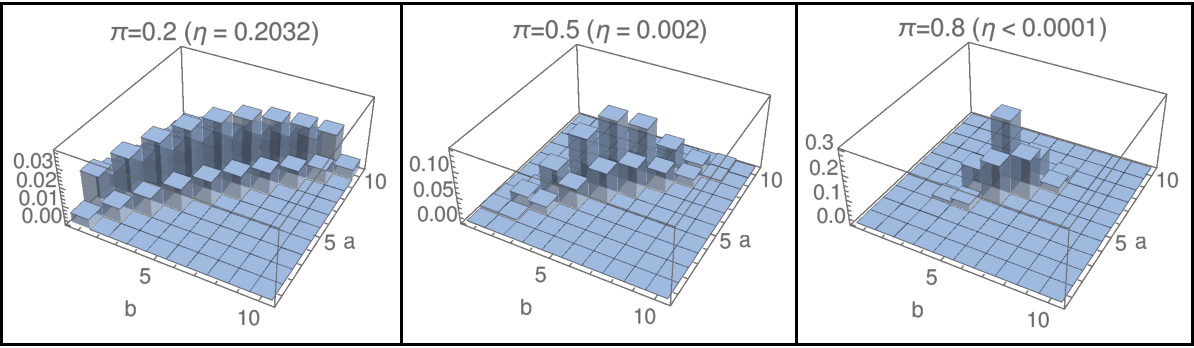
\includegraphics[width=\textwidth]{binom.pdf}
\caption{Distribution of $(A,B)$ in a call auction with $c=0$, $d = 11$, $D=\sum_{i=1}^{d-1} \delta_i V_i$, 
$S=\sum_{i=1}^{d-1} \delta_i W_i$, $V_i \sim \mathrm{Bernoulli}(\pi)$, $W_i \sim \mathrm{Bernoulli}(\pi)$, $0 < i < d$, $\indep(V_1,W_1,V_2,\dots,W_{d-1})$, for various levels of $\pi$. Here, $\eta = \P[B = 0 \vee C = 11]$.}
\label{fig:bin}
\end{center}
\end{figure}


\section{Unit Order Volumes}
\label{sec:cru}

In this subsection, we keep assuming $D\indep S$ to be completely random, but study the special case of the $D$ and $S$ being diffuse (i.e. for any $x\in I$, $D\{x\}=0$, $S\{x\}=0$ w.p.1) and simple (the atoms' weight is always unit). Given these assumptions, by \cite{Kallenberg02}, Theorem 12.10, both $D$ and $S$ are (equivalent to simple) Poisson point processes. Note that, due to our assumption of a finite number of atoms, $D$ and $S$ are fully characterized by 
$\kappa(x)\defined \E K(x)$, $\lambda(x)\defined\E L(x)$, respectively, $x \in I$, with $\kappa(c+)<\infty,\lambda(d-) < \infty$. Let us also recall that we can represent $D=\sum_{i=1}^{N_D} \delta_{V_i}$ where ${N_D}\sim \Po(\kappa(c+))$, the c.d.f. of each $V_i$, $i\in \N$, is $F_D(\bullet)\defined 1-\kappa(\bullet)/\kappa(c+)$, with $\indep (N_D.V_1,V_2,\dots)$ and, similarly, $S=\sum_{i=1}^{N_S} \delta_{W_i}$ where ${N_S}\sim \Po(\lambda(d-))$, the c.d.f. of each $W_i$ is $F_S(\bullet)=\lambda(\bullet)/\lambda(d-)$, and $\indep (N_S.W_1,W_2,\dots)$. 

The following result is a direct consequence of Proposition \ref{th:general}:

\begin{proposition} If $D \indep S$ are (simple) diffuse Poisson, then, for any $c < b \leq a < d$ and $X \subset \N_0$,
\begin{multline}
\P[B<b,A>a,V\in X]=\P[ D[b,a] = 0 ]\P[ S[b,a] = 0]\P[D(a,d)=S(c,b)\in X]\\
= e^{-(\lambda(a)-\lambda(b))}e^{-(\kappa(b)-\kappa(a))}\P[D(a,d)=S(c,b)\in X].
\label{eq:pax}
\end{multline}
\end{proposition}

Applying (\ref{eq:pax}) to single-element $X$'s, we get:
\begin{corollary} For any $c < b \leq a < d$, and $i \in \N_0$,
\begin{multline}
\P[B<b,A>a,V = i] = p(b,a,\{i\}) \\ \defined e^{-(\lambda(a)-\lambda(b))}e^{-(\kappa(b)-\kappa(a))} e^{-\kappa(a)} \frac{\kappa(a)^i}{i!}e^{-\lambda(b)} \frac{\lambda(b)^i}{i!}
 = e^{-\kappa(b)-\lambda(a)} \frac{\kappa(a)^i}{i!}\frac{\lambda(b)^i}{i!}.
\label{eq:pbai}
\end{multline}
\end{corollary}
Further, by taking $X = \N_0$ and using the fact that, for any $\mu\geq 0$ and $\nu \geq 0$, $\P[\Po(\mu)\stackrel{\indep{}}{-}\Po(\nu)=0]=e^{-\mu-\nu}I_{0}(2\sqrt{\mu\nu})$ where $I_0$ is the zero-order modified Bessel function of the first kind (see e.g. \cite{skellam1946frequency}), we get:
\begin{corollary} For any $c < b\leq a < c$,
\begin{equation}
\P[B<b,A>a]=p(b,a,\N_0) \defined e^{-\kappa(b)-\lambda(a)} I_{0}(2\sqrt{\kappa(a)\lambda(b)}).
\label{eq:pba}
\end{equation}
\end{corollary}
\begin{remark}
Equivalently, we can sum (\ref{eq:pbai}) to get,
$$
p(b,a,\N_0)=e^{-\kappa(b)-\lambda(a)}\sum_{i=0}^\infty\frac{(\kappa(a)\lambda(b))^i}{i!i!}.
$$
\end{remark}
As $\P[B\geq A]=0$, (\ref{eq:pbai}) and (\ref{eq:pba}) suffice to evaluate the distributions of $(A,B,V)$, $(A,B)$, respectively.

Assume, until the end of this Section, that $\kappa$ and $\lambda$ are differentiable.

\begin{proposition}
\label{th:abv}
Let either $X = \N_0$ or $X = \{i\}$ for some $i\in \N_0$. Then, for any $Q\in\B([c,d)\times(c,d])$,
\begin{multline}
\P[(B,A,V)\in Q \times X]=\int_{\{(b,a)\in Q: c<b<a<d\}}\gamma(b,a,X)dadb\\
+\charf [0\in X] \left[\int_{\{a:(c,a) \in Q \}}\alpha(a)da
+\int_{\{b:(b,d) \in Q \}}\beta(b)db+\charf[(c,d)\in Q]e^{-\kappa(c)-\lambda(d)}
\right],
\label{eq:pbc}
\end{multline}
where 
$$
\alpha(a)\defined 
\lambda'(a)e^{-\kappa(c)-\lambda(a)},\qquad
\beta(b)\defined-\kappa'(b)e^{-\kappa(b)}{}^{-\lambda(d)},
$$
and
$$
\gamma(b,a,X) = -\frac{\partial}{\partial a\partial b}p(b,a,X).
$$
\end{proposition}

\begin{proof}
See Appendix \ref{app:abv}.
\end{proof}

\begin{corollary}\label{cor:abdens} For any $Q\in\B([c,d)\times(c,d])$,
\begin{multline*}
\P[(B,A)\in Q]=\int_{\{(b,a)\in Q, b \in I, a \in I\}}g(b,a)dadb\\
+\int_{\{a:(c,a) \in Q \}}\alpha(a)da
+\int_{\{b:(b,d) \in Q \}}\beta(b)db+\charf[(c,d)\in Q]e^{-\kappa(c)-\lambda(d)}
\end{multline*}
where 
$$g(b,a)=0,\qquad a<b, $$
and
\begin{multline}
g(b,a)
%= e^{-\kappa(b)-\lambda(a)}
%\left(
%-\kappa'(b)\lambda'(a) \sum_{i=0}^\infty \frac{\lambda(b)^i\kappa(a)^i}{i!i!}
%+\kappa'(a)\kappa'(b) \sum_{i=0}^\infty \frac{\lambda(b)^{i+1}\kappa(a)^i}{(i+1)!i!}
%\right.
%\\
%\left.
%+\lambda'(b)\lambda'(a) \sum_{i=0}^\infty \frac{\lambda(b)^{i}\kappa(a)^{i+1}}{(i+1)!i!}
%-\lambda'(b)\kappa'(a) \sum_{i=0}^\infty \frac{\lambda(b)^{i}\kappa(a)^{i}}{i!i!}
%\right)\\
= e^{-\kappa(b)-\lambda(a)}
\left(
-\left[\kappa'(b)\lambda'(a)+\lambda'(b)\kappa'(a)\right] I_0(2\sqrt{\kappa(a)\lambda(b)})
\right.
\\
\left.
+\left[\kappa'(a)\kappa'(b)
\sqrt{\frac{\lambda(b)}{\kappa(a)}}
+\lambda'(a)\lambda'(b)
\sqrt{\frac{\kappa(a)}{\lambda(b)}}\right] I_1(2\sqrt{\kappa(a)\lambda(b)})
\right), \qquad a \geq b,
\label{eq:gamma}
\end{multline}
where $I_k$ is the modified Bessel function of $k$ -th order of the first kind; we take $\kappa'(a)\sqrt{\frac{\lambda(b)}{\kappa(a)}}=0$ whenever $\kappa(a)=0$ and 
$\lambda'(b)
\sqrt{\frac{\kappa(a)}{\lambda(b)}}=0$ whenever $\lambda(b)=0$.
\end{corollary}



\begin{proof} See Appendix \ref{app:abdens}.
\end{proof}

Furthermore, we evaluate the distribution of $(P,V)$:

\begin{proposition}
Let $X \subseteq \N_0$ be as in Proposition \ref{th:abv}. Then, 
\begin{equation}
\P[P=\undef, V\in X]=\charf[0\in X] [e^{-\kappa(c)}+e^{-\lambda(d)}-e^{-\kappa(c)-\lambda(d)}]\label{eq:pd0}
\end{equation}
and, for any $p\in I$,
\begin{multline}
\P[P<p,P\neq\undef,V\in X]\\=
%\Phi_{\kappa,\lambda}(p)\defined
\int_{c}^{p}\eta(a,a,X)da+\int_{p}^{(2p-c) \wedge d}\eta(2p-a,a,X)da+\charf[0 \in X] [e^{-\kappa(c)-\lambda((2p-c) \wedge d)}-e^{-\kappa(c)}]
\label{eq:pdist}
\end{multline}
where $\eta(b,a,X)=-\frac{\partial}{\partial a} p(b,a,X)$, $b<a$. 
\end{proposition}

\begin{proof}
By Proposition \ref{th:abv}, 
\begin{multline*}
\P[P<p,P\neq\undef,V\in X] =\P[A<d,c<B<2p-A,V\in X]
\\ =\int_{\{a < d\}}\int_{\{ c < b < 2p-a\}}\P_{(B,A,V)}(db,da,X)\\
=\int_{\{c< a < d\}}\int_{\underbrace{\{ c < b < 2p-a, b < a \}}_{\text{$=\emptyset$ for $a \geq 2p-c$}}}\gamma(b,a,X)dbda\\
=\int_c^{(2p-c) \wedge d}\int_c^{a \wedge (2p-a)} \gamma(b,a,X)dbda \\
=\int_c^{(2p-c) \wedge d}[ \eta(a \wedge 2p-a,a,X)da - \eta(c,a,X)]da\\
=\underbrace{\int_c^{(2p-c) \wedge d} \eta(a \wedge 2p-a,a,X)da}_
{=\int_c^p \eta(a, {\dots} + \int_p^{(2p-c) \wedge d} \eta(2p-a,\dots} +
\underbrace{\left[p(c,(2p-c) \wedge d,X)-p(c,c,X)\right]}_{=\charf[0\in X](e^{-\kappa(c)-\lambda((2p-c) \wedge d)}-e^{-\kappa(c)})}
\end{multline*}
(see Appendix \ref{app:abv} for the definition of $p(c,\bullet,X)$).
\end{proof}

\begin{theorem}
(i)
$$
\P[P=\undef]=e^{-\kappa(c)}+e^{-\lambda(d)}-e^{-\kappa(c)-\lambda(d)}.
$$

\noindent (ii) For any $p\in I$ and $v \in \N_0$,
\begin{multline}
\P[P<p,P\neq\undef,V = v]=
%\Phi_{\kappa,\lambda}(p)\defined
\int_{c}^{p}\psi(a,a,v)da \\ +\int_{p}^{(2p-c) \wedge d}\psi(2p-a,a,v)da+\charf[v=0] (e^{-\kappa(c)-\lambda((2p-c) \wedge d)}-e^{-\kappa(c)}),
\label{eq:pdist2}
\end{multline}
where
$$
\psi(b,a,v)=
\begin{cases}
e^{-\kappa(b)-\lambda(a)}\lambda'(a) & v=0,\\
e^{-\kappa(b)-\lambda(a)}\frac{\lambda(b)^v}{v!}\left(\lambda'(a)\frac{\kappa(a)^v}{v!}
- \kappa'(a)\frac{\kappa(a)^{v-1}}{{(v-1)}!}\right) & v>0.
\end{cases}
$$
\noindent (iii) For any $p \in I$,
\begin{multline}
\P[P<p,P\neq\undef]\\=
%\Phi_{\kappa,\lambda}(p)\defined
\int_{c}^{p}\phi(a,a)da+\int_{p}^{2p \wedge d}\phi(2p-a,a)da + [e^{-\kappa(c)-\lambda(2p \wedge d)}-e^{\kappa(c)}],
\label{eq:ppu}
\end{multline}
where 
$$
\phi(b,a)=
e^{-\kappa(b)-\lambda(a)}\left(-\lambda'(a)I_0(2\sqrt{\kappa(a)\lambda(b)})+\kappa'(a)\sqrt{\frac{\lambda(b)}{\kappa(a)}}I_1(2\sqrt{\kappa(a)\lambda(b)})\right)
$$
taking $\kappa'(a)\sqrt{\frac{\lambda(b)}{\kappa(a)}}=0$ whenever $\kappa(a)=0$.

\noindent (iv) For any $v\in \N_0$,
$$
\P[V=v]\\=
%\Phi_{\kappa,\lambda}(p)\defined
\int_{c}^{d}\psi(a,a,v)da + \charf[v = 0] e^{-\lambda(d)}.
$$
\end{theorem}

\begin{proof} (i) follows from (\ref{eq:pd0}), (ii) and (iii) follow from (\ref{eq:pdist}), to get (iv), it suffices to take the limit $p\rightarrow d$ in (\ref{eq:pdist}).
\end{proof}

\begin{corollary} \label{cor:dens}
 $P$ is absolutely continuous w.r.t. $\delta_\undef+\ell((c,d))$, where $\ell$ denotes the Lebesgue measure, with density 
\begin{equation}
f(\undef)=e^{-\kappa(c)}+e^{-\lambda(d)}-e^{-\kappa(c)-\lambda(d)},\qquad 
f(p)=2 \int_p^{2 p \wedge d} g(2p-a,a) da.
\label{eq:pdens}
\end{equation}
\end{corollary}

\begin{proof} See Appendix \ref{app:dens}.
\end{proof}




 

\section{Random Order Volumes}
\label{sec:crr}

In the present Section, we release the assumption of unit weights, still assuming that $D\indep S$ are diffuse complete random, but allowing for (i.i.d.) random weights with the same distribution for buy-- and the sell orders. Under these assumptions, the locations of the $D$'s and $S$'s atoms form a (diffuse) Poisson point processes, which we denote $D_g$, $S_g$, respectively.

\def\cpo{\mathrm{CPo}}

\begin{theorem} Let $D \indep S$, let $D_g$, $S_g$ be diffuse Poisson and let the weights of the atoms be i.i.d., following a distribution $\L$ such that $\L(-\infty,0]=0$. Then, for any $c < b \leq a < d$,
\begin{equation}
\label{eq:pbcp}
\P[B<b] = \P[\mathcal{C}(\kappa_g(b),\lambda_g(b),\L)\leq 0],
\end{equation}
\begin{equation}
\label{eq:pacp}
\P[A<a] = \P[\mathcal{C}(\kappa_g(a),\lambda_g(a),\L)< 0],
\end{equation}
and
\begin{multline*}
\P[B<b,A<a] = \P[\mathcal{C}(\kappa_g(b),\lambda_g(b),\L)\leq 0]
\\
- e^{-(\lambda_g(a)-\lambda_g(b))}e^{-(\kappa_g(b)-\kappa_g(a))}\P[\mathcal{C}(\kappa_g(a),\lambda_g(b),\L)=0];
\end{multline*}
here, $\kappa_g(\pi)=\E D_g[\pi,d)$, $\lambda_g(\pi)=\E S_g(c,\pi]$, $\pi \in I$, and $\mathcal{C}(\kappa,\lambda,\L)$ is the Compound Poisson distribution with intensity $\kappa+\lambda$ and embedded distribution $\frac\kappa{\kappa+\lambda} \L + \frac\lambda{\kappa+\lambda} \L^-$ where $\L^-$ is  the $\L$'s negative version (i.e. $\L(x,\infty)=\L^-(-\infty,-x)$, $x \in \R$).
\end{theorem}
\begin{proof}
The assertion follows from Proposition \ref{cor:cr}, using the fact that the convolution of two compound Poisson distributions is compound Poison with properly weighted mixed embedded distribution.
\end{proof}

%https://www.sciencedirect.com/science/article/abs/pii/0167637784900087

\noindent In the following Theorem, we evaluate the asymptotic distributions of the clearing price and the bounds of the traded volume.

\begin{theorem} \label{th:asymp} Let $\kappa_0,\lambda_0:I\rightarrow \R_+$ be strictly increasing, decreasing, respectively, and differentiable. Let $\L$ be distribution with $\L(-\infty,0]=0$ having a finite third moment. For any $n \in \N$, let $P_n,B_n,A_n,\dots$ be the clearing price, lower price limit, upper price limit, etc., in a call auction with independent compound Poisson order books defined by $\kappa_g = n \kappa_0$ and $\lambda_g = n\lambda_0$ and the atoms' weight distribution $\L$. Let $p$ be the solution of the equation $\kappa_0(p)= \lambda_0(p)$. Then\\
(i) $$P_n\stackrel{P}\longrightarrow p$$
(ii)
\begin{multline*}
\sqrt{n}(P_n-p) \stackrel{d} \longrightarrow \ND\left(0,v_gr_\L\right), 
\\ 
v_g \defined \frac{\kappa_0(p)+\lambda_0(p)}{(\lambda_0'(p)-\kappa_0'(p))^2}=\frac{2\kappa_0(p)}{(\lambda_0'(p)-\kappa_0'(p))^2}
=
\frac{2\lambda_0(p)}{(\lambda_0'(p)-\kappa_0'(p))^2},
\qquad
r_\L = \frac{\E \L^2}{(\E \L)^2},
\end{multline*}
where  $\E\L$ and $\E\L^2$ are the $\L$'s expectation, (non-central) second moment, respectively.\\
(iii) 
$$W^-_n \leq V_n \leq W^+_n,\qquad 
W^-_n \defined V_n^-(p),\qquad W_n^+ \defined V_n^+(p),$$
with
$$
\frac{1}{\sqrt{n}}(W_n^--n \mu)\stackrel{d}\longrightarrow \mathcal{M}_{w}, 
\qquad 
\frac{1}{\sqrt{n}}(W_n^+-n \mu)\stackrel{d}\longrightarrow \mathcal{M}^{w};
$$
$$
\mu = \kappa_0(p) \E\L = \lambda_0(p) \E\L, \quad
w = 
\kappa_0(p) \E \L^2= \lambda_0(p) \E \L^2,
$$
where $\mathcal{M}_w$, $\mathcal{M}^w$, are the distributions of the minimum, maximum, respectively, of two independent $\ND(0,w)$ random variables. In particular
$$
\P\left[ \frac{1}{\sqrt{n}}(W^-_n-n \mu)  < x
\right] = 1-\left(1-\varphi\left(\frac{x}{\sqrt{w}}\right) \right)^2,
$$
$$
\P\left[ \frac{1}{\sqrt{n}}(W^+_n-n \mu) < x
\right] = \varphi\left(\frac{x}{\sqrt{w}}\right)^2,
$$
where $\varphi$ is the standard normal c.d.f.
\end{theorem}

\begin{proof} See Appendix \ref{app:asymp}.
\end{proof}


\begin{corollary}
If, in Theorem \ref{th:asymp}, $\L = \delta_1$ (i.e., the volumes are deterministic and unit), then the Theorem holds with 
$v_g = \frac{2\kappa(p)}{[\lambda'(p)-\kappa'(p)]^2}$, $r_L=1$, $\mu = w = \kappa(p)=\lambda(p)$.
\end{corollary}

\paragraph*{Numerical Illustration.}
Once the trading intensities are high enough, we can represent $P=P_n$, $V^-(p)=V_n^-(p)$ and $V^+(p)=V_n^+(p)$ for some $n$ and approximate
$$
P \quad \dot \sim \quad 
\ND\left(p,\frac{2\kappa_g(p)\E\L^2}{(\kappa'_g(p)-\lambda'_g(p))^2(\E \L)^2} \right ),
$$
and
$$
W^- \leq V \leq W^+,
$$
where
$$
\P\left[ W^-  < x
\right] \doteq 1-\left(1-\varphi\left(\frac{\kappa_g(p)\E \L+x}{\sqrt{\kappa_g(p)\E \L^2}}\right) \right)^2
$$
$$
\P\left[ W^+ < x
\right] \doteq \varphi\left(\frac{\kappa_g(p)\E \L+x}{\sqrt{\kappa_g(p)\E \L^2}}\right)^2
$$
$x \in I$. In Figure \ref{fig:il}, we illustrate the accuracy of these approximations for various levels of trading intensity: we assume that order volumes and intensities are multiples of linear functions, different for demand and supply. It can be seen that the approximations are nearly perfect, once there are tens of orders on both sides (recall that the expected number of buy and sell orders equals $\kappa(c+)$, $\lambda(d-)$, respectively.

\begin{remark} As, by the Schwarz inequality, $r_\L \geq 1$, with the minimum achieved by $\L = \delta_1$, we see that taking randomness of the order volumes into account leads to higher (asymptotic) variance of both the price and the volume bounds in comparison with the usual approximation of the volumes by their mean values (normed to one). 
\end{remark}

Next, we compare our asymptotic result with that of \cite{derksen2020clearing}:

\begin{remark} Consider
$$
D=\sum_{i=1}^{N_D} \delta_{D_i}, \qquad S=\sum_{i=1}^{N_S} \delta_{S_i}
$$
where $\E N_D=(1-\alpha)n$, $\E N_S=\alpha n$ for some $\alpha \in (0,1)$ and $n\in \N$,  $D_i$, $i\in\N$, being i.i.d. with strictly increasing absolutely continuous c.d.f. $F_D$, and $S_i$, $i\in \N$ being i.i.d. with strictly increasing a.c. c.d.f $F_S$, such that all the variables are mutually independent.

Once $N_S$ and $N_D$ are Poisson, $D$ and $S$ are Poisson processes determined by 
$$
\kappa(x)=n (1-\alpha) (1-F_D(x)), \qquad \lambda(x)=n \alpha F_S(x),
$$
and, by Theorem \ref{th:asymp},
$$
\sqrt{n}(P_n-p) \rightarrow_n \ND(0,v), 
\qquad 
v=\frac{ 2 \alpha F_S(p) }{[(1-\alpha)f_D(p)+\alpha f_S(p)]^2}.
$$
 

If, instead, $N_D=(1-\alpha) n$ and $N_S = \alpha n$ are deterministic, we have, by Theorem 3.1 of \cite{derksen2020clearing}, that 
$$
\sqrt{n}(P_n-p) \rightarrow_n \ND(0,\tilde v), 
\qquad 
\tilde v=\frac{ \alpha [F_D(p)+ (1-F_S(p))]F_S(p)}{[(1-\alpha)f_D(p)+\alpha f_S(p)]^2}
$$
By comparison of the asymptotic variances we see that assuming random order numbers increases the price variance significantly compared with only using their expectations. 
\end{remark}


\begin{figure}
\begin{center}
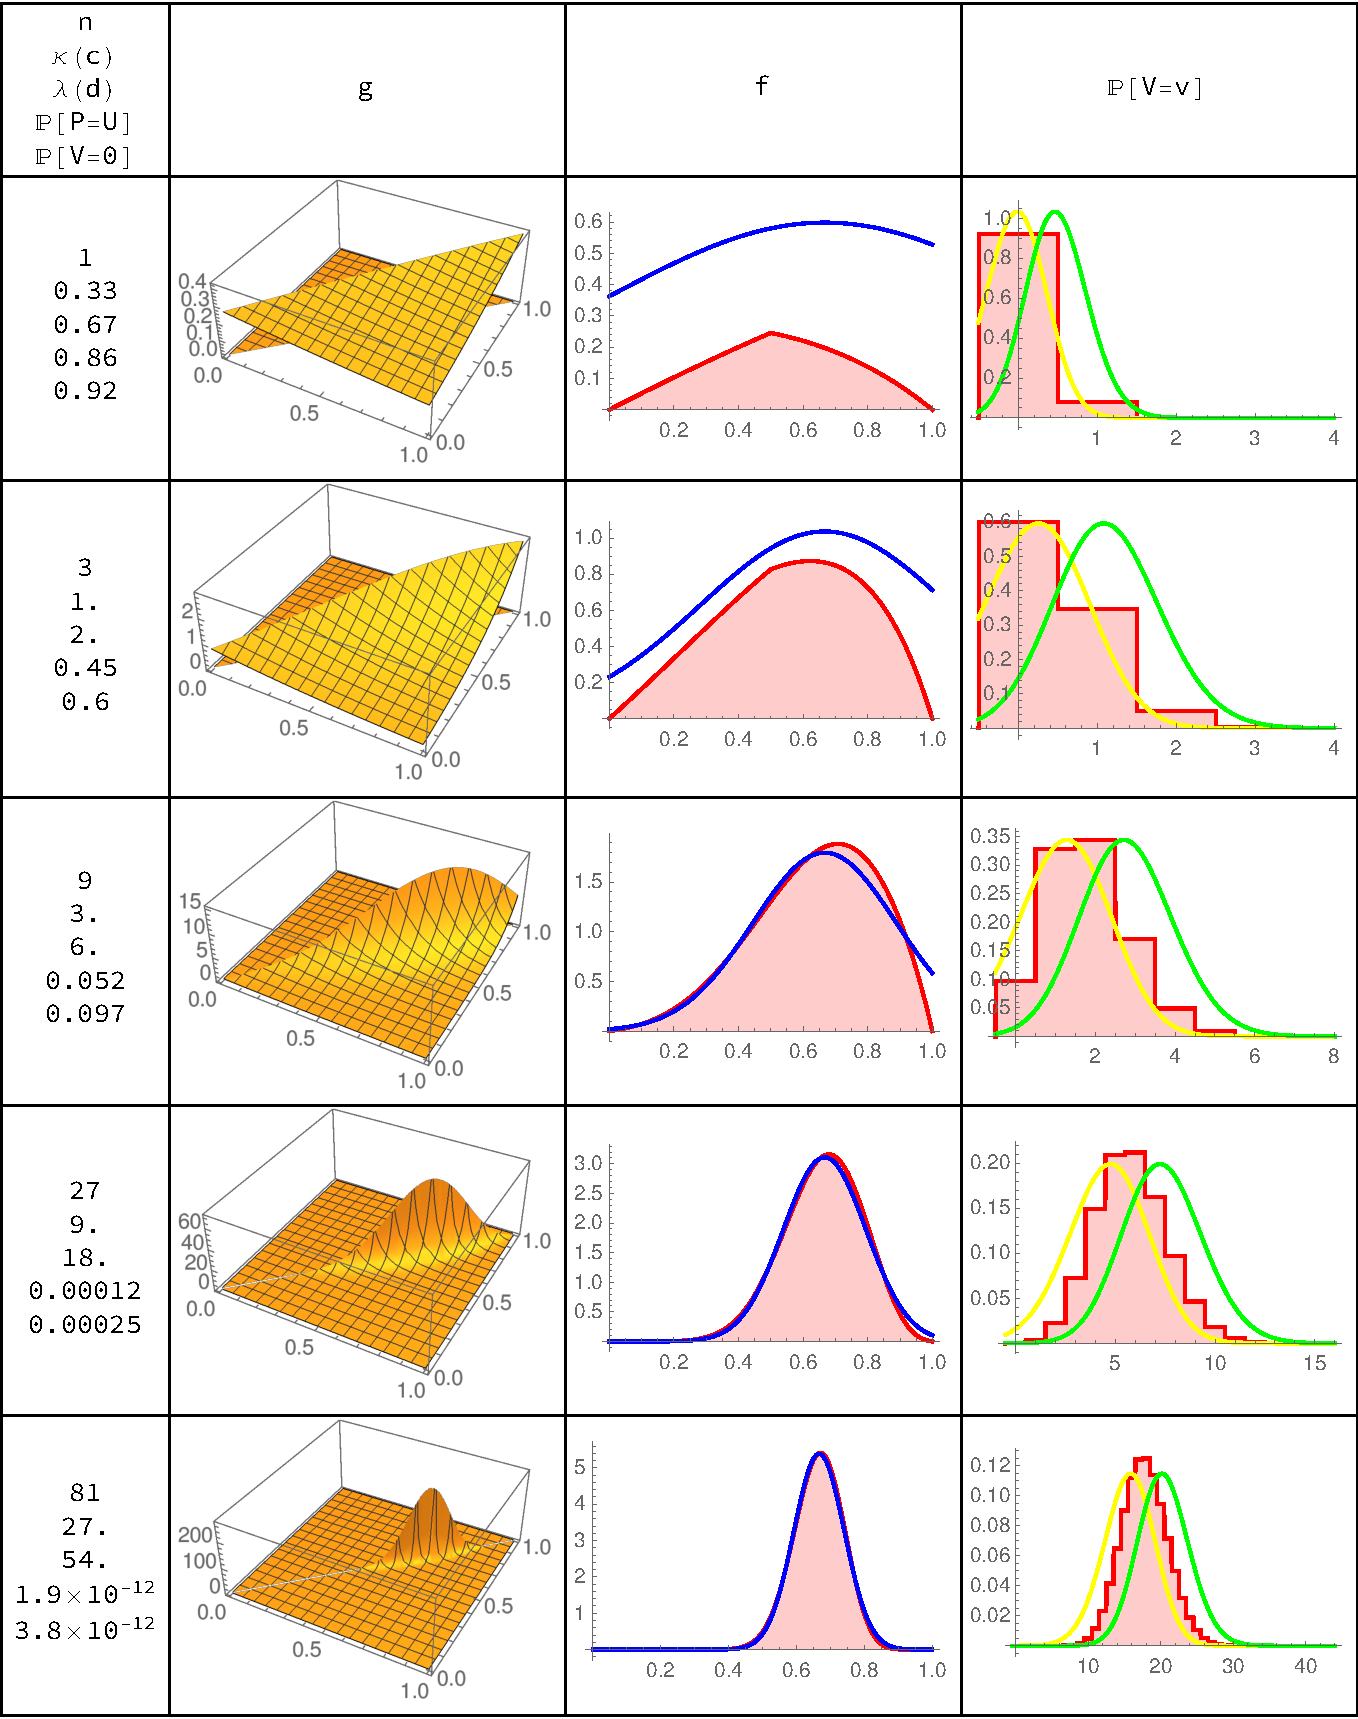
\includegraphics[width=\textwidth]{illust.pdf}
\caption{Distribution of $(A,B)$, $P$ and $V$ for $\kappa(a)=n \frac{2}{3}(1-a)$, $\lambda(b)=n \frac{1}3 b$ and unit order volumes. Blue, normal approximation of $P$, yellow, normal approximation of $W^-$, green, normal approximation of $W^+$. }
\label{fig:il}
\end{center}
\end{figure}

\section{Conclusions}

We have thoroughly studied a natural stochastic model of call auction. We have described both the exact and the asymptotic distributions in various special cases of this model. The next natural step could be to describe the dynamics of repeated call auctions, suggested by \cite{budish2015high}, and compare it with that of the continuous double auction.

\paragraph*{Acknowledgments} This work was supported by grant No. GA19-11062S from the Czech Science Foundation. Computational resources were partially provided by the ``eInfrastruktura CZ'' (e-INFRA CZ LM2018140) project supported by the Ministry of Education, Youth and
Sports of the Czech Republic

%\bibliographystyle{APT}
\footnotesize
%\bibliography{../../smid}
\documentclass{aptpub}
\usepackage{graphicx}
\usepackage{hyperref}
\authornames{\v Sm\'\i d, Kub\v ena} % insert the authors here for use in running head. If three or more authors please use (for example) M.~YARROW {\it et al}. Author names should follow the same M.~YARROW format and if two authors, separate by 'AND'.
\shorttitle{Distribution of Call Auction} % insert short title here for use in running head

% Put any of your own definitions here.

%\numberwithin{equation}{section}  % If you number theorems, etc. within sections,
                                   % then please uncomment this line to number
                                   % equations with sections too.

\global\long\def\P{\mathbb{P}}%
\global\long\def\N{\mathbb{N}}%
\global\long\def\U{\mathbb{U}}%
\global\long\def\E{\mathbb{E}}%
\global\long\def\R{\mathbb{R}}%
\global\long\def\G{\mathcal{G}}%
\global\long\def\g{\mathbb{\Pi}}%
\global\long\def\F{\mathcal{F}}%
\global\long\def\S{\mathbb{S}}%
\global\long\def\Q{\mathcal{Q}}%
\global\long\def\B{\mathcal{B}}%
\global\long\def\ND{\mathcal{N}}%
\global\long\def\XX{\mathcal{X}}%
\global\long\def\indep#1{{\perp\hspace{-2mm}\perp}#1}%
\global\long\def\L{\mathcal{L}}%
\global\long\def\var{\mathrm{var}}%
\global\long\def\cov{\mathrm{cov}}%
\global\long\def\charf{\mathbf{1}}%
\global\long\def\d{\mathrm{d}}%
\global\long\def\M{\mathcal{M}}%
\global\long\def\Exp{\mathrm{Exp}}%
\global\long\def\Uniform{\mathrm{U}}%
\global\long\def\eqd{\stackrel{d}{=}}%
\global\long\def\eqas{\stackrel{a.s.}{=}}%
\global\long\def\X{\mathcal{X}}%
\global\long\def\supp{\mathrm{support}}%
\global\long\def\H{\mathcal{H}}%
\global\long\def\Z{\mathcal{Z}}%
\global\long\def\as{\qquad a.s.}%
\global\long\def\on{\qquad\text{on }}%
\global\long\def\C{\mathcal{C}}%
\global\long\def\barxi{\overline{\xi}}%
\global\long\def\Po{\mathrm{Po}}%
\global\long\def\Bi{\mathrm{Bi}}%
\global\long\def\Be{\mathrm{Be}}%
\global\long\def\defined{\stackrel{\text{def}}{=}}%
\global\long\def\barA{\overline{A}}%
\global\long\def\A{\mathcal{A}}%
\global\long\def\barx{x}%
\global\long\def\barX{TBD}%
\global\long\def\last{\ell}%
\global\long\def\bary{y}%
\global\long\def\barz{z}%
\global\long\def\DD{\mathcal{D}}%
\global\long\def\undef{\mathfrak{U}}


\begin{document}%\recd{}{}%Do not alter this line.

\title{Distribution of Price and Volume in Call Auction} % insert title - use `\\ if it requires more than one line.

\authorone[Czech Academy of Sciences]{Martin   \v Sm\'\i d} 
%Affiliation is just the name of your university or institution, for example 'University of Sheffield'. Author names should be of the form 'Mark Yarrow'. 
%Authors should be ordered alphabetically subject to the convention in that particular authors country. For example 'Remco van der Hofstad' would be listed under 'H' as is standard in the Netherlands. 
\authortwo[Czech Academy of Sciences]{Ale\v s Anton\`\i n Kub\v ena} 

%Please use the following format for addresses and emails. The APT office will sort this out after you submit your files.
\addressone{Institute of Information Theory and Automation of the CAS. Pod Vod\' arenskou v\v e\v z\'\i 4, Praha 8, 182 00, Czech Republic,
              Tel.: +420-2-66052400} % Your postal address goes here.
\emailone{smid@utia.cas.cz} %Authors email goes here.

\begin{abstract}

We describe exact and asymptotic distributions of the settlement price and the traded volume in call auction. On top of existing results, we allow completely random order books and random order volumes. We show that approximating random order volumes and/or order numbers by constants leads to a significant underestimation of both the settlement price and the traded volume variances. We also demonstrate a rapid speed of convergence of the asymptotic distributions to the exact ones. 
%, which is a trading mechanism accumulating demand and supply for some time period and then settling them for a price maximizing the traded volume. 

\end{abstract}

\keywords{call auction, settlement price, traded volume, exact distribution, asymptotic distribution}%insert keywords separated by a semicolon. You should avoid including keywords which also appear in the title.

\ams{91G15}{60G57}% insert the primary 2020 Maths Subject Classification number in the first bracket
		% and the secondary ams number(s) in the second bracket
		% e.g. \ams{60E20}{49G03;49F10}
		%Maximum of three in each, ideally one or two in each primary and secondary.
		%codes found here ``https://mathscinet.ams.org/msnhtml/msc2020.pdf''


\section{Introduction}

Yet trading on today's financial markets is mostly continuous \cite{friedman2018double}, the days of {\em call auction} -- a simpler trading mechanism in which the price is being determined at fixed time instants rather than after each order arrival -- are far from being numbered. Call auctions are used to determine closing and opening prices in electronic markets \cite{toke2015exact}, and there are even suggestions to replace continuous trading by frequent batch auctions to avoid time arbitrage \cite{budish2015high}. 

In comparison with its continuous counterpart, relatively little scientific attention has been paid to call auction. Seminal work \cite{mendelson1982market} studies its simple model with unit order volumes and uniform limit price distributions. Paper \cite{toke2015exact}  generalizes these results, analytically describing the exact and asymptotic marginal distributions of traded volume and the price limits given a general (absolutely continuous) limit price distribution, which is the same for buy and sell orders, but an imbalance of arrival rates is allowed. More recent work \cite{derksen2020clearing} allows for differently distributed buy-- and sell limit prices; moreover, a (deterministic) excess liquidity may exist. An analytical formula is derived for the exact {\em conditional joint} distribution of the clearing price and the traded volume given the order numbers, as well as an asymptotic formula for the {\em unconditional} distribution of the clearing price given that the {\em deterministic} numbers of orders grow to infinity. 

We present more general results as we assume random order volumes and
derive general formulas for the {\em exact unconditional} joint distributions of price limits and, given unit order sizes, also for the {\em exact unconditional} joint distribution of the price limits and the traded volume (Section \ref{sec:call}). 

Further, we derive more detailed formulas for the case in which the order books (i.e. the collections of orders of the same type) are completely random (i.e. Poisson or having discrete limit prices with independent volumes, Section \ref{sec:cr}). In the special case of unit order sizes, we describe the exact joint distribution of the price and the traded volume (Section \ref{sec:cru}) and, for the general case, we derive asymptotic (marginal) distributions of the price and the bounds for the traded volume (Section \ref{sec:crr}). Finally, we numerically illustrate that the convergence of the asymptotic distributions to their exact counterparts is rapid.

It turns out that both the randomness of the order numbers and the randomness of the traded volumes matter, significantly increasing the price (asymptotic) variance compared to the approximations assuming unit orders \cite{mendelson1982market,toke2015exact,derksen2020clearing} and/or deterministic order numbers \cite{derksen2020clearing}.




\section{Call Auction}
\label{sec:call}

We first describe the call auction. Let $I=(c,d)$, $c\in\R_{-\infty}$, $d\in\R_{\infty}$ be an open
interval of possible prices and let $D,S$ be atomic random measures with finitely many atoms,
describing the order books. In particular, each atom of $D$/$S$ represents a buy/sell
limit order with the limit price corresponding to the atom's location and the ordered/offered volume corresponding to its weight.
Let us recall that a buy/sell limit order is a commitment to buy/sell a specified {\em volume} for no more/no less than a specified {\em limit price}.

There are more ways to choose the clearing price. Usually, one of the prices is chosen that maximizes the volume traded. In this work, we take the average value for which the demand and supply curves actually intersect as the clearing price.

\begin{figure}
\begin{center}
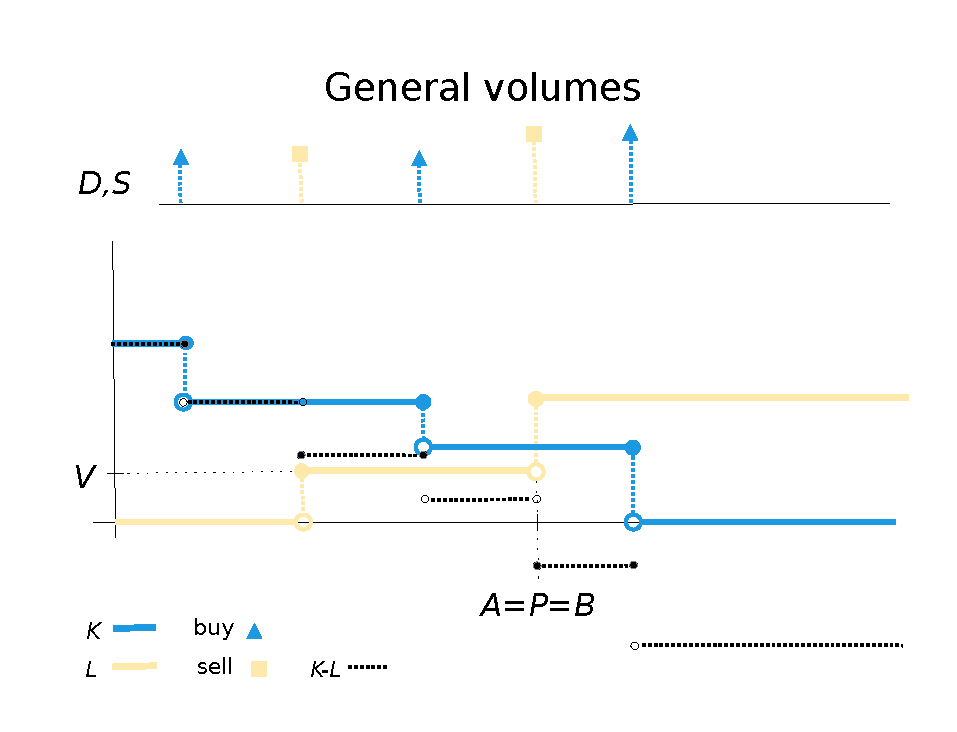
\includegraphics[width=6cm]{nuob.pdf}
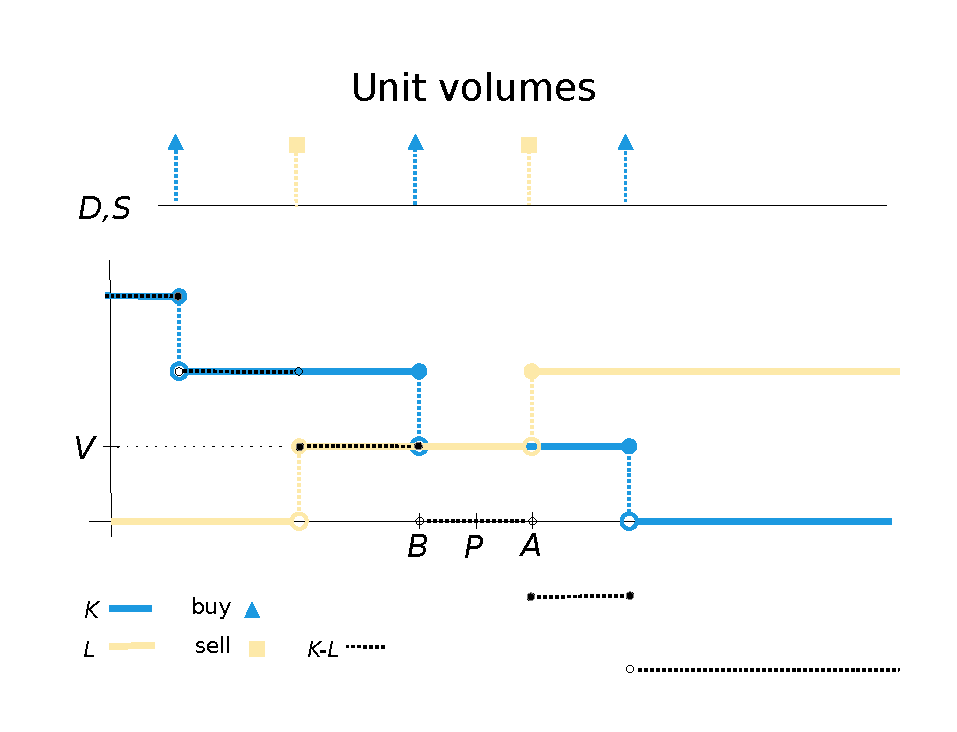
\includegraphics[width=6cm]{ob.pdf}
\end{center}
\caption{Call auction with general order volumes (left) and unit order volumes (right), respectively.}
\label{fig:ob}
\end{figure}

Formally, denoting $K(\pi)=D[\pi,d)$ and $L(\pi)=S(c,\pi]$, $\pi\in I$,
(the demand/supply curves), the maximum traded volume is 
\begin{equation}
V = \max_{p \in I} V^-(p),\qquad V^-(p) \defined K(p) \wedge L(p),
\label{eq:vdef}
\end{equation}
and, further denoting $A=\inf\{\pi\in I:K(\pi)<L(\pi)\}$ and $B=\sup\{\pi\in I:K(\pi)>L(\pi)\}$ 
the price limits,
the clearing price is 
$$P=\begin{cases}\frac{B+A}{2} & A \neq d, B \neq c,
\\\undef & \text{otherwise},
\end{cases}
$$
where $\undef\notin\R$ denotes an undefined price (note, however, that, in some cases with $V=0$, $P$ might be defined). See Figure \ref{fig:ob} for an illustration. 

Our setting covers both the case of continuous limit prices (atoms of $D$ and $S$ may find themselves anywhere in $I$) and the case of discrete prices (atoms of $D$ and $S$ can find themselves only in discrete points, corresponding to price ticks). Note that we do not require the weights (volumes) to be integers. 

Next, we show that $P$ indeed maximizes the traded volume, and, as the traded volume is generally difficult to handle, we introduce its bounds.

\begin{proposition}
(i) 
$$V=\begin{cases} V^-(P) & A \neq d, B \neq c
\\0 & \text{otherwise}
\end{cases}
$$
(ii) For any $p\in I$, $V^-(p) \leq V \leq V^+(p)$ where $V^+(p) = K(p) \vee L(p)$.
\end{proposition}

\begin{proof} (i) When $A = d$ or $B=c$, the assertion is trivial. Let $A \neq d, B \neq c$.
First, note that $V^- = L$ on $(c,A)$ and $V^- = K$ on $(B,d)$. 

Thus, once $B<A$, $V^-$ is non-decreasing on $(c,A)$ and non-increasing on $(B,d)$, which implies that it is constant on $(B,A)$ and  its maximum happens (also on) $(B,A)$, specially in $P$.


If $A=B=P$, then, due to monotonicity, at least one of the following values is equal to $\sup V^-$: $V^-(P-)[=L(P-)],V^-(P+)[=K(P+)]$ or 
$V^-(P)[=K(P) \wedge L(P)=K(P-) \wedge L(P+)]$.
If $K(P-) \geq L(P+)$, then $V^-(P)=L(P+)\geq L(P-)=V^-(P-)$, so only two candidates remain: $V^-(P)[=L(P+)]$ and  $V^-(P+)[=K(P+)]$; however, as the former is strictly greater from the definition of $A$, we proved that the maximum occurs at $P$. Analogously, we can show that $V^-$ is maximized in $P$ if $K(P-) \leq L(P+)$.

\noindent (ii) The first inequality follows directly from (\ref{eq:vdef}). The second one holds trivially if $K(p)=L(p)$ or $V=0$. If $V > 0$ and $K(p)<L(p)$, then $c < B \leq A < p$ hence $P < p$ and, by (i), $V=V^-(P)=K(P) \wedge L(P) \leq L(P) \leq L(p) \leq L(p) \vee K(p)$; similarly for $K(p)>L(p)$.
\end{proof}



\noindent Next we present general formulas for the distribution of random vector $(A,B)$. 

\begin{proposition} \label{th:gen} Let $c<b\leq a \leq d$, put $N_\pi \defined D[\pi,d)-S(c,\pi)$, $\pi \in I$. Then\\
(i) $\P[B<b] = \P[N_b \leq 0]$,\\
(ii)  $\P[A<a] = \P[N_a < 0]$,\\
(iii) $\P[B<b,A<a]=\P[N_b\leq 0]-\P[D[a,d)=S(c,b),S[b,a)=0,D[b,a)=0].$\\
\end{proposition}

\begin{proof} Denote $\Delta = K-L$. As $\Delta$ is a non-decreasing step function, we have
$$[B<b] = [\sup\{\pi\in I:\Delta(\pi)>0\} < b] = [\Delta(b-)\leq 0]$$
and
$$
[A<a] = [\inf\{\pi\in I:\Delta(\pi)< 0 \} < a]
= [\Delta(a-)< 0] 
$$
which proves (i), (ii), respectively because $N_\pi=\Delta(\pi-)$, $\pi \in I$. Further,
\begin{multline*} 
[B<b,A<a] = [\Delta(b-)\leq 0,\Delta(a-)< 0] = [\Delta(b-) < 0] \cup [\Delta(b-) = 0, \Delta(a-)-\Delta(b-) < 0]
\\
=[\Delta(b-) < 0] \cup ( [\Delta(b-) = 0] \setminus E)
\qquad E \defined [\Delta(b-) = 0,\Delta(a-)-\Delta(b-) = 0].
\end{multline*}
As the union is discrete and the difference is proper, we have
$$
\P[B<b,A<a] = \P[\Delta(b-)\leq 0]-\P E = \P[N_b\leq 0]-\P E.
$$
Employing the monotonicity of $\Delta$ and the fact that it jumps at any atom of $D$ or $S$,  we further get
$$
E = [\underbrace{\Delta(b-)}_{=D[b,d)-S(c,b)}=0,S[b,a) = 0, D[b,a)=0], 
$$
which is equivalent to
$$
E=[D[a,d)=S(c,b),S[b,a)=0,D[b,a)=0]
$$
proving (iii).
\end{proof}


\noindent If the offered/ordered volumes are always unit and the atoms of $D$ and $S$ do not coincide w.p.1, then  $K-L$ has unit jumps (down) w.p.1, implying that $B < A$ and, consequently, $V=K(P)=L(P)$ whenever $P\neq \undef$ (note that $V=0$ if $P=\undef$), so we are able to evaluate the joint distribution of $(A,B,V)$:

\begin{proposition} \label{th:general} Let the atoms of $D+S$ have unit weights w.p.1. Then, for any $c< b \leq a < d$ and any $X \subseteq \N_0$,
\begin{equation}
\P[B<b,A>a,V\in X]=\P[ D[b,a] = 0, S[b,a] = 0, D(a,d)=S(c,b)\in X].
\label{eq:pbax}
\end{equation}
\end{proposition}

\begin{proof} Denote $p = \frac{a+b}2$. As $\Delta \defined K-L$ is non-increasing, we have
\begin{multline*}
[B < b,A > a] = [\sup\{\pi\in I:\Delta(\pi)>0\} < b \leq a < \inf\{\pi\in I:\Delta(\pi)< 0 \} ]
\\= [\Delta(b-)\leq 0,\Delta(a+)\geq 0] = [\Delta(b-) = 0,\Delta(a+) = 0]
= [\Delta(b-)=0, \Delta(b-)-\Delta(a+)=0]
\\=[D[b,d)=S(c,b), D[b,a] = 0, S[b,a] = 0]
=[ D(a,d)=S(c,b), D[b,a] = 0, S[b,a] = 0].
\end{multline*}
Therefore and as $B<b,A>a \Rightarrow V=D(a,d)=S(c,b)$, we get (\ref{eq:pbax}).

\end{proof}



\section{Completely Random Order Books}
\label{sec:cr}

Next, we discuss the special case where $D$ and $S$ are mutually independent and completely random. Recall that a random measure $M$ on $(I, \B(I))$ is {\em completely random} if, for any disjoint $S_1,\dots,S_k\in \B(I)$, $MS_1,\dots,MS_k$ are independent. Note also that the class of completely random measures embraces (marked) diffuse Poisson point processes (viewed as measures) as well as the measures with fixed atoms with mutually independent weights (usable in discrete price settings). In fact, any completely random purely atomic measure is a sum of a measure of the former type and a measure of the latter type (see \cite{daley03}, Theorem 10.1.III). 

It is well known (see, e.g. \cite{daley03}, 2.1.6 and 10.1.VI) that a measure $M=\sum_{i=1}^N W_i \delta_{U_i}$, where $\delta_x$ is the Dirac measure concentrated in $x$, $N$ is Poisson, $U_i$'s are i.i.d,, $W_i$'s are i.i.d. and $N,U_1,W_1,U_2,\dots$ are mutually independent (the setting studied by \cite{toke2015exact}) is completely random, but stops to be so once $N$ becomes deterministic (which is the case studied by \cite{derksen2020clearing}); consider $M=\delta_U$ with random $U$, for instance. Further note that, once the process of order arrivals is Poisson and the orders are possibly canceled with a fixed rate, dependent only on the limit price, then the process of valid orders is still Poisson and the corresponding order book is still completely random and Poisson (see, e.g. \cite{smid16estimation}, Example 2.3).


The following result stems directly from Proposition \ref{th:gen}:

\begin{proposition}
\label{cor:cr} If $D \indep S$ and both $D$ and $S$ are completely random, then, for any $c < b \leq a \leq d$,
$$\P[B<b,A<a] = \P[N_b\leq 0]-\P[D[a,d)=S(c,b)]\P[S[b,a)=0]\P[D[b,a)=0]$$
\end{proposition}

\begin{example} Assume discrete prices: $c=0$, $d \in \N$, $D=\sum_{i=1}^{d-1} \delta_i V_i$, 
$S=\sum_{i=1}^{d-1} \delta_i W_i$ where $V_i \sim \mathrm{Bernoulli}(\pi)$, $W_i \sim \mathrm{Bernoulli}(\pi)$, $0 < i < d$, with $V_1,W_1,V_2,\dots,W_{d-1}$ independent. Then
$$
\P[A=d]=\P[B=c]=(1-\pi)^{d-1}, \qquad  \P[A=d, B=c]=(1-\pi)^{2d-2},
$$
and, by Proposition \ref{cor:cr}, for any $0 < a \leq b < d$,
\begin{multline*}
\P[B< b, A < a]
%\\ = \P[D[b,d)-S(c,b)\leq 0]-\P[D[a,d)=S(c,b)] \P[S[b,a)=0]\P[D[b,a)=0]
=
\P[\Bi(d-b,\pi)\stackrel{\indep{}}-\Bi(b-1,\pi)\leq 0] \\ -\P[\Bi(d-a,\pi)\stackrel{\indep{}}-\Bi(b-1,\pi)=0]
\P[\Bi(a-b,\pi)=0]\P[\Bi(a-b,\pi)=0] \\
= \sum_{k=-(b-1)}^0 q_{d-b,b-1,\pi}(k)-q_{d-a,b-1,\pi}(0)(1-\pi)^{2a-2b}
\end{multline*}
where $q_{m,n,\pi}(k) \defined \P[\Bi(m,\pi)\stackrel{\indep{}}-\Bi(n,\pi)=k]$ for any $m,n,\pi,k$. Using this and the fact that $\P[B>A]=0$ we can obtain the distribution of $(A,B)$. In Figure \ref{fig:bin}, this distribution is plotted for $d=11$ and various values of $\pi$.
\end{example}

\begin{figure}
\begin{center}
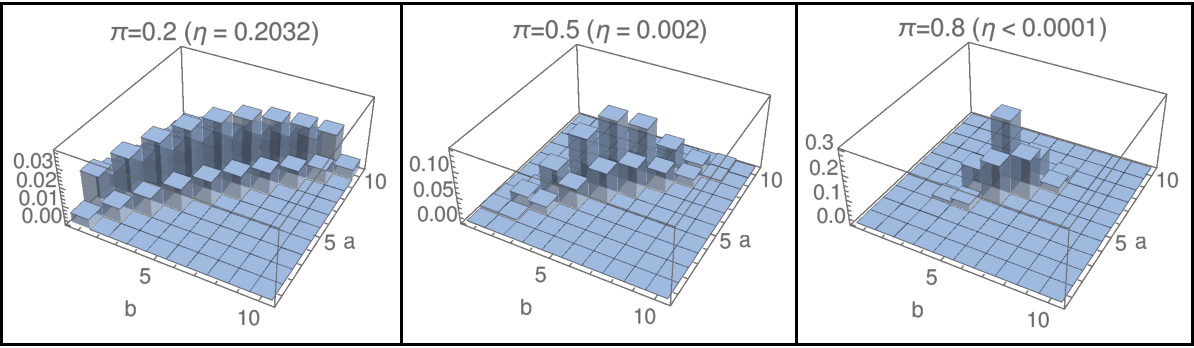
\includegraphics[width=\textwidth]{binom.pdf}
\caption{Distribution of $(A,B)$ in a call auction with $c=0$, $d = 11$, $D=\sum_{i=1}^{d-1} \delta_i V_i$, 
$S=\sum_{i=1}^{d-1} \delta_i W_i$, $V_i \sim \mathrm{Bernoulli}(\pi)$, $W_i \sim \mathrm{Bernoulli}(\pi)$, $0 < i < d$, $\indep(V_1,W_1,V_2,\dots,W_{d-1})$, for various levels of $\pi$. Here, $\eta = \P[B = 0 \vee C = 11]$.}
\label{fig:bin}
\end{center}
\end{figure}


\section{Unit Order Volumes}
\label{sec:cru}

In this subsection, we keep assuming $D\indep S$ to be completely random, but study the special case of the $D$ and $S$ being diffuse (i.e. for any $x\in I$, $D\{x\}=0$, $S\{x\}=0$ w.p.1) and simple (the atoms' weight is always unit). Given these assumptions, by \cite{Kallenberg02}, Theorem 12.10, both $D$ and $S$ are (equivalent to simple) Poisson point processes. Note that, due to our assumption of a finite number of atoms, $D$ and $S$ are fully characterized by 
$\kappa(x)\defined \E K(x)$, $\lambda(x)\defined\E L(x)$, respectively, $x \in I$, with $\kappa(c+)<\infty,\lambda(d-) < \infty$. Let us also recall that we can represent $D=\sum_{i=1}^{N_D} \delta_{V_i}$ where ${N_D}\sim \Po(\kappa(c+))$, the c.d.f. of each $V_i$, $i\in \N$, is $F_D(\bullet)\defined 1-\kappa(\bullet)/\kappa(c+)$, with $\indep (N_D.V_1,V_2,\dots)$ and, similarly, $S=\sum_{i=1}^{N_S} \delta_{W_i}$ where ${N_S}\sim \Po(\lambda(d-))$, the c.d.f. of each $W_i$ is $F_S(\bullet)=\lambda(\bullet)/\lambda(d-)$, and $\indep (N_S.W_1,W_2,\dots)$. 

The following result is a direct consequence of Proposition \ref{th:general}:

\begin{proposition} If $D \indep S$ are (simple) diffuse Poisson, then, for any $c < b \leq a < d$ and $X \subset \N_0$,
\begin{multline}
\P[B<b,A>a,V\in X]=\P[ D[b,a] = 0 ]\P[ S[b,a] = 0]\P[D(a,d)=S(c,b)\in X]\\
= e^{-(\lambda(a)-\lambda(b))}e^{-(\kappa(b)-\kappa(a))}\P[D(a,d)=S(c,b)\in X].
\label{eq:pax}
\end{multline}
\end{proposition}

Applying (\ref{eq:pax}) to single-element $X$'s, we get:
\begin{corollary} For any $c < b \leq a < d$, and $i \in \N_0$,
\begin{multline}
\P[B<b,A>a,V = i] = p(b,a,\{i\}) \\ \defined e^{-(\lambda(a)-\lambda(b))}e^{-(\kappa(b)-\kappa(a))} e^{-\kappa(a)} \frac{\kappa(a)^i}{i!}e^{-\lambda(b)} \frac{\lambda(b)^i}{i!}
 = e^{-\kappa(b)-\lambda(a)} \frac{\kappa(a)^i}{i!}\frac{\lambda(b)^i}{i!}.
\label{eq:pbai}
\end{multline}
\end{corollary}
Further, by taking $X = \N_0$ and using the fact that, for any $\mu\geq 0$ and $\nu \geq 0$, $\P[\Po(\mu)\stackrel{\indep{}}{-}\Po(\nu)=0]=e^{-\mu-\nu}I_{0}(2\sqrt{\mu\nu})$ where $I_0$ is the zero-order modified Bessel function of the first kind (see e.g. \cite{skellam1946frequency}), we get:
\begin{corollary} For any $c < b\leq a < c$,
\begin{equation}
\P[B<b,A>a]=p(b,a,\N_0) \defined e^{-\kappa(b)-\lambda(a)} I_{0}(2\sqrt{\kappa(a)\lambda(b)}).
\label{eq:pba}
\end{equation}
\end{corollary}
\begin{remark}
Equivalently, we can sum (\ref{eq:pbai}) to get,
$$
p(b,a,\N_0)=e^{-\kappa(b)-\lambda(a)}\sum_{i=0}^\infty\frac{(\kappa(a)\lambda(b))^i}{i!i!}.
$$
\end{remark}
As $\P[B\geq A]=0$, (\ref{eq:pbai}) and (\ref{eq:pba}) suffice to evaluate the distributions of $(A,B,V)$, $(A,B)$, respectively.

Assume, until the end of this Section, that $\kappa$ and $\lambda$ are differentiable.

\begin{proposition}
\label{th:abv}
Let either $X = \N_0$ or $X = \{i\}$ for some $i\in \N_0$. Then, for any $Q\in\B([c,d)\times(c,d])$,
\begin{multline}
\P[(B,A,V)\in Q \times X]=\int_{\{(b,a)\in Q: c<b<a<d\}}\gamma(b,a,X)dadb\\
+\charf [0\in X] \left[\int_{\{a:(c,a) \in Q \}}\alpha(a)da
+\int_{\{b:(b,d) \in Q \}}\beta(b)db+\charf[(c,d)\in Q]e^{-\kappa(c)-\lambda(d)}
\right],
\label{eq:pbc}
\end{multline}
where 
$$
\alpha(a)\defined 
\lambda'(a)e^{-\kappa(c)-\lambda(a)},\qquad
\beta(b)\defined-\kappa'(b)e^{-\kappa(b)}{}^{-\lambda(d)},
$$
and
$$
\gamma(b,a,X) = -\frac{\partial}{\partial a\partial b}p(b,a,X).
$$
\end{proposition}

\begin{proof}
See Appendix \ref{app:abv}.
\end{proof}

\begin{corollary}\label{cor:abdens} For any $Q\in\B([c,d)\times(c,d])$,
\begin{multline*}
\P[(B,A)\in Q]=\int_{\{(b,a)\in Q, b \in I, a \in I\}}g(b,a)dadb\\
+\int_{\{a:(c,a) \in Q \}}\alpha(a)da
+\int_{\{b:(b,d) \in Q \}}\beta(b)db+\charf[(c,d)\in Q]e^{-\kappa(c)-\lambda(d)}
\end{multline*}
where 
$$g(b,a)=0,\qquad a<b, $$
and
\begin{multline}
g(b,a)
%= e^{-\kappa(b)-\lambda(a)}
%\left(
%-\kappa'(b)\lambda'(a) \sum_{i=0}^\infty \frac{\lambda(b)^i\kappa(a)^i}{i!i!}
%+\kappa'(a)\kappa'(b) \sum_{i=0}^\infty \frac{\lambda(b)^{i+1}\kappa(a)^i}{(i+1)!i!}
%\right.
%\\
%\left.
%+\lambda'(b)\lambda'(a) \sum_{i=0}^\infty \frac{\lambda(b)^{i}\kappa(a)^{i+1}}{(i+1)!i!}
%-\lambda'(b)\kappa'(a) \sum_{i=0}^\infty \frac{\lambda(b)^{i}\kappa(a)^{i}}{i!i!}
%\right)\\
= e^{-\kappa(b)-\lambda(a)}
\left(
-\left[\kappa'(b)\lambda'(a)+\lambda'(b)\kappa'(a)\right] I_0(2\sqrt{\kappa(a)\lambda(b)})
\right.
\\
\left.
+\left[\kappa'(a)\kappa'(b)
\sqrt{\frac{\lambda(b)}{\kappa(a)}}
+\lambda'(a)\lambda'(b)
\sqrt{\frac{\kappa(a)}{\lambda(b)}}\right] I_1(2\sqrt{\kappa(a)\lambda(b)})
\right), \qquad a \geq b,
\label{eq:gamma}
\end{multline}
where $I_k$ is the modified Bessel function of $k$ -th order of the first kind; we take $\kappa'(a)\sqrt{\frac{\lambda(b)}{\kappa(a)}}=0$ whenever $\kappa(a)=0$ and 
$\lambda'(b)
\sqrt{\frac{\kappa(a)}{\lambda(b)}}=0$ whenever $\lambda(b)=0$.
\end{corollary}



\begin{proof} See Appendix \ref{app:abdens}.
\end{proof}

Furthermore, we evaluate the distribution of $(P,V)$:

\begin{proposition}
Let $X \subseteq \N_0$ be as in Proposition \ref{th:abv}. Then, 
\begin{equation}
\P[P=\undef, V\in X]=\charf[0\in X] [e^{-\kappa(c)}+e^{-\lambda(d)}-e^{-\kappa(c)-\lambda(d)}]\label{eq:pd0}
\end{equation}
and, for any $p\in I$,
\begin{multline}
\P[P<p,P\neq\undef,V\in X]\\=
%\Phi_{\kappa,\lambda}(p)\defined
\int_{c}^{p}\eta(a,a,X)da+\int_{p}^{(2p-c) \wedge d}\eta(2p-a,a,X)da+\charf[0 \in X] [e^{-\kappa(c)-\lambda((2p-c) \wedge d)}-e^{-\kappa(c)}]
\label{eq:pdist}
\end{multline}
where $\eta(b,a,X)=-\frac{\partial}{\partial a} p(b,a,X)$, $b<a$. 
\end{proposition}

\begin{proof}
By Proposition \ref{th:abv}, 
\begin{multline*}
\P[P<p,P\neq\undef,V\in X] =\P[A<d,c<B<2p-A,V\in X]
\\ =\int_{\{a < d\}}\int_{\{ c < b < 2p-a\}}\P_{(B,A,V)}(db,da,X)\\
=\int_{\{c< a < d\}}\int_{\underbrace{\{ c < b < 2p-a, b < a \}}_{\text{$=\emptyset$ for $a \geq 2p-c$}}}\gamma(b,a,X)dbda\\
=\int_c^{(2p-c) \wedge d}\int_c^{a \wedge (2p-a)} \gamma(b,a,X)dbda \\
=\int_c^{(2p-c) \wedge d}[ \eta(a \wedge 2p-a,a,X)da - \eta(c,a,X)]da\\
=\underbrace{\int_c^{(2p-c) \wedge d} \eta(a \wedge 2p-a,a,X)da}_
{=\int_c^p \eta(a, {\dots} + \int_p^{(2p-c) \wedge d} \eta(2p-a,\dots} +
\underbrace{\left[p(c,(2p-c) \wedge d,X)-p(c,c,X)\right]}_{=\charf[0\in X](e^{-\kappa(c)-\lambda((2p-c) \wedge d)}-e^{-\kappa(c)})}
\end{multline*}
(see Appendix \ref{app:abv} for the definition of $p(c,\bullet,X)$).
\end{proof}

\begin{theorem}
(i)
$$
\P[P=\undef]=e^{-\kappa(c)}+e^{-\lambda(d)}-e^{-\kappa(c)-\lambda(d)}.
$$

\noindent (ii) For any $p\in I$ and $v \in \N_0$,
\begin{multline}
\P[P<p,P\neq\undef,V = v]=
%\Phi_{\kappa,\lambda}(p)\defined
\int_{c}^{p}\psi(a,a,v)da \\ +\int_{p}^{(2p-c) \wedge d}\psi(2p-a,a,v)da+\charf[v=0] (e^{-\kappa(c)-\lambda((2p-c) \wedge d)}-e^{-\kappa(c)}),
\label{eq:pdist2}
\end{multline}
where
$$
\psi(b,a,v)=
\begin{cases}
e^{-\kappa(b)-\lambda(a)}\lambda'(a) & v=0,\\
e^{-\kappa(b)-\lambda(a)}\frac{\lambda(b)^v}{v!}\left(\lambda'(a)\frac{\kappa(a)^v}{v!}
- \kappa'(a)\frac{\kappa(a)^{v-1}}{{(v-1)}!}\right) & v>0.
\end{cases}
$$
\noindent (iii) For any $p \in I$,
\begin{multline}
\P[P<p,P\neq\undef]\\=
%\Phi_{\kappa,\lambda}(p)\defined
\int_{c}^{p}\phi(a,a)da+\int_{p}^{2p \wedge d}\phi(2p-a,a)da + [e^{-\kappa(c)-\lambda(2p \wedge d)}-e^{\kappa(c)}],
\label{eq:ppu}
\end{multline}
where 
$$
\phi(b,a)=
e^{-\kappa(b)-\lambda(a)}\left(-\lambda'(a)I_0(2\sqrt{\kappa(a)\lambda(b)})+\kappa'(a)\sqrt{\frac{\lambda(b)}{\kappa(a)}}I_1(2\sqrt{\kappa(a)\lambda(b)})\right)
$$
taking $\kappa'(a)\sqrt{\frac{\lambda(b)}{\kappa(a)}}=0$ whenever $\kappa(a)=0$.

\noindent (iv) For any $v\in \N_0$,
$$
\P[V=v]\\=
%\Phi_{\kappa,\lambda}(p)\defined
\int_{c}^{d}\psi(a,a,v)da + \charf[v = 0] e^{-\lambda(d)}.
$$
\end{theorem}

\begin{proof} (i) follows from (\ref{eq:pd0}), (ii) and (iii) follow from (\ref{eq:pdist}), to get (iv), it suffices to take the limit $p\rightarrow d$ in (\ref{eq:pdist}).
\end{proof}

\begin{corollary} \label{cor:dens}
 $P$ is absolutely continuous w.r.t. $\delta_\undef+\ell((c,d))$, where $\ell$ denotes the Lebesgue measure, with density 
\begin{equation}
f(\undef)=e^{-\kappa(c)}+e^{-\lambda(d)}-e^{-\kappa(c)-\lambda(d)},\qquad 
f(p)=2 \int_p^{2 p \wedge d} g(2p-a,a) da.
\label{eq:pdens}
\end{equation}
\end{corollary}

\begin{proof} See Appendix \ref{app:dens}.
\end{proof}




 

\section{Random Order Volumes}
\label{sec:crr}

In the present Section, we release the assumption of unit weights, still assuming that $D\indep S$ are diffuse complete random, but allowing for (i.i.d.) random weights with the same distribution for buy-- and the sell orders. Under these assumptions, the locations of the $D$'s and $S$'s atoms form a (diffuse) Poisson point processes, which we denote $D_g$, $S_g$, respectively.

\def\cpo{\mathrm{CPo}}

\begin{theorem} Let $D \indep S$, let $D_g$, $S_g$ be diffuse Poisson and let the weights of the atoms be i.i.d., following a distribution $\L$ such that $\L(-\infty,0]=0$. Then, for any $c < b \leq a < d$,
\begin{equation}
\label{eq:pbcp}
\P[B<b] = \P[\mathcal{C}(\kappa_g(b),\lambda_g(b),\L)\leq 0],
\end{equation}
\begin{equation}
\label{eq:pacp}
\P[A<a] = \P[\mathcal{C}(\kappa_g(a),\lambda_g(a),\L)< 0],
\end{equation}
and
\begin{multline*}
\P[B<b,A<a] = \P[\mathcal{C}(\kappa_g(b),\lambda_g(b),\L)\leq 0]
\\
- e^{-(\lambda_g(a)-\lambda_g(b))}e^{-(\kappa_g(b)-\kappa_g(a))}\P[\mathcal{C}(\kappa_g(a),\lambda_g(b),\L)=0];
\end{multline*}
here, $\kappa_g(\pi)=\E D_g[\pi,d)$, $\lambda_g(\pi)=\E S_g(c,\pi]$, $\pi \in I$, and $\mathcal{C}(\kappa,\lambda,\L)$ is the Compound Poisson distribution with intensity $\kappa+\lambda$ and embedded distribution $\frac\kappa{\kappa+\lambda} \L + \frac\lambda{\kappa+\lambda} \L^-$ where $\L^-$ is  the $\L$'s negative version (i.e. $\L(x,\infty)=\L^-(-\infty,-x)$, $x \in \R$).
\end{theorem}
\begin{proof}
The assertion follows from Proposition \ref{cor:cr}, using the fact that the convolution of two compound Poisson distributions is compound Poison with properly weighted mixed embedded distribution.
\end{proof}

%https://www.sciencedirect.com/science/article/abs/pii/0167637784900087

\noindent In the following Theorem, we evaluate the asymptotic distributions of the clearing price and the bounds of the traded volume.

\begin{theorem} \label{th:asymp} Let $\kappa_0,\lambda_0:I\rightarrow \R_+$ be strictly increasing, decreasing, respectively, and differentiable. Let $\L$ be distribution with $\L(-\infty,0]=0$ having a finite third moment. For any $n \in \N$, let $P_n,B_n,A_n,\dots$ be the clearing price, lower price limit, upper price limit, etc., in a call auction with independent compound Poisson order books defined by $\kappa_g = n \kappa_0$ and $\lambda_g = n\lambda_0$ and the atoms' weight distribution $\L$. Let $p$ be the solution of the equation $\kappa_0(p)= \lambda_0(p)$. Then\\
(i) $$P_n\stackrel{P}\longrightarrow p$$
(ii)
\begin{multline*}
\sqrt{n}(P_n-p) \stackrel{d} \longrightarrow \ND\left(0,v_gr_\L\right), 
\\ 
v_g \defined \frac{\kappa_0(p)+\lambda_0(p)}{(\lambda_0'(p)-\kappa_0'(p))^2}=\frac{2\kappa_0(p)}{(\lambda_0'(p)-\kappa_0'(p))^2}
=
\frac{2\lambda_0(p)}{(\lambda_0'(p)-\kappa_0'(p))^2},
\qquad
r_\L = \frac{\E \L^2}{(\E \L)^2},
\end{multline*}
where  $\E\L$ and $\E\L^2$ are the $\L$'s expectation, (non-central) second moment, respectively.\\
(iii) 
$$W^-_n \leq V_n \leq W^+_n,\qquad 
W^-_n \defined V_n^-(p),\qquad W_n^+ \defined V_n^+(p),$$
with
$$
\frac{1}{\sqrt{n}}(W_n^--n \mu)\stackrel{d}\longrightarrow \mathcal{M}_{w}, 
\qquad 
\frac{1}{\sqrt{n}}(W_n^+-n \mu)\stackrel{d}\longrightarrow \mathcal{M}^{w};
$$
$$
\mu = \kappa_0(p) \E\L = \lambda_0(p) \E\L, \quad
w = 
\kappa_0(p) \E \L^2= \lambda_0(p) \E \L^2,
$$
where $\mathcal{M}_w$, $\mathcal{M}^w$, are the distributions of the minimum, maximum, respectively, of two independent $\ND(0,w)$ random variables. In particular
$$
\P\left[ \frac{1}{\sqrt{n}}(W^-_n-n \mu)  < x
\right] = 1-\left(1-\varphi\left(\frac{x}{\sqrt{w}}\right) \right)^2,
$$
$$
\P\left[ \frac{1}{\sqrt{n}}(W^+_n-n \mu) < x
\right] = \varphi\left(\frac{x}{\sqrt{w}}\right)^2,
$$
where $\varphi$ is the standard normal c.d.f.
\end{theorem}

\begin{proof} See Appendix \ref{app:asymp}.
\end{proof}


\begin{corollary}
If, in Theorem \ref{th:asymp}, $\L = \delta_1$ (i.e., the volumes are deterministic and unit), then the Theorem holds with 
$v_g = \frac{2\kappa(p)}{[\lambda'(p)-\kappa'(p)]^2}$, $r_L=1$, $\mu = w = \kappa(p)=\lambda(p)$.
\end{corollary}

\paragraph*{Numerical Illustration.}
Once the trading intensities are high enough, we can represent $P=P_n$, $V^-(p)=V_n^-(p)$ and $V^+(p)=V_n^+(p)$ for some $n$ and approximate
$$
P \quad \dot \sim \quad 
\ND\left(p,\frac{2\kappa_g(p)\E\L^2}{(\kappa'_g(p)-\lambda'_g(p))^2(\E \L)^2} \right ),
$$
and
$$
W^- \leq V \leq W^+,
$$
where
$$
\P\left[ W^-  < x
\right] \doteq 1-\left(1-\varphi\left(\frac{\kappa_g(p)\E \L+x}{\sqrt{\kappa_g(p)\E \L^2}}\right) \right)^2
$$
$$
\P\left[ W^+ < x
\right] \doteq \varphi\left(\frac{\kappa_g(p)\E \L+x}{\sqrt{\kappa_g(p)\E \L^2}}\right)^2
$$
$x \in I$. In Figure \ref{fig:il}, we illustrate the accuracy of these approximations for various levels of trading intensity: we assume that order volumes and intensities are multiples of linear functions, different for demand and supply. It can be seen that the approximations are nearly perfect, once there are tens of orders on both sides (recall that the expected number of buy and sell orders equals $\kappa(c+)$, $\lambda(d-)$, respectively.

\begin{remark} As, by the Schwarz inequality, $r_\L \geq 1$, with the minimum achieved by $\L = \delta_1$, we see that taking randomness of the order volumes into account leads to higher (asymptotic) variance of both the price and the volume bounds in comparison with the usual approximation of the volumes by their mean values (normed to one). 
\end{remark}

Next, we compare our asymptotic result with that of \cite{derksen2020clearing}:

\begin{remark} Consider
$$
D=\sum_{i=1}^{N_D} \delta_{D_i}, \qquad S=\sum_{i=1}^{N_S} \delta_{S_i}
$$
where $\E N_D=(1-\alpha)n$, $\E N_S=\alpha n$ for some $\alpha \in (0,1)$ and $n\in \N$,  $D_i$, $i\in\N$, being i.i.d. with strictly increasing absolutely continuous c.d.f. $F_D$, and $S_i$, $i\in \N$ being i.i.d. with strictly increasing a.c. c.d.f $F_S$, such that all the variables are mutually independent.

Once $N_S$ and $N_D$ are Poisson, $D$ and $S$ are Poisson processes determined by 
$$
\kappa(x)=n (1-\alpha) (1-F_D(x)), \qquad \lambda(x)=n \alpha F_S(x),
$$
and, by Theorem \ref{th:asymp},
$$
\sqrt{n}(P_n-p) \rightarrow_n \ND(0,v), 
\qquad 
v=\frac{ 2 \alpha F_S(p) }{[(1-\alpha)f_D(p)+\alpha f_S(p)]^2}.
$$
 

If, instead, $N_D=(1-\alpha) n$ and $N_S = \alpha n$ are deterministic, we have, by Theorem 3.1 of \cite{derksen2020clearing}, that 
$$
\sqrt{n}(P_n-p) \rightarrow_n \ND(0,\tilde v), 
\qquad 
\tilde v=\frac{ \alpha [F_D(p)+ (1-F_S(p))]F_S(p)}{[(1-\alpha)f_D(p)+\alpha f_S(p)]^2}
$$
By comparison of the asymptotic variances we see that assuming random order numbers increases the price variance significantly compared with only using their expectations. 
\end{remark}


\begin{figure}
\begin{center}
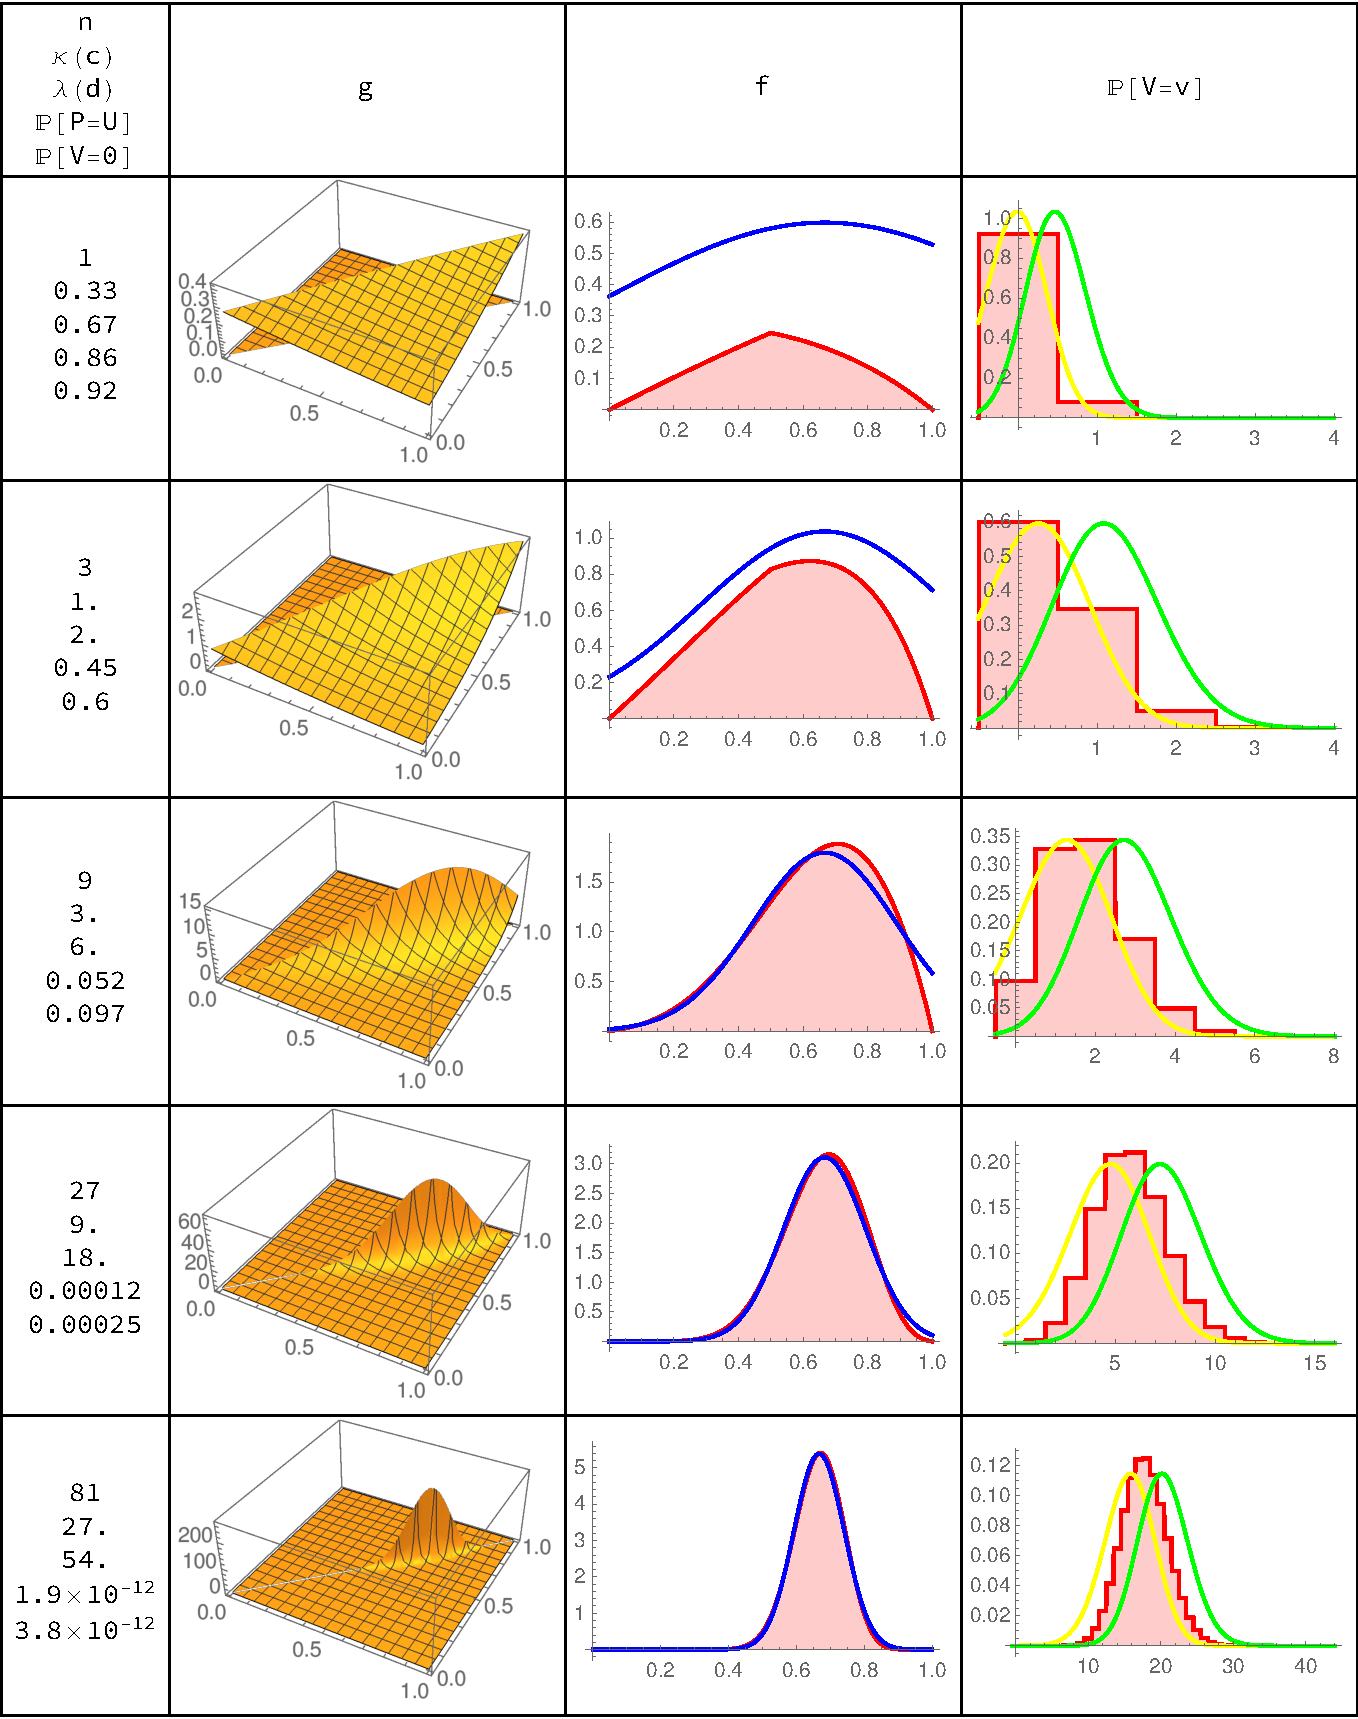
\includegraphics[width=\textwidth]{illust.pdf}
\caption{Distribution of $(A,B)$, $P$ and $V$ for $\kappa(a)=n \frac{2}{3}(1-a)$, $\lambda(b)=n \frac{1}3 b$ and unit order volumes. Blue, normal approximation of $P$, yellow, normal approximation of $W^-$, green, normal approximation of $W^+$. }
\label{fig:il}
\end{center}
\end{figure}

\section{Conclusions}

We have thoroughly studied a natural stochastic model of call auction. We have described both the exact and the asymptotic distributions in various special cases of this model. The next natural step could be to describe the dynamics of repeated call auctions, suggested by \cite{budish2015high}, and compare it with that of the continuous double auction.

\paragraph*{Acknowledgments} This work was supported by grant No. GA19-11062S from the Czech Science Foundation. Computational resources were partially provided by the ``eInfrastruktura CZ'' (e-INFRA CZ LM2018140) project supported by the Ministry of Education, Youth and
Sports of the Czech Republic

%\bibliographystyle{APT}
\footnotesize
%\bibliography{../../smid}
\documentclass{aptpub}
\usepackage{graphicx}
\usepackage{hyperref}
\authornames{\v Sm\'\i d, Kub\v ena} % insert the authors here for use in running head. If three or more authors please use (for example) M.~YARROW {\it et al}. Author names should follow the same M.~YARROW format and if two authors, separate by 'AND'.
\shorttitle{Distribution of Call Auction} % insert short title here for use in running head

% Put any of your own definitions here.

%\numberwithin{equation}{section}  % If you number theorems, etc. within sections,
                                   % then please uncomment this line to number
                                   % equations with sections too.

\global\long\def\P{\mathbb{P}}%
\global\long\def\N{\mathbb{N}}%
\global\long\def\U{\mathbb{U}}%
\global\long\def\E{\mathbb{E}}%
\global\long\def\R{\mathbb{R}}%
\global\long\def\G{\mathcal{G}}%
\global\long\def\g{\mathbb{\Pi}}%
\global\long\def\F{\mathcal{F}}%
\global\long\def\S{\mathbb{S}}%
\global\long\def\Q{\mathcal{Q}}%
\global\long\def\B{\mathcal{B}}%
\global\long\def\ND{\mathcal{N}}%
\global\long\def\XX{\mathcal{X}}%
\global\long\def\indep#1{{\perp\hspace{-2mm}\perp}#1}%
\global\long\def\L{\mathcal{L}}%
\global\long\def\var{\mathrm{var}}%
\global\long\def\cov{\mathrm{cov}}%
\global\long\def\charf{\mathbf{1}}%
\global\long\def\d{\mathrm{d}}%
\global\long\def\M{\mathcal{M}}%
\global\long\def\Exp{\mathrm{Exp}}%
\global\long\def\Uniform{\mathrm{U}}%
\global\long\def\eqd{\stackrel{d}{=}}%
\global\long\def\eqas{\stackrel{a.s.}{=}}%
\global\long\def\X{\mathcal{X}}%
\global\long\def\supp{\mathrm{support}}%
\global\long\def\H{\mathcal{H}}%
\global\long\def\Z{\mathcal{Z}}%
\global\long\def\as{\qquad a.s.}%
\global\long\def\on{\qquad\text{on }}%
\global\long\def\C{\mathcal{C}}%
\global\long\def\barxi{\overline{\xi}}%
\global\long\def\Po{\mathrm{Po}}%
\global\long\def\Bi{\mathrm{Bi}}%
\global\long\def\Be{\mathrm{Be}}%
\global\long\def\defined{\stackrel{\text{def}}{=}}%
\global\long\def\barA{\overline{A}}%
\global\long\def\A{\mathcal{A}}%
\global\long\def\barx{x}%
\global\long\def\barX{TBD}%
\global\long\def\last{\ell}%
\global\long\def\bary{y}%
\global\long\def\barz{z}%
\global\long\def\DD{\mathcal{D}}%
\global\long\def\undef{\mathfrak{U}}


\begin{document}%\recd{}{}%Do not alter this line.

\title{Distribution of Price and Volume in Call Auction} % insert title - use `\\ if it requires more than one line.

\authorone[Czech Academy of Sciences]{Martin   \v Sm\'\i d} 
%Affiliation is just the name of your university or institution, for example 'University of Sheffield'. Author names should be of the form 'Mark Yarrow'. 
%Authors should be ordered alphabetically subject to the convention in that particular authors country. For example 'Remco van der Hofstad' would be listed under 'H' as is standard in the Netherlands. 
\authortwo[Czech Academy of Sciences]{Ale\v s Anton\`\i n Kub\v ena} 

%Please use the following format for addresses and emails. The APT office will sort this out after you submit your files.
\addressone{Institute of Information Theory and Automation of the CAS. Pod Vod\' arenskou v\v e\v z\'\i 4, Praha 8, 182 00, Czech Republic,
              Tel.: +420-2-66052400} % Your postal address goes here.
\emailone{smid@utia.cas.cz} %Authors email goes here.

\begin{abstract}

We describe exact and asymptotic distributions of the settlement price and the traded volume in call auction. On top of existing results, we allow completely random order books and random order volumes. We show that approximating random order volumes and/or order numbers by constants leads to a significant underestimation of both the settlement price and the traded volume variances. We also demonstrate a rapid speed of convergence of the asymptotic distributions to the exact ones. 
%, which is a trading mechanism accumulating demand and supply for some time period and then settling them for a price maximizing the traded volume. 

\end{abstract}

\keywords{call auction, settlement price, traded volume, exact distribution, asymptotic distribution}%insert keywords separated by a semicolon. You should avoid including keywords which also appear in the title.

\ams{91G15}{60G57}% insert the primary 2020 Maths Subject Classification number in the first bracket
		% and the secondary ams number(s) in the second bracket
		% e.g. \ams{60E20}{49G03;49F10}
		%Maximum of three in each, ideally one or two in each primary and secondary.
		%codes found here ``https://mathscinet.ams.org/msnhtml/msc2020.pdf''


\section{Introduction}

Yet trading on today's financial markets is mostly continuous \cite{friedman2018double}, the days of {\em call auction} -- a simpler trading mechanism in which the price is being determined at fixed time instants rather than after each order arrival -- are far from being numbered. Call auctions are used to determine closing and opening prices in electronic markets \cite{toke2015exact}, and there are even suggestions to replace continuous trading by frequent batch auctions to avoid time arbitrage \cite{budish2015high}. 

In comparison with its continuous counterpart, relatively little scientific attention has been paid to call auction. Seminal work \cite{mendelson1982market} studies its simple model with unit order volumes and uniform limit price distributions. Paper \cite{toke2015exact}  generalizes these results, analytically describing the exact and asymptotic marginal distributions of traded volume and the price limits given a general (absolutely continuous) limit price distribution, which is the same for buy and sell orders, but an imbalance of arrival rates is allowed. More recent work \cite{derksen2020clearing} allows for differently distributed buy-- and sell limit prices; moreover, a (deterministic) excess liquidity may exist. An analytical formula is derived for the exact {\em conditional joint} distribution of the clearing price and the traded volume given the order numbers, as well as an asymptotic formula for the {\em unconditional} distribution of the clearing price given that the {\em deterministic} numbers of orders grow to infinity. 

We present more general results as we assume random order volumes and
derive general formulas for the {\em exact unconditional} joint distributions of price limits and, given unit order sizes, also for the {\em exact unconditional} joint distribution of the price limits and the traded volume (Section \ref{sec:call}). 

Further, we derive more detailed formulas for the case in which the order books (i.e. the collections of orders of the same type) are completely random (i.e. Poisson or having discrete limit prices with independent volumes, Section \ref{sec:cr}). In the special case of unit order sizes, we describe the exact joint distribution of the price and the traded volume (Section \ref{sec:cru}) and, for the general case, we derive asymptotic (marginal) distributions of the price and the bounds for the traded volume (Section \ref{sec:crr}). Finally, we numerically illustrate that the convergence of the asymptotic distributions to their exact counterparts is rapid.

It turns out that both the randomness of the order numbers and the randomness of the traded volumes matter, significantly increasing the price (asymptotic) variance compared to the approximations assuming unit orders \cite{mendelson1982market,toke2015exact,derksen2020clearing} and/or deterministic order numbers \cite{derksen2020clearing}.




\section{Call Auction}
\label{sec:call}

We first describe the call auction. Let $I=(c,d)$, $c\in\R_{-\infty}$, $d\in\R_{\infty}$ be an open
interval of possible prices and let $D,S$ be atomic random measures with finitely many atoms,
describing the order books. In particular, each atom of $D$/$S$ represents a buy/sell
limit order with the limit price corresponding to the atom's location and the ordered/offered volume corresponding to its weight.
Let us recall that a buy/sell limit order is a commitment to buy/sell a specified {\em volume} for no more/no less than a specified {\em limit price}.

There are more ways to choose the clearing price. Usually, one of the prices is chosen that maximizes the volume traded. In this work, we take the average value for which the demand and supply curves actually intersect as the clearing price.

\begin{figure}
\begin{center}
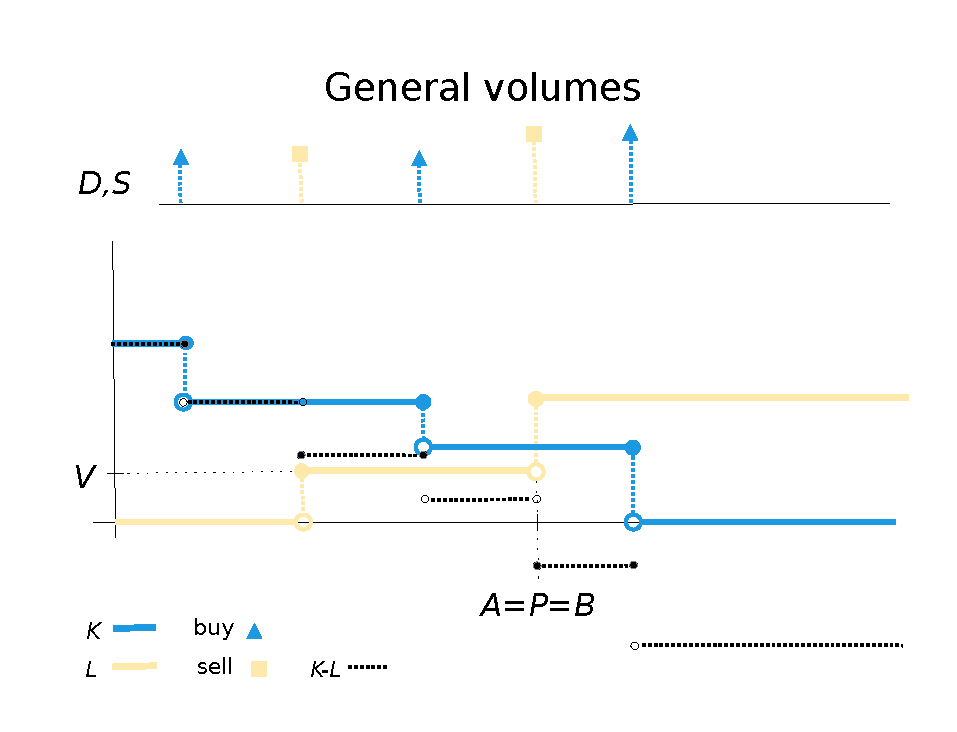
\includegraphics[width=6cm]{nuob.pdf}
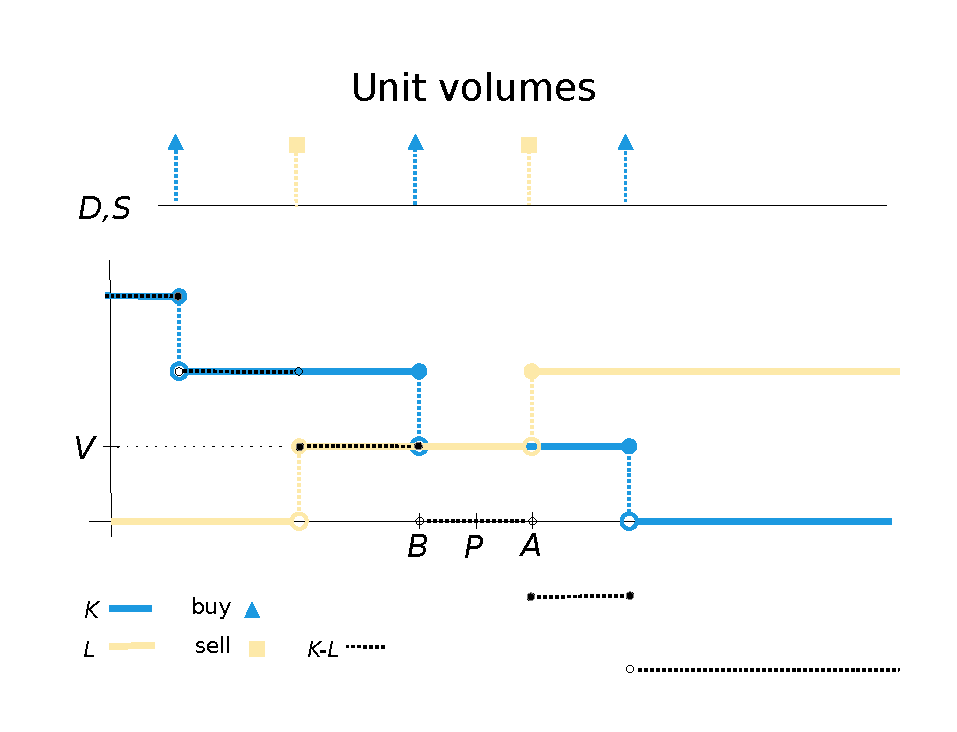
\includegraphics[width=6cm]{ob.pdf}
\end{center}
\caption{Call auction with general order volumes (left) and unit order volumes (right), respectively.}
\label{fig:ob}
\end{figure}

Formally, denoting $K(\pi)=D[\pi,d)$ and $L(\pi)=S(c,\pi]$, $\pi\in I$,
(the demand/supply curves), the maximum traded volume is 
\begin{equation}
V = \max_{p \in I} V^-(p),\qquad V^-(p) \defined K(p) \wedge L(p),
\label{eq:vdef}
\end{equation}
and, further denoting $A=\inf\{\pi\in I:K(\pi)<L(\pi)\}$ and $B=\sup\{\pi\in I:K(\pi)>L(\pi)\}$ 
the price limits,
the clearing price is 
$$P=\begin{cases}\frac{B+A}{2} & A \neq d, B \neq c,
\\\undef & \text{otherwise},
\end{cases}
$$
where $\undef\notin\R$ denotes an undefined price (note, however, that, in some cases with $V=0$, $P$ might be defined). See Figure \ref{fig:ob} for an illustration. 

Our setting covers both the case of continuous limit prices (atoms of $D$ and $S$ may find themselves anywhere in $I$) and the case of discrete prices (atoms of $D$ and $S$ can find themselves only in discrete points, corresponding to price ticks). Note that we do not require the weights (volumes) to be integers. 

Next, we show that $P$ indeed maximizes the traded volume, and, as the traded volume is generally difficult to handle, we introduce its bounds.

\begin{proposition}
(i) 
$$V=\begin{cases} V^-(P) & A \neq d, B \neq c
\\0 & \text{otherwise}
\end{cases}
$$
(ii) For any $p\in I$, $V^-(p) \leq V \leq V^+(p)$ where $V^+(p) = K(p) \vee L(p)$.
\end{proposition}

\begin{proof} (i) When $A = d$ or $B=c$, the assertion is trivial. Let $A \neq d, B \neq c$.
First, note that $V^- = L$ on $(c,A)$ and $V^- = K$ on $(B,d)$. 

Thus, once $B<A$, $V^-$ is non-decreasing on $(c,A)$ and non-increasing on $(B,d)$, which implies that it is constant on $(B,A)$ and  its maximum happens (also on) $(B,A)$, specially in $P$.


If $A=B=P$, then, due to monotonicity, at least one of the following values is equal to $\sup V^-$: $V^-(P-)[=L(P-)],V^-(P+)[=K(P+)]$ or 
$V^-(P)[=K(P) \wedge L(P)=K(P-) \wedge L(P+)]$.
If $K(P-) \geq L(P+)$, then $V^-(P)=L(P+)\geq L(P-)=V^-(P-)$, so only two candidates remain: $V^-(P)[=L(P+)]$ and  $V^-(P+)[=K(P+)]$; however, as the former is strictly greater from the definition of $A$, we proved that the maximum occurs at $P$. Analogously, we can show that $V^-$ is maximized in $P$ if $K(P-) \leq L(P+)$.

\noindent (ii) The first inequality follows directly from (\ref{eq:vdef}). The second one holds trivially if $K(p)=L(p)$ or $V=0$. If $V > 0$ and $K(p)<L(p)$, then $c < B \leq A < p$ hence $P < p$ and, by (i), $V=V^-(P)=K(P) \wedge L(P) \leq L(P) \leq L(p) \leq L(p) \vee K(p)$; similarly for $K(p)>L(p)$.
\end{proof}



\noindent Next we present general formulas for the distribution of random vector $(A,B)$. 

\begin{proposition} \label{th:gen} Let $c<b\leq a \leq d$, put $N_\pi \defined D[\pi,d)-S(c,\pi)$, $\pi \in I$. Then\\
(i) $\P[B<b] = \P[N_b \leq 0]$,\\
(ii)  $\P[A<a] = \P[N_a < 0]$,\\
(iii) $\P[B<b,A<a]=\P[N_b\leq 0]-\P[D[a,d)=S(c,b),S[b,a)=0,D[b,a)=0].$\\
\end{proposition}

\begin{proof} Denote $\Delta = K-L$. As $\Delta$ is a non-decreasing step function, we have
$$[B<b] = [\sup\{\pi\in I:\Delta(\pi)>0\} < b] = [\Delta(b-)\leq 0]$$
and
$$
[A<a] = [\inf\{\pi\in I:\Delta(\pi)< 0 \} < a]
= [\Delta(a-)< 0] 
$$
which proves (i), (ii), respectively because $N_\pi=\Delta(\pi-)$, $\pi \in I$. Further,
\begin{multline*} 
[B<b,A<a] = [\Delta(b-)\leq 0,\Delta(a-)< 0] = [\Delta(b-) < 0] \cup [\Delta(b-) = 0, \Delta(a-)-\Delta(b-) < 0]
\\
=[\Delta(b-) < 0] \cup ( [\Delta(b-) = 0] \setminus E)
\qquad E \defined [\Delta(b-) = 0,\Delta(a-)-\Delta(b-) = 0].
\end{multline*}
As the union is discrete and the difference is proper, we have
$$
\P[B<b,A<a] = \P[\Delta(b-)\leq 0]-\P E = \P[N_b\leq 0]-\P E.
$$
Employing the monotonicity of $\Delta$ and the fact that it jumps at any atom of $D$ or $S$,  we further get
$$
E = [\underbrace{\Delta(b-)}_{=D[b,d)-S(c,b)}=0,S[b,a) = 0, D[b,a)=0], 
$$
which is equivalent to
$$
E=[D[a,d)=S(c,b),S[b,a)=0,D[b,a)=0]
$$
proving (iii).
\end{proof}


\noindent If the offered/ordered volumes are always unit and the atoms of $D$ and $S$ do not coincide w.p.1, then  $K-L$ has unit jumps (down) w.p.1, implying that $B < A$ and, consequently, $V=K(P)=L(P)$ whenever $P\neq \undef$ (note that $V=0$ if $P=\undef$), so we are able to evaluate the joint distribution of $(A,B,V)$:

\begin{proposition} \label{th:general} Let the atoms of $D+S$ have unit weights w.p.1. Then, for any $c< b \leq a < d$ and any $X \subseteq \N_0$,
\begin{equation}
\P[B<b,A>a,V\in X]=\P[ D[b,a] = 0, S[b,a] = 0, D(a,d)=S(c,b)\in X].
\label{eq:pbax}
\end{equation}
\end{proposition}

\begin{proof} Denote $p = \frac{a+b}2$. As $\Delta \defined K-L$ is non-increasing, we have
\begin{multline*}
[B < b,A > a] = [\sup\{\pi\in I:\Delta(\pi)>0\} < b \leq a < \inf\{\pi\in I:\Delta(\pi)< 0 \} ]
\\= [\Delta(b-)\leq 0,\Delta(a+)\geq 0] = [\Delta(b-) = 0,\Delta(a+) = 0]
= [\Delta(b-)=0, \Delta(b-)-\Delta(a+)=0]
\\=[D[b,d)=S(c,b), D[b,a] = 0, S[b,a] = 0]
=[ D(a,d)=S(c,b), D[b,a] = 0, S[b,a] = 0].
\end{multline*}
Therefore and as $B<b,A>a \Rightarrow V=D(a,d)=S(c,b)$, we get (\ref{eq:pbax}).

\end{proof}



\section{Completely Random Order Books}
\label{sec:cr}

Next, we discuss the special case where $D$ and $S$ are mutually independent and completely random. Recall that a random measure $M$ on $(I, \B(I))$ is {\em completely random} if, for any disjoint $S_1,\dots,S_k\in \B(I)$, $MS_1,\dots,MS_k$ are independent. Note also that the class of completely random measures embraces (marked) diffuse Poisson point processes (viewed as measures) as well as the measures with fixed atoms with mutually independent weights (usable in discrete price settings). In fact, any completely random purely atomic measure is a sum of a measure of the former type and a measure of the latter type (see \cite{daley03}, Theorem 10.1.III). 

It is well known (see, e.g. \cite{daley03}, 2.1.6 and 10.1.VI) that a measure $M=\sum_{i=1}^N W_i \delta_{U_i}$, where $\delta_x$ is the Dirac measure concentrated in $x$, $N$ is Poisson, $U_i$'s are i.i.d,, $W_i$'s are i.i.d. and $N,U_1,W_1,U_2,\dots$ are mutually independent (the setting studied by \cite{toke2015exact}) is completely random, but stops to be so once $N$ becomes deterministic (which is the case studied by \cite{derksen2020clearing}); consider $M=\delta_U$ with random $U$, for instance. Further note that, once the process of order arrivals is Poisson and the orders are possibly canceled with a fixed rate, dependent only on the limit price, then the process of valid orders is still Poisson and the corresponding order book is still completely random and Poisson (see, e.g. \cite{smid16estimation}, Example 2.3).


The following result stems directly from Proposition \ref{th:gen}:

\begin{proposition}
\label{cor:cr} If $D \indep S$ and both $D$ and $S$ are completely random, then, for any $c < b \leq a \leq d$,
$$\P[B<b,A<a] = \P[N_b\leq 0]-\P[D[a,d)=S(c,b)]\P[S[b,a)=0]\P[D[b,a)=0]$$
\end{proposition}

\begin{example} Assume discrete prices: $c=0$, $d \in \N$, $D=\sum_{i=1}^{d-1} \delta_i V_i$, 
$S=\sum_{i=1}^{d-1} \delta_i W_i$ where $V_i \sim \mathrm{Bernoulli}(\pi)$, $W_i \sim \mathrm{Bernoulli}(\pi)$, $0 < i < d$, with $V_1,W_1,V_2,\dots,W_{d-1}$ independent. Then
$$
\P[A=d]=\P[B=c]=(1-\pi)^{d-1}, \qquad  \P[A=d, B=c]=(1-\pi)^{2d-2},
$$
and, by Proposition \ref{cor:cr}, for any $0 < a \leq b < d$,
\begin{multline*}
\P[B< b, A < a]
%\\ = \P[D[b,d)-S(c,b)\leq 0]-\P[D[a,d)=S(c,b)] \P[S[b,a)=0]\P[D[b,a)=0]
=
\P[\Bi(d-b,\pi)\stackrel{\indep{}}-\Bi(b-1,\pi)\leq 0] \\ -\P[\Bi(d-a,\pi)\stackrel{\indep{}}-\Bi(b-1,\pi)=0]
\P[\Bi(a-b,\pi)=0]\P[\Bi(a-b,\pi)=0] \\
= \sum_{k=-(b-1)}^0 q_{d-b,b-1,\pi}(k)-q_{d-a,b-1,\pi}(0)(1-\pi)^{2a-2b}
\end{multline*}
where $q_{m,n,\pi}(k) \defined \P[\Bi(m,\pi)\stackrel{\indep{}}-\Bi(n,\pi)=k]$ for any $m,n,\pi,k$. Using this and the fact that $\P[B>A]=0$ we can obtain the distribution of $(A,B)$. In Figure \ref{fig:bin}, this distribution is plotted for $d=11$ and various values of $\pi$.
\end{example}

\begin{figure}
\begin{center}
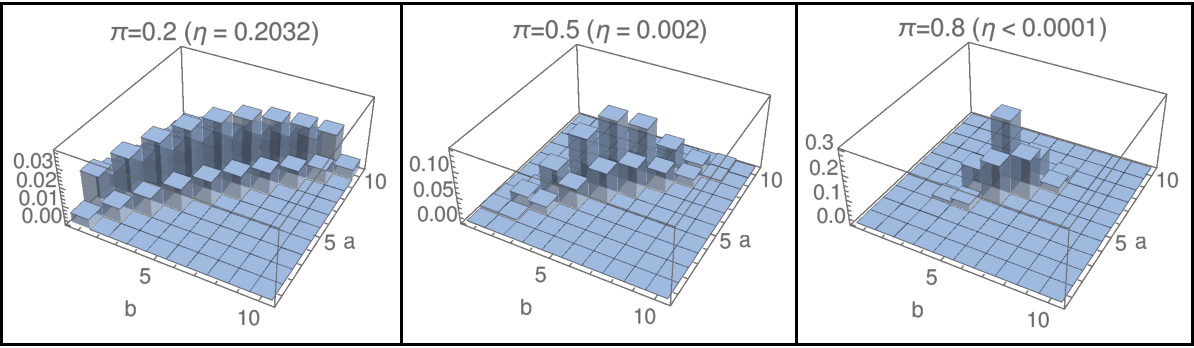
\includegraphics[width=\textwidth]{binom.pdf}
\caption{Distribution of $(A,B)$ in a call auction with $c=0$, $d = 11$, $D=\sum_{i=1}^{d-1} \delta_i V_i$, 
$S=\sum_{i=1}^{d-1} \delta_i W_i$, $V_i \sim \mathrm{Bernoulli}(\pi)$, $W_i \sim \mathrm{Bernoulli}(\pi)$, $0 < i < d$, $\indep(V_1,W_1,V_2,\dots,W_{d-1})$, for various levels of $\pi$. Here, $\eta = \P[B = 0 \vee C = 11]$.}
\label{fig:bin}
\end{center}
\end{figure}


\section{Unit Order Volumes}
\label{sec:cru}

In this subsection, we keep assuming $D\indep S$ to be completely random, but study the special case of the $D$ and $S$ being diffuse (i.e. for any $x\in I$, $D\{x\}=0$, $S\{x\}=0$ w.p.1) and simple (the atoms' weight is always unit). Given these assumptions, by \cite{Kallenberg02}, Theorem 12.10, both $D$ and $S$ are (equivalent to simple) Poisson point processes. Note that, due to our assumption of a finite number of atoms, $D$ and $S$ are fully characterized by 
$\kappa(x)\defined \E K(x)$, $\lambda(x)\defined\E L(x)$, respectively, $x \in I$, with $\kappa(c+)<\infty,\lambda(d-) < \infty$. Let us also recall that we can represent $D=\sum_{i=1}^{N_D} \delta_{V_i}$ where ${N_D}\sim \Po(\kappa(c+))$, the c.d.f. of each $V_i$, $i\in \N$, is $F_D(\bullet)\defined 1-\kappa(\bullet)/\kappa(c+)$, with $\indep (N_D.V_1,V_2,\dots)$ and, similarly, $S=\sum_{i=1}^{N_S} \delta_{W_i}$ where ${N_S}\sim \Po(\lambda(d-))$, the c.d.f. of each $W_i$ is $F_S(\bullet)=\lambda(\bullet)/\lambda(d-)$, and $\indep (N_S.W_1,W_2,\dots)$. 

The following result is a direct consequence of Proposition \ref{th:general}:

\begin{proposition} If $D \indep S$ are (simple) diffuse Poisson, then, for any $c < b \leq a < d$ and $X \subset \N_0$,
\begin{multline}
\P[B<b,A>a,V\in X]=\P[ D[b,a] = 0 ]\P[ S[b,a] = 0]\P[D(a,d)=S(c,b)\in X]\\
= e^{-(\lambda(a)-\lambda(b))}e^{-(\kappa(b)-\kappa(a))}\P[D(a,d)=S(c,b)\in X].
\label{eq:pax}
\end{multline}
\end{proposition}

Applying (\ref{eq:pax}) to single-element $X$'s, we get:
\begin{corollary} For any $c < b \leq a < d$, and $i \in \N_0$,
\begin{multline}
\P[B<b,A>a,V = i] = p(b,a,\{i\}) \\ \defined e^{-(\lambda(a)-\lambda(b))}e^{-(\kappa(b)-\kappa(a))} e^{-\kappa(a)} \frac{\kappa(a)^i}{i!}e^{-\lambda(b)} \frac{\lambda(b)^i}{i!}
 = e^{-\kappa(b)-\lambda(a)} \frac{\kappa(a)^i}{i!}\frac{\lambda(b)^i}{i!}.
\label{eq:pbai}
\end{multline}
\end{corollary}
Further, by taking $X = \N_0$ and using the fact that, for any $\mu\geq 0$ and $\nu \geq 0$, $\P[\Po(\mu)\stackrel{\indep{}}{-}\Po(\nu)=0]=e^{-\mu-\nu}I_{0}(2\sqrt{\mu\nu})$ where $I_0$ is the zero-order modified Bessel function of the first kind (see e.g. \cite{skellam1946frequency}), we get:
\begin{corollary} For any $c < b\leq a < c$,
\begin{equation}
\P[B<b,A>a]=p(b,a,\N_0) \defined e^{-\kappa(b)-\lambda(a)} I_{0}(2\sqrt{\kappa(a)\lambda(b)}).
\label{eq:pba}
\end{equation}
\end{corollary}
\begin{remark}
Equivalently, we can sum (\ref{eq:pbai}) to get,
$$
p(b,a,\N_0)=e^{-\kappa(b)-\lambda(a)}\sum_{i=0}^\infty\frac{(\kappa(a)\lambda(b))^i}{i!i!}.
$$
\end{remark}
As $\P[B\geq A]=0$, (\ref{eq:pbai}) and (\ref{eq:pba}) suffice to evaluate the distributions of $(A,B,V)$, $(A,B)$, respectively.

Assume, until the end of this Section, that $\kappa$ and $\lambda$ are differentiable.

\begin{proposition}
\label{th:abv}
Let either $X = \N_0$ or $X = \{i\}$ for some $i\in \N_0$. Then, for any $Q\in\B([c,d)\times(c,d])$,
\begin{multline}
\P[(B,A,V)\in Q \times X]=\int_{\{(b,a)\in Q: c<b<a<d\}}\gamma(b,a,X)dadb\\
+\charf [0\in X] \left[\int_{\{a:(c,a) \in Q \}}\alpha(a)da
+\int_{\{b:(b,d) \in Q \}}\beta(b)db+\charf[(c,d)\in Q]e^{-\kappa(c)-\lambda(d)}
\right],
\label{eq:pbc}
\end{multline}
where 
$$
\alpha(a)\defined 
\lambda'(a)e^{-\kappa(c)-\lambda(a)},\qquad
\beta(b)\defined-\kappa'(b)e^{-\kappa(b)}{}^{-\lambda(d)},
$$
and
$$
\gamma(b,a,X) = -\frac{\partial}{\partial a\partial b}p(b,a,X).
$$
\end{proposition}

\begin{proof}
See Appendix \ref{app:abv}.
\end{proof}

\begin{corollary}\label{cor:abdens} For any $Q\in\B([c,d)\times(c,d])$,
\begin{multline*}
\P[(B,A)\in Q]=\int_{\{(b,a)\in Q, b \in I, a \in I\}}g(b,a)dadb\\
+\int_{\{a:(c,a) \in Q \}}\alpha(a)da
+\int_{\{b:(b,d) \in Q \}}\beta(b)db+\charf[(c,d)\in Q]e^{-\kappa(c)-\lambda(d)}
\end{multline*}
where 
$$g(b,a)=0,\qquad a<b, $$
and
\begin{multline}
g(b,a)
%= e^{-\kappa(b)-\lambda(a)}
%\left(
%-\kappa'(b)\lambda'(a) \sum_{i=0}^\infty \frac{\lambda(b)^i\kappa(a)^i}{i!i!}
%+\kappa'(a)\kappa'(b) \sum_{i=0}^\infty \frac{\lambda(b)^{i+1}\kappa(a)^i}{(i+1)!i!}
%\right.
%\\
%\left.
%+\lambda'(b)\lambda'(a) \sum_{i=0}^\infty \frac{\lambda(b)^{i}\kappa(a)^{i+1}}{(i+1)!i!}
%-\lambda'(b)\kappa'(a) \sum_{i=0}^\infty \frac{\lambda(b)^{i}\kappa(a)^{i}}{i!i!}
%\right)\\
= e^{-\kappa(b)-\lambda(a)}
\left(
-\left[\kappa'(b)\lambda'(a)+\lambda'(b)\kappa'(a)\right] I_0(2\sqrt{\kappa(a)\lambda(b)})
\right.
\\
\left.
+\left[\kappa'(a)\kappa'(b)
\sqrt{\frac{\lambda(b)}{\kappa(a)}}
+\lambda'(a)\lambda'(b)
\sqrt{\frac{\kappa(a)}{\lambda(b)}}\right] I_1(2\sqrt{\kappa(a)\lambda(b)})
\right), \qquad a \geq b,
\label{eq:gamma}
\end{multline}
where $I_k$ is the modified Bessel function of $k$ -th order of the first kind; we take $\kappa'(a)\sqrt{\frac{\lambda(b)}{\kappa(a)}}=0$ whenever $\kappa(a)=0$ and 
$\lambda'(b)
\sqrt{\frac{\kappa(a)}{\lambda(b)}}=0$ whenever $\lambda(b)=0$.
\end{corollary}



\begin{proof} See Appendix \ref{app:abdens}.
\end{proof}

Furthermore, we evaluate the distribution of $(P,V)$:

\begin{proposition}
Let $X \subseteq \N_0$ be as in Proposition \ref{th:abv}. Then, 
\begin{equation}
\P[P=\undef, V\in X]=\charf[0\in X] [e^{-\kappa(c)}+e^{-\lambda(d)}-e^{-\kappa(c)-\lambda(d)}]\label{eq:pd0}
\end{equation}
and, for any $p\in I$,
\begin{multline}
\P[P<p,P\neq\undef,V\in X]\\=
%\Phi_{\kappa,\lambda}(p)\defined
\int_{c}^{p}\eta(a,a,X)da+\int_{p}^{(2p-c) \wedge d}\eta(2p-a,a,X)da+\charf[0 \in X] [e^{-\kappa(c)-\lambda((2p-c) \wedge d)}-e^{-\kappa(c)}]
\label{eq:pdist}
\end{multline}
where $\eta(b,a,X)=-\frac{\partial}{\partial a} p(b,a,X)$, $b<a$. 
\end{proposition}

\begin{proof}
By Proposition \ref{th:abv}, 
\begin{multline*}
\P[P<p,P\neq\undef,V\in X] =\P[A<d,c<B<2p-A,V\in X]
\\ =\int_{\{a < d\}}\int_{\{ c < b < 2p-a\}}\P_{(B,A,V)}(db,da,X)\\
=\int_{\{c< a < d\}}\int_{\underbrace{\{ c < b < 2p-a, b < a \}}_{\text{$=\emptyset$ for $a \geq 2p-c$}}}\gamma(b,a,X)dbda\\
=\int_c^{(2p-c) \wedge d}\int_c^{a \wedge (2p-a)} \gamma(b,a,X)dbda \\
=\int_c^{(2p-c) \wedge d}[ \eta(a \wedge 2p-a,a,X)da - \eta(c,a,X)]da\\
=\underbrace{\int_c^{(2p-c) \wedge d} \eta(a \wedge 2p-a,a,X)da}_
{=\int_c^p \eta(a, {\dots} + \int_p^{(2p-c) \wedge d} \eta(2p-a,\dots} +
\underbrace{\left[p(c,(2p-c) \wedge d,X)-p(c,c,X)\right]}_{=\charf[0\in X](e^{-\kappa(c)-\lambda((2p-c) \wedge d)}-e^{-\kappa(c)})}
\end{multline*}
(see Appendix \ref{app:abv} for the definition of $p(c,\bullet,X)$).
\end{proof}

\begin{theorem}
(i)
$$
\P[P=\undef]=e^{-\kappa(c)}+e^{-\lambda(d)}-e^{-\kappa(c)-\lambda(d)}.
$$

\noindent (ii) For any $p\in I$ and $v \in \N_0$,
\begin{multline}
\P[P<p,P\neq\undef,V = v]=
%\Phi_{\kappa,\lambda}(p)\defined
\int_{c}^{p}\psi(a,a,v)da \\ +\int_{p}^{(2p-c) \wedge d}\psi(2p-a,a,v)da+\charf[v=0] (e^{-\kappa(c)-\lambda((2p-c) \wedge d)}-e^{-\kappa(c)}),
\label{eq:pdist2}
\end{multline}
where
$$
\psi(b,a,v)=
\begin{cases}
e^{-\kappa(b)-\lambda(a)}\lambda'(a) & v=0,\\
e^{-\kappa(b)-\lambda(a)}\frac{\lambda(b)^v}{v!}\left(\lambda'(a)\frac{\kappa(a)^v}{v!}
- \kappa'(a)\frac{\kappa(a)^{v-1}}{{(v-1)}!}\right) & v>0.
\end{cases}
$$
\noindent (iii) For any $p \in I$,
\begin{multline}
\P[P<p,P\neq\undef]\\=
%\Phi_{\kappa,\lambda}(p)\defined
\int_{c}^{p}\phi(a,a)da+\int_{p}^{2p \wedge d}\phi(2p-a,a)da + [e^{-\kappa(c)-\lambda(2p \wedge d)}-e^{\kappa(c)}],
\label{eq:ppu}
\end{multline}
where 
$$
\phi(b,a)=
e^{-\kappa(b)-\lambda(a)}\left(-\lambda'(a)I_0(2\sqrt{\kappa(a)\lambda(b)})+\kappa'(a)\sqrt{\frac{\lambda(b)}{\kappa(a)}}I_1(2\sqrt{\kappa(a)\lambda(b)})\right)
$$
taking $\kappa'(a)\sqrt{\frac{\lambda(b)}{\kappa(a)}}=0$ whenever $\kappa(a)=0$.

\noindent (iv) For any $v\in \N_0$,
$$
\P[V=v]\\=
%\Phi_{\kappa,\lambda}(p)\defined
\int_{c}^{d}\psi(a,a,v)da + \charf[v = 0] e^{-\lambda(d)}.
$$
\end{theorem}

\begin{proof} (i) follows from (\ref{eq:pd0}), (ii) and (iii) follow from (\ref{eq:pdist}), to get (iv), it suffices to take the limit $p\rightarrow d$ in (\ref{eq:pdist}).
\end{proof}

\begin{corollary} \label{cor:dens}
 $P$ is absolutely continuous w.r.t. $\delta_\undef+\ell((c,d))$, where $\ell$ denotes the Lebesgue measure, with density 
\begin{equation}
f(\undef)=e^{-\kappa(c)}+e^{-\lambda(d)}-e^{-\kappa(c)-\lambda(d)},\qquad 
f(p)=2 \int_p^{2 p \wedge d} g(2p-a,a) da.
\label{eq:pdens}
\end{equation}
\end{corollary}

\begin{proof} See Appendix \ref{app:dens}.
\end{proof}




 

\section{Random Order Volumes}
\label{sec:crr}

In the present Section, we release the assumption of unit weights, still assuming that $D\indep S$ are diffuse complete random, but allowing for (i.i.d.) random weights with the same distribution for buy-- and the sell orders. Under these assumptions, the locations of the $D$'s and $S$'s atoms form a (diffuse) Poisson point processes, which we denote $D_g$, $S_g$, respectively.

\def\cpo{\mathrm{CPo}}

\begin{theorem} Let $D \indep S$, let $D_g$, $S_g$ be diffuse Poisson and let the weights of the atoms be i.i.d., following a distribution $\L$ such that $\L(-\infty,0]=0$. Then, for any $c < b \leq a < d$,
\begin{equation}
\label{eq:pbcp}
\P[B<b] = \P[\mathcal{C}(\kappa_g(b),\lambda_g(b),\L)\leq 0],
\end{equation}
\begin{equation}
\label{eq:pacp}
\P[A<a] = \P[\mathcal{C}(\kappa_g(a),\lambda_g(a),\L)< 0],
\end{equation}
and
\begin{multline*}
\P[B<b,A<a] = \P[\mathcal{C}(\kappa_g(b),\lambda_g(b),\L)\leq 0]
\\
- e^{-(\lambda_g(a)-\lambda_g(b))}e^{-(\kappa_g(b)-\kappa_g(a))}\P[\mathcal{C}(\kappa_g(a),\lambda_g(b),\L)=0];
\end{multline*}
here, $\kappa_g(\pi)=\E D_g[\pi,d)$, $\lambda_g(\pi)=\E S_g(c,\pi]$, $\pi \in I$, and $\mathcal{C}(\kappa,\lambda,\L)$ is the Compound Poisson distribution with intensity $\kappa+\lambda$ and embedded distribution $\frac\kappa{\kappa+\lambda} \L + \frac\lambda{\kappa+\lambda} \L^-$ where $\L^-$ is  the $\L$'s negative version (i.e. $\L(x,\infty)=\L^-(-\infty,-x)$, $x \in \R$).
\end{theorem}
\begin{proof}
The assertion follows from Proposition \ref{cor:cr}, using the fact that the convolution of two compound Poisson distributions is compound Poison with properly weighted mixed embedded distribution.
\end{proof}

%https://www.sciencedirect.com/science/article/abs/pii/0167637784900087

\noindent In the following Theorem, we evaluate the asymptotic distributions of the clearing price and the bounds of the traded volume.

\begin{theorem} \label{th:asymp} Let $\kappa_0,\lambda_0:I\rightarrow \R_+$ be strictly increasing, decreasing, respectively, and differentiable. Let $\L$ be distribution with $\L(-\infty,0]=0$ having a finite third moment. For any $n \in \N$, let $P_n,B_n,A_n,\dots$ be the clearing price, lower price limit, upper price limit, etc., in a call auction with independent compound Poisson order books defined by $\kappa_g = n \kappa_0$ and $\lambda_g = n\lambda_0$ and the atoms' weight distribution $\L$. Let $p$ be the solution of the equation $\kappa_0(p)= \lambda_0(p)$. Then\\
(i) $$P_n\stackrel{P}\longrightarrow p$$
(ii)
\begin{multline*}
\sqrt{n}(P_n-p) \stackrel{d} \longrightarrow \ND\left(0,v_gr_\L\right), 
\\ 
v_g \defined \frac{\kappa_0(p)+\lambda_0(p)}{(\lambda_0'(p)-\kappa_0'(p))^2}=\frac{2\kappa_0(p)}{(\lambda_0'(p)-\kappa_0'(p))^2}
=
\frac{2\lambda_0(p)}{(\lambda_0'(p)-\kappa_0'(p))^2},
\qquad
r_\L = \frac{\E \L^2}{(\E \L)^2},
\end{multline*}
where  $\E\L$ and $\E\L^2$ are the $\L$'s expectation, (non-central) second moment, respectively.\\
(iii) 
$$W^-_n \leq V_n \leq W^+_n,\qquad 
W^-_n \defined V_n^-(p),\qquad W_n^+ \defined V_n^+(p),$$
with
$$
\frac{1}{\sqrt{n}}(W_n^--n \mu)\stackrel{d}\longrightarrow \mathcal{M}_{w}, 
\qquad 
\frac{1}{\sqrt{n}}(W_n^+-n \mu)\stackrel{d}\longrightarrow \mathcal{M}^{w};
$$
$$
\mu = \kappa_0(p) \E\L = \lambda_0(p) \E\L, \quad
w = 
\kappa_0(p) \E \L^2= \lambda_0(p) \E \L^2,
$$
where $\mathcal{M}_w$, $\mathcal{M}^w$, are the distributions of the minimum, maximum, respectively, of two independent $\ND(0,w)$ random variables. In particular
$$
\P\left[ \frac{1}{\sqrt{n}}(W^-_n-n \mu)  < x
\right] = 1-\left(1-\varphi\left(\frac{x}{\sqrt{w}}\right) \right)^2,
$$
$$
\P\left[ \frac{1}{\sqrt{n}}(W^+_n-n \mu) < x
\right] = \varphi\left(\frac{x}{\sqrt{w}}\right)^2,
$$
where $\varphi$ is the standard normal c.d.f.
\end{theorem}

\begin{proof} See Appendix \ref{app:asymp}.
\end{proof}


\begin{corollary}
If, in Theorem \ref{th:asymp}, $\L = \delta_1$ (i.e., the volumes are deterministic and unit), then the Theorem holds with 
$v_g = \frac{2\kappa(p)}{[\lambda'(p)-\kappa'(p)]^2}$, $r_L=1$, $\mu = w = \kappa(p)=\lambda(p)$.
\end{corollary}

\paragraph*{Numerical Illustration.}
Once the trading intensities are high enough, we can represent $P=P_n$, $V^-(p)=V_n^-(p)$ and $V^+(p)=V_n^+(p)$ for some $n$ and approximate
$$
P \quad \dot \sim \quad 
\ND\left(p,\frac{2\kappa_g(p)\E\L^2}{(\kappa'_g(p)-\lambda'_g(p))^2(\E \L)^2} \right ),
$$
and
$$
W^- \leq V \leq W^+,
$$
where
$$
\P\left[ W^-  < x
\right] \doteq 1-\left(1-\varphi\left(\frac{\kappa_g(p)\E \L+x}{\sqrt{\kappa_g(p)\E \L^2}}\right) \right)^2
$$
$$
\P\left[ W^+ < x
\right] \doteq \varphi\left(\frac{\kappa_g(p)\E \L+x}{\sqrt{\kappa_g(p)\E \L^2}}\right)^2
$$
$x \in I$. In Figure \ref{fig:il}, we illustrate the accuracy of these approximations for various levels of trading intensity: we assume that order volumes and intensities are multiples of linear functions, different for demand and supply. It can be seen that the approximations are nearly perfect, once there are tens of orders on both sides (recall that the expected number of buy and sell orders equals $\kappa(c+)$, $\lambda(d-)$, respectively.

\begin{remark} As, by the Schwarz inequality, $r_\L \geq 1$, with the minimum achieved by $\L = \delta_1$, we see that taking randomness of the order volumes into account leads to higher (asymptotic) variance of both the price and the volume bounds in comparison with the usual approximation of the volumes by their mean values (normed to one). 
\end{remark}

Next, we compare our asymptotic result with that of \cite{derksen2020clearing}:

\begin{remark} Consider
$$
D=\sum_{i=1}^{N_D} \delta_{D_i}, \qquad S=\sum_{i=1}^{N_S} \delta_{S_i}
$$
where $\E N_D=(1-\alpha)n$, $\E N_S=\alpha n$ for some $\alpha \in (0,1)$ and $n\in \N$,  $D_i$, $i\in\N$, being i.i.d. with strictly increasing absolutely continuous c.d.f. $F_D$, and $S_i$, $i\in \N$ being i.i.d. with strictly increasing a.c. c.d.f $F_S$, such that all the variables are mutually independent.

Once $N_S$ and $N_D$ are Poisson, $D$ and $S$ are Poisson processes determined by 
$$
\kappa(x)=n (1-\alpha) (1-F_D(x)), \qquad \lambda(x)=n \alpha F_S(x),
$$
and, by Theorem \ref{th:asymp},
$$
\sqrt{n}(P_n-p) \rightarrow_n \ND(0,v), 
\qquad 
v=\frac{ 2 \alpha F_S(p) }{[(1-\alpha)f_D(p)+\alpha f_S(p)]^2}.
$$
 

If, instead, $N_D=(1-\alpha) n$ and $N_S = \alpha n$ are deterministic, we have, by Theorem 3.1 of \cite{derksen2020clearing}, that 
$$
\sqrt{n}(P_n-p) \rightarrow_n \ND(0,\tilde v), 
\qquad 
\tilde v=\frac{ \alpha [F_D(p)+ (1-F_S(p))]F_S(p)}{[(1-\alpha)f_D(p)+\alpha f_S(p)]^2}
$$
By comparison of the asymptotic variances we see that assuming random order numbers increases the price variance significantly compared with only using their expectations. 
\end{remark}


\begin{figure}
\begin{center}
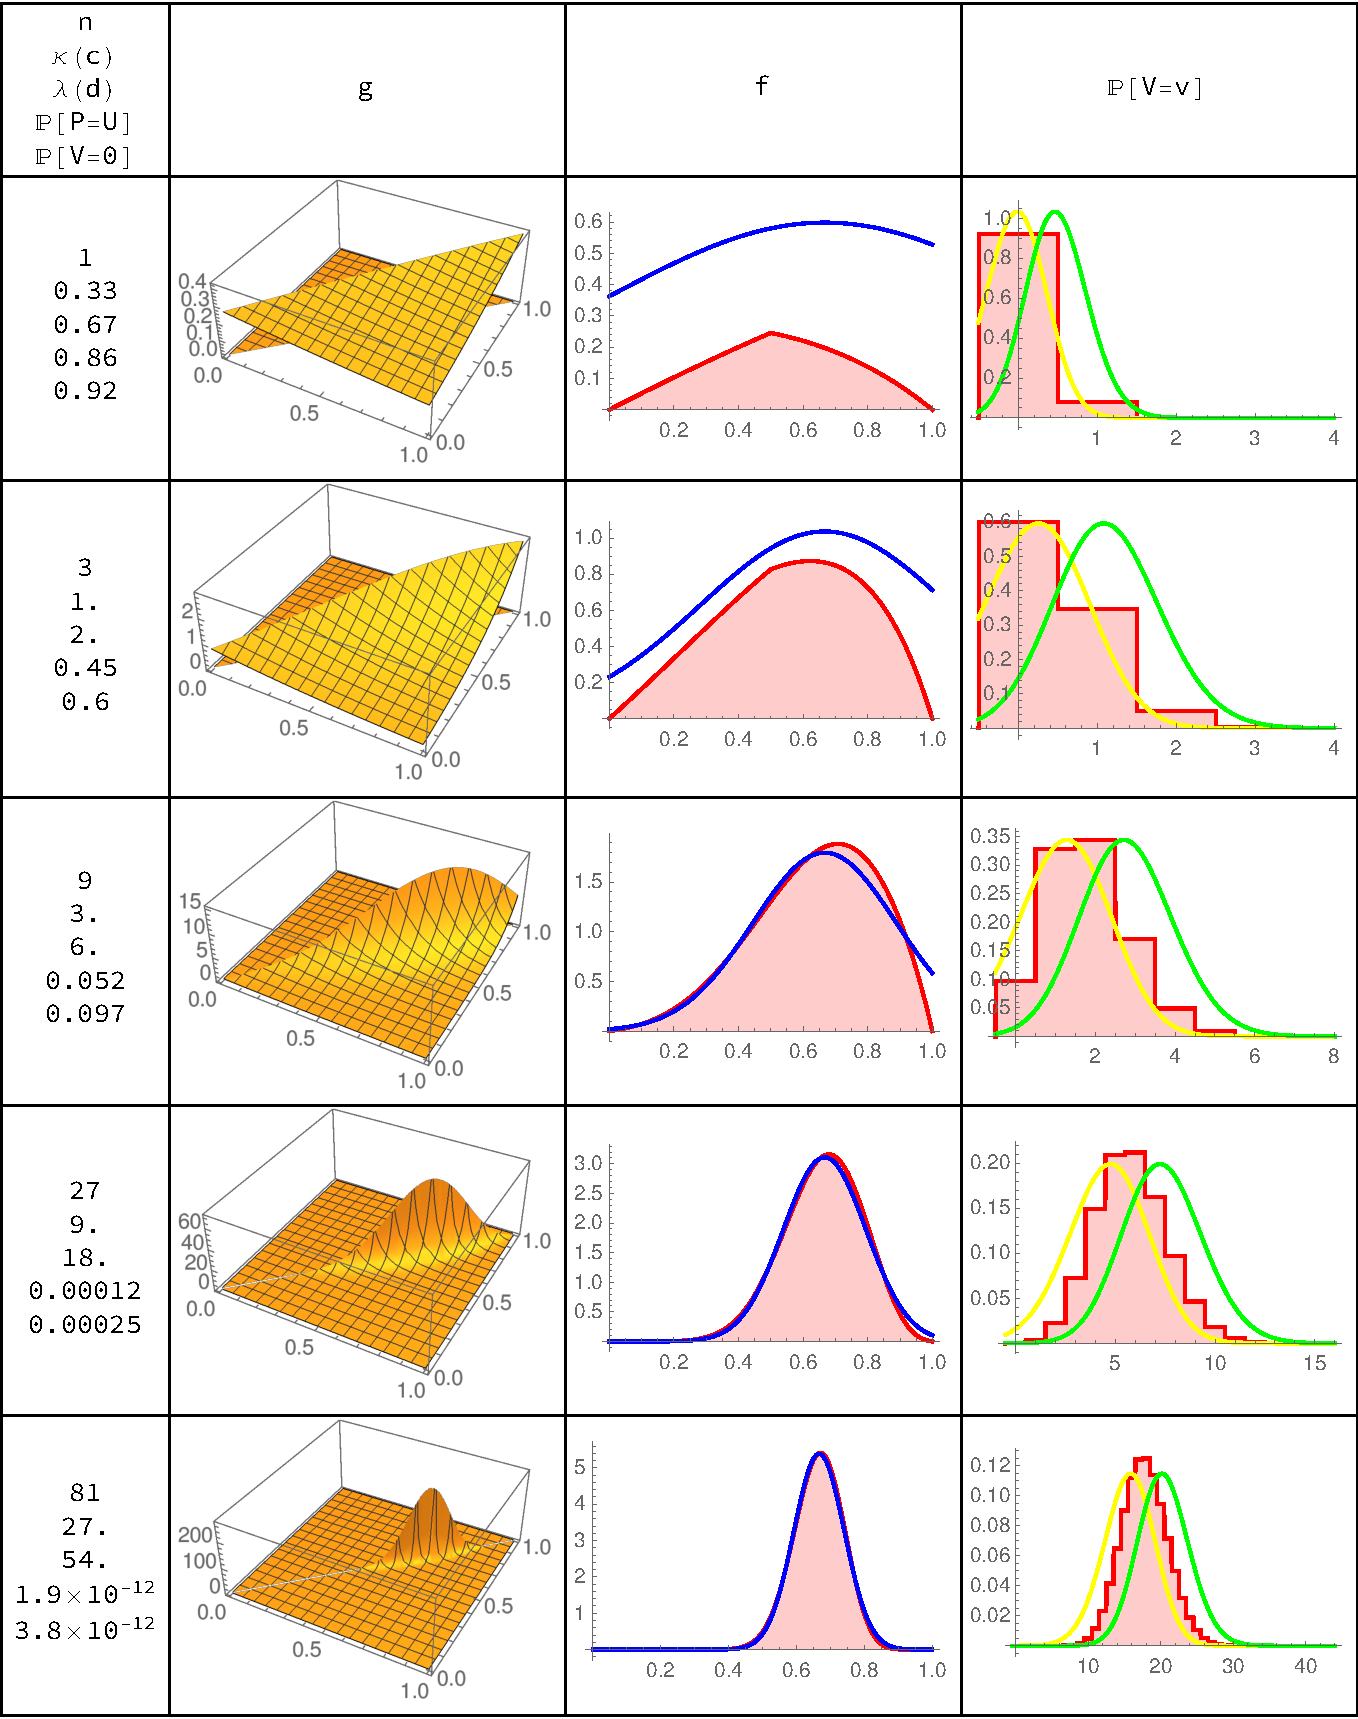
\includegraphics[width=\textwidth]{illust.pdf}
\caption{Distribution of $(A,B)$, $P$ and $V$ for $\kappa(a)=n \frac{2}{3}(1-a)$, $\lambda(b)=n \frac{1}3 b$ and unit order volumes. Blue, normal approximation of $P$, yellow, normal approximation of $W^-$, green, normal approximation of $W^+$. }
\label{fig:il}
\end{center}
\end{figure}

\section{Conclusions}

We have thoroughly studied a natural stochastic model of call auction. We have described both the exact and the asymptotic distributions in various special cases of this model. The next natural step could be to describe the dynamics of repeated call auctions, suggested by \cite{budish2015high}, and compare it with that of the continuous double auction.

\paragraph*{Acknowledgments} This work was supported by grant No. GA19-11062S from the Czech Science Foundation. Computational resources were partially provided by the ``eInfrastruktura CZ'' (e-INFRA CZ LM2018140) project supported by the Ministry of Education, Youth and
Sports of the Czech Republic

%\bibliographystyle{APT}
\footnotesize
%\bibliography{../../smid}
\documentclass{aptpub}
\usepackage{graphicx}
\usepackage{hyperref}
\authornames{\v Sm\'\i d, Kub\v ena} % insert the authors here for use in running head. If three or more authors please use (for example) M.~YARROW {\it et al}. Author names should follow the same M.~YARROW format and if two authors, separate by 'AND'.
\shorttitle{Distribution of Call Auction} % insert short title here for use in running head

% Put any of your own definitions here.

%\numberwithin{equation}{section}  % If you number theorems, etc. within sections,
                                   % then please uncomment this line to number
                                   % equations with sections too.

\global\long\def\P{\mathbb{P}}%
\global\long\def\N{\mathbb{N}}%
\global\long\def\U{\mathbb{U}}%
\global\long\def\E{\mathbb{E}}%
\global\long\def\R{\mathbb{R}}%
\global\long\def\G{\mathcal{G}}%
\global\long\def\g{\mathbb{\Pi}}%
\global\long\def\F{\mathcal{F}}%
\global\long\def\S{\mathbb{S}}%
\global\long\def\Q{\mathcal{Q}}%
\global\long\def\B{\mathcal{B}}%
\global\long\def\ND{\mathcal{N}}%
\global\long\def\XX{\mathcal{X}}%
\global\long\def\indep#1{{\perp\hspace{-2mm}\perp}#1}%
\global\long\def\L{\mathcal{L}}%
\global\long\def\var{\mathrm{var}}%
\global\long\def\cov{\mathrm{cov}}%
\global\long\def\charf{\mathbf{1}}%
\global\long\def\d{\mathrm{d}}%
\global\long\def\M{\mathcal{M}}%
\global\long\def\Exp{\mathrm{Exp}}%
\global\long\def\Uniform{\mathrm{U}}%
\global\long\def\eqd{\stackrel{d}{=}}%
\global\long\def\eqas{\stackrel{a.s.}{=}}%
\global\long\def\X{\mathcal{X}}%
\global\long\def\supp{\mathrm{support}}%
\global\long\def\H{\mathcal{H}}%
\global\long\def\Z{\mathcal{Z}}%
\global\long\def\as{\qquad a.s.}%
\global\long\def\on{\qquad\text{on }}%
\global\long\def\C{\mathcal{C}}%
\global\long\def\barxi{\overline{\xi}}%
\global\long\def\Po{\mathrm{Po}}%
\global\long\def\Bi{\mathrm{Bi}}%
\global\long\def\Be{\mathrm{Be}}%
\global\long\def\defined{\stackrel{\text{def}}{=}}%
\global\long\def\barA{\overline{A}}%
\global\long\def\A{\mathcal{A}}%
\global\long\def\barx{x}%
\global\long\def\barX{TBD}%
\global\long\def\last{\ell}%
\global\long\def\bary{y}%
\global\long\def\barz{z}%
\global\long\def\DD{\mathcal{D}}%
\global\long\def\undef{\mathfrak{U}}


\begin{document}%\recd{}{}%Do not alter this line.

\title{Distribution of Price and Volume in Call Auction} % insert title - use `\\ if it requires more than one line.

\authorone[Czech Academy of Sciences]{Martin   \v Sm\'\i d} 
%Affiliation is just the name of your university or institution, for example 'University of Sheffield'. Author names should be of the form 'Mark Yarrow'. 
%Authors should be ordered alphabetically subject to the convention in that particular authors country. For example 'Remco van der Hofstad' would be listed under 'H' as is standard in the Netherlands. 
\authortwo[Czech Academy of Sciences]{Ale\v s Anton\`\i n Kub\v ena} 

%Please use the following format for addresses and emails. The APT office will sort this out after you submit your files.
\addressone{Institute of Information Theory and Automation of the CAS. Pod Vod\' arenskou v\v e\v z\'\i 4, Praha 8, 182 00, Czech Republic,
              Tel.: +420-2-66052400} % Your postal address goes here.
\emailone{smid@utia.cas.cz} %Authors email goes here.

\begin{abstract}

We describe exact and asymptotic distributions of the settlement price and the traded volume in call auction. On top of existing results, we allow completely random order books and random order volumes. We show that approximating random order volumes and/or order numbers by constants leads to a significant underestimation of both the settlement price and the traded volume variances. We also demonstrate a rapid speed of convergence of the asymptotic distributions to the exact ones. 
%, which is a trading mechanism accumulating demand and supply for some time period and then settling them for a price maximizing the traded volume. 

\end{abstract}

\keywords{call auction, settlement price, traded volume, exact distribution, asymptotic distribution}%insert keywords separated by a semicolon. You should avoid including keywords which also appear in the title.

\ams{91G15}{60G57}% insert the primary 2020 Maths Subject Classification number in the first bracket
		% and the secondary ams number(s) in the second bracket
		% e.g. \ams{60E20}{49G03;49F10}
		%Maximum of three in each, ideally one or two in each primary and secondary.
		%codes found here ``https://mathscinet.ams.org/msnhtml/msc2020.pdf''


\section{Introduction}

Yet trading on today's financial markets is mostly continuous \cite{friedman2018double}, the days of {\em call auction} -- a simpler trading mechanism in which the price is being determined at fixed time instants rather than after each order arrival -- are far from being numbered. Call auctions are used to determine closing and opening prices in electronic markets \cite{toke2015exact}, and there are even suggestions to replace continuous trading by frequent batch auctions to avoid time arbitrage \cite{budish2015high}. 

In comparison with its continuous counterpart, relatively little scientific attention has been paid to call auction. Seminal work \cite{mendelson1982market} studies its simple model with unit order volumes and uniform limit price distributions. Paper \cite{toke2015exact}  generalizes these results, analytically describing the exact and asymptotic marginal distributions of traded volume and the price limits given a general (absolutely continuous) limit price distribution, which is the same for buy and sell orders, but an imbalance of arrival rates is allowed. More recent work \cite{derksen2020clearing} allows for differently distributed buy-- and sell limit prices; moreover, a (deterministic) excess liquidity may exist. An analytical formula is derived for the exact {\em conditional joint} distribution of the clearing price and the traded volume given the order numbers, as well as an asymptotic formula for the {\em unconditional} distribution of the clearing price given that the {\em deterministic} numbers of orders grow to infinity. 

We present more general results as we assume random order volumes and
derive general formulas for the {\em exact unconditional} joint distributions of price limits and, given unit order sizes, also for the {\em exact unconditional} joint distribution of the price limits and the traded volume (Section \ref{sec:call}). 

Further, we derive more detailed formulas for the case in which the order books (i.e. the collections of orders of the same type) are completely random (i.e. Poisson or having discrete limit prices with independent volumes, Section \ref{sec:cr}). In the special case of unit order sizes, we describe the exact joint distribution of the price and the traded volume (Section \ref{sec:cru}) and, for the general case, we derive asymptotic (marginal) distributions of the price and the bounds for the traded volume (Section \ref{sec:crr}). Finally, we numerically illustrate that the convergence of the asymptotic distributions to their exact counterparts is rapid.

It turns out that both the randomness of the order numbers and the randomness of the traded volumes matter, significantly increasing the price (asymptotic) variance compared to the approximations assuming unit orders \cite{mendelson1982market,toke2015exact,derksen2020clearing} and/or deterministic order numbers \cite{derksen2020clearing}.




\section{Call Auction}
\label{sec:call}

We first describe the call auction. Let $I=(c,d)$, $c\in\R_{-\infty}$, $d\in\R_{\infty}$ be an open
interval of possible prices and let $D,S$ be atomic random measures with finitely many atoms,
describing the order books. In particular, each atom of $D$/$S$ represents a buy/sell
limit order with the limit price corresponding to the atom's location and the ordered/offered volume corresponding to its weight.
Let us recall that a buy/sell limit order is a commitment to buy/sell a specified {\em volume} for no more/no less than a specified {\em limit price}.

There are more ways to choose the clearing price. Usually, one of the prices is chosen that maximizes the volume traded. In this work, we take the average value for which the demand and supply curves actually intersect as the clearing price.

\begin{figure}
\begin{center}
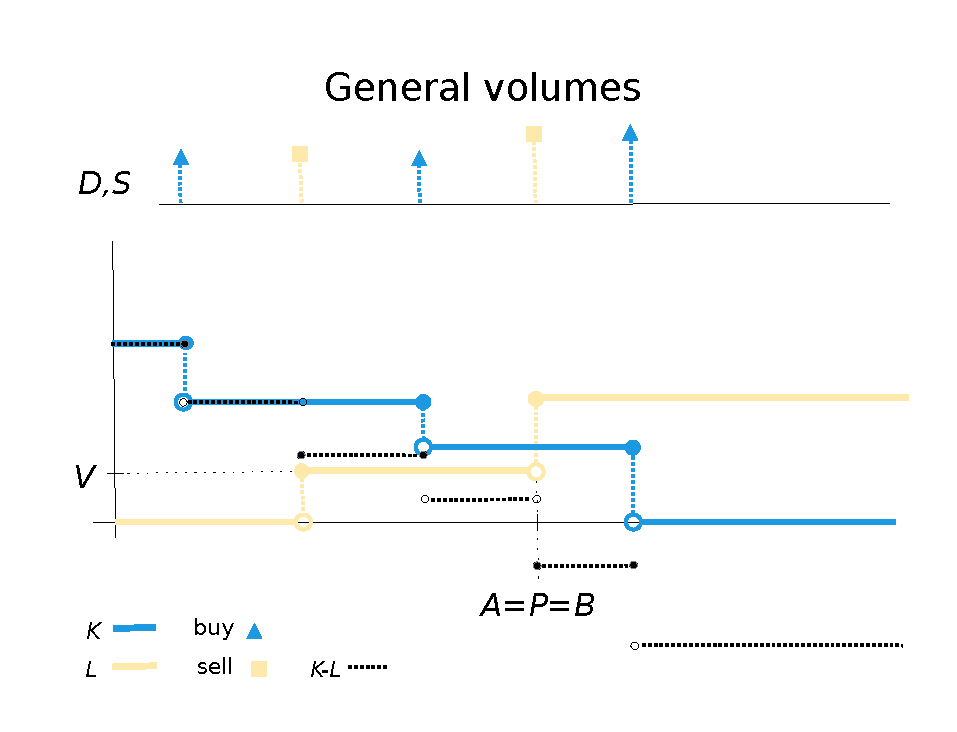
\includegraphics[width=6cm]{nuob.pdf}
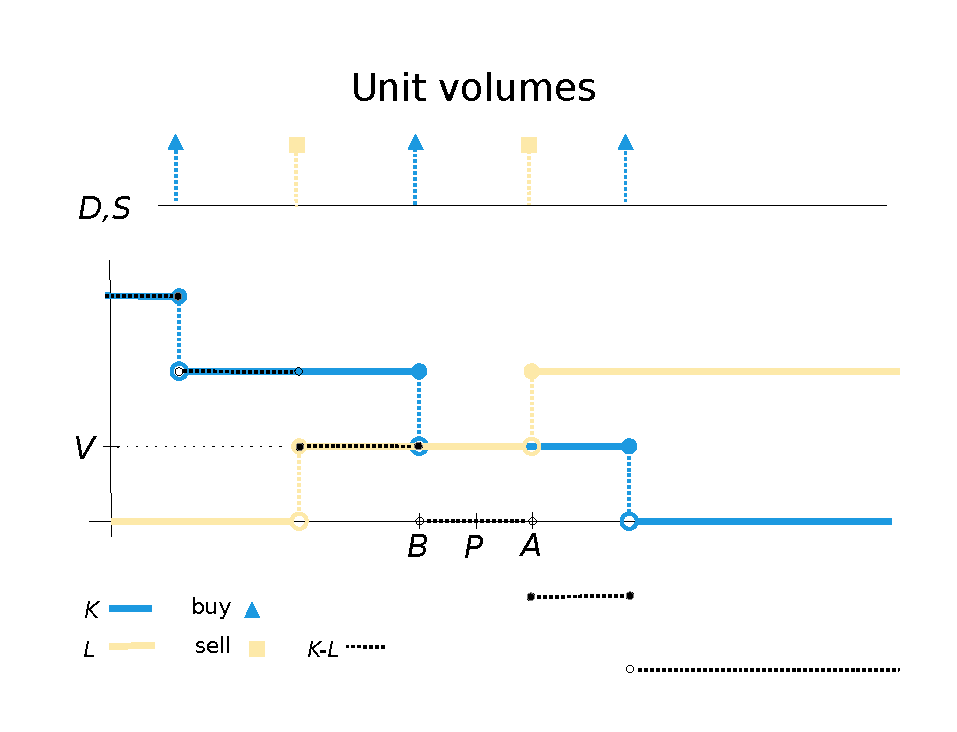
\includegraphics[width=6cm]{ob.pdf}
\end{center}
\caption{Call auction with general order volumes (left) and unit order volumes (right), respectively.}
\label{fig:ob}
\end{figure}

Formally, denoting $K(\pi)=D[\pi,d)$ and $L(\pi)=S(c,\pi]$, $\pi\in I$,
(the demand/supply curves), the maximum traded volume is 
\begin{equation}
V = \max_{p \in I} V^-(p),\qquad V^-(p) \defined K(p) \wedge L(p),
\label{eq:vdef}
\end{equation}
and, further denoting $A=\inf\{\pi\in I:K(\pi)<L(\pi)\}$ and $B=\sup\{\pi\in I:K(\pi)>L(\pi)\}$ 
the price limits,
the clearing price is 
$$P=\begin{cases}\frac{B+A}{2} & A \neq d, B \neq c,
\\\undef & \text{otherwise},
\end{cases}
$$
where $\undef\notin\R$ denotes an undefined price (note, however, that, in some cases with $V=0$, $P$ might be defined). See Figure \ref{fig:ob} for an illustration. 

Our setting covers both the case of continuous limit prices (atoms of $D$ and $S$ may find themselves anywhere in $I$) and the case of discrete prices (atoms of $D$ and $S$ can find themselves only in discrete points, corresponding to price ticks). Note that we do not require the weights (volumes) to be integers. 

Next, we show that $P$ indeed maximizes the traded volume, and, as the traded volume is generally difficult to handle, we introduce its bounds.

\begin{proposition}
(i) 
$$V=\begin{cases} V^-(P) & A \neq d, B \neq c
\\0 & \text{otherwise}
\end{cases}
$$
(ii) For any $p\in I$, $V^-(p) \leq V \leq V^+(p)$ where $V^+(p) = K(p) \vee L(p)$.
\end{proposition}

\begin{proof} (i) When $A = d$ or $B=c$, the assertion is trivial. Let $A \neq d, B \neq c$.
First, note that $V^- = L$ on $(c,A)$ and $V^- = K$ on $(B,d)$. 

Thus, once $B<A$, $V^-$ is non-decreasing on $(c,A)$ and non-increasing on $(B,d)$, which implies that it is constant on $(B,A)$ and  its maximum happens (also on) $(B,A)$, specially in $P$.


If $A=B=P$, then, due to monotonicity, at least one of the following values is equal to $\sup V^-$: $V^-(P-)[=L(P-)],V^-(P+)[=K(P+)]$ or 
$V^-(P)[=K(P) \wedge L(P)=K(P-) \wedge L(P+)]$.
If $K(P-) \geq L(P+)$, then $V^-(P)=L(P+)\geq L(P-)=V^-(P-)$, so only two candidates remain: $V^-(P)[=L(P+)]$ and  $V^-(P+)[=K(P+)]$; however, as the former is strictly greater from the definition of $A$, we proved that the maximum occurs at $P$. Analogously, we can show that $V^-$ is maximized in $P$ if $K(P-) \leq L(P+)$.

\noindent (ii) The first inequality follows directly from (\ref{eq:vdef}). The second one holds trivially if $K(p)=L(p)$ or $V=0$. If $V > 0$ and $K(p)<L(p)$, then $c < B \leq A < p$ hence $P < p$ and, by (i), $V=V^-(P)=K(P) \wedge L(P) \leq L(P) \leq L(p) \leq L(p) \vee K(p)$; similarly for $K(p)>L(p)$.
\end{proof}



\noindent Next we present general formulas for the distribution of random vector $(A,B)$. 

\begin{proposition} \label{th:gen} Let $c<b\leq a \leq d$, put $N_\pi \defined D[\pi,d)-S(c,\pi)$, $\pi \in I$. Then\\
(i) $\P[B<b] = \P[N_b \leq 0]$,\\
(ii)  $\P[A<a] = \P[N_a < 0]$,\\
(iii) $\P[B<b,A<a]=\P[N_b\leq 0]-\P[D[a,d)=S(c,b),S[b,a)=0,D[b,a)=0].$\\
\end{proposition}

\begin{proof} Denote $\Delta = K-L$. As $\Delta$ is a non-decreasing step function, we have
$$[B<b] = [\sup\{\pi\in I:\Delta(\pi)>0\} < b] = [\Delta(b-)\leq 0]$$
and
$$
[A<a] = [\inf\{\pi\in I:\Delta(\pi)< 0 \} < a]
= [\Delta(a-)< 0] 
$$
which proves (i), (ii), respectively because $N_\pi=\Delta(\pi-)$, $\pi \in I$. Further,
\begin{multline*} 
[B<b,A<a] = [\Delta(b-)\leq 0,\Delta(a-)< 0] = [\Delta(b-) < 0] \cup [\Delta(b-) = 0, \Delta(a-)-\Delta(b-) < 0]
\\
=[\Delta(b-) < 0] \cup ( [\Delta(b-) = 0] \setminus E)
\qquad E \defined [\Delta(b-) = 0,\Delta(a-)-\Delta(b-) = 0].
\end{multline*}
As the union is discrete and the difference is proper, we have
$$
\P[B<b,A<a] = \P[\Delta(b-)\leq 0]-\P E = \P[N_b\leq 0]-\P E.
$$
Employing the monotonicity of $\Delta$ and the fact that it jumps at any atom of $D$ or $S$,  we further get
$$
E = [\underbrace{\Delta(b-)}_{=D[b,d)-S(c,b)}=0,S[b,a) = 0, D[b,a)=0], 
$$
which is equivalent to
$$
E=[D[a,d)=S(c,b),S[b,a)=0,D[b,a)=0]
$$
proving (iii).
\end{proof}


\noindent If the offered/ordered volumes are always unit and the atoms of $D$ and $S$ do not coincide w.p.1, then  $K-L$ has unit jumps (down) w.p.1, implying that $B < A$ and, consequently, $V=K(P)=L(P)$ whenever $P\neq \undef$ (note that $V=0$ if $P=\undef$), so we are able to evaluate the joint distribution of $(A,B,V)$:

\begin{proposition} \label{th:general} Let the atoms of $D+S$ have unit weights w.p.1. Then, for any $c< b \leq a < d$ and any $X \subseteq \N_0$,
\begin{equation}
\P[B<b,A>a,V\in X]=\P[ D[b,a] = 0, S[b,a] = 0, D(a,d)=S(c,b)\in X].
\label{eq:pbax}
\end{equation}
\end{proposition}

\begin{proof} Denote $p = \frac{a+b}2$. As $\Delta \defined K-L$ is non-increasing, we have
\begin{multline*}
[B < b,A > a] = [\sup\{\pi\in I:\Delta(\pi)>0\} < b \leq a < \inf\{\pi\in I:\Delta(\pi)< 0 \} ]
\\= [\Delta(b-)\leq 0,\Delta(a+)\geq 0] = [\Delta(b-) = 0,\Delta(a+) = 0]
= [\Delta(b-)=0, \Delta(b-)-\Delta(a+)=0]
\\=[D[b,d)=S(c,b), D[b,a] = 0, S[b,a] = 0]
=[ D(a,d)=S(c,b), D[b,a] = 0, S[b,a] = 0].
\end{multline*}
Therefore and as $B<b,A>a \Rightarrow V=D(a,d)=S(c,b)$, we get (\ref{eq:pbax}).

\end{proof}



\section{Completely Random Order Books}
\label{sec:cr}

Next, we discuss the special case where $D$ and $S$ are mutually independent and completely random. Recall that a random measure $M$ on $(I, \B(I))$ is {\em completely random} if, for any disjoint $S_1,\dots,S_k\in \B(I)$, $MS_1,\dots,MS_k$ are independent. Note also that the class of completely random measures embraces (marked) diffuse Poisson point processes (viewed as measures) as well as the measures with fixed atoms with mutually independent weights (usable in discrete price settings). In fact, any completely random purely atomic measure is a sum of a measure of the former type and a measure of the latter type (see \cite{daley03}, Theorem 10.1.III). 

It is well known (see, e.g. \cite{daley03}, 2.1.6 and 10.1.VI) that a measure $M=\sum_{i=1}^N W_i \delta_{U_i}$, where $\delta_x$ is the Dirac measure concentrated in $x$, $N$ is Poisson, $U_i$'s are i.i.d,, $W_i$'s are i.i.d. and $N,U_1,W_1,U_2,\dots$ are mutually independent (the setting studied by \cite{toke2015exact}) is completely random, but stops to be so once $N$ becomes deterministic (which is the case studied by \cite{derksen2020clearing}); consider $M=\delta_U$ with random $U$, for instance. Further note that, once the process of order arrivals is Poisson and the orders are possibly canceled with a fixed rate, dependent only on the limit price, then the process of valid orders is still Poisson and the corresponding order book is still completely random and Poisson (see, e.g. \cite{smid16estimation}, Example 2.3).


The following result stems directly from Proposition \ref{th:gen}:

\begin{proposition}
\label{cor:cr} If $D \indep S$ and both $D$ and $S$ are completely random, then, for any $c < b \leq a \leq d$,
$$\P[B<b,A<a] = \P[N_b\leq 0]-\P[D[a,d)=S(c,b)]\P[S[b,a)=0]\P[D[b,a)=0]$$
\end{proposition}

\begin{example} Assume discrete prices: $c=0$, $d \in \N$, $D=\sum_{i=1}^{d-1} \delta_i V_i$, 
$S=\sum_{i=1}^{d-1} \delta_i W_i$ where $V_i \sim \mathrm{Bernoulli}(\pi)$, $W_i \sim \mathrm{Bernoulli}(\pi)$, $0 < i < d$, with $V_1,W_1,V_2,\dots,W_{d-1}$ independent. Then
$$
\P[A=d]=\P[B=c]=(1-\pi)^{d-1}, \qquad  \P[A=d, B=c]=(1-\pi)^{2d-2},
$$
and, by Proposition \ref{cor:cr}, for any $0 < a \leq b < d$,
\begin{multline*}
\P[B< b, A < a]
%\\ = \P[D[b,d)-S(c,b)\leq 0]-\P[D[a,d)=S(c,b)] \P[S[b,a)=0]\P[D[b,a)=0]
=
\P[\Bi(d-b,\pi)\stackrel{\indep{}}-\Bi(b-1,\pi)\leq 0] \\ -\P[\Bi(d-a,\pi)\stackrel{\indep{}}-\Bi(b-1,\pi)=0]
\P[\Bi(a-b,\pi)=0]\P[\Bi(a-b,\pi)=0] \\
= \sum_{k=-(b-1)}^0 q_{d-b,b-1,\pi}(k)-q_{d-a,b-1,\pi}(0)(1-\pi)^{2a-2b}
\end{multline*}
where $q_{m,n,\pi}(k) \defined \P[\Bi(m,\pi)\stackrel{\indep{}}-\Bi(n,\pi)=k]$ for any $m,n,\pi,k$. Using this and the fact that $\P[B>A]=0$ we can obtain the distribution of $(A,B)$. In Figure \ref{fig:bin}, this distribution is plotted for $d=11$ and various values of $\pi$.
\end{example}

\begin{figure}
\begin{center}
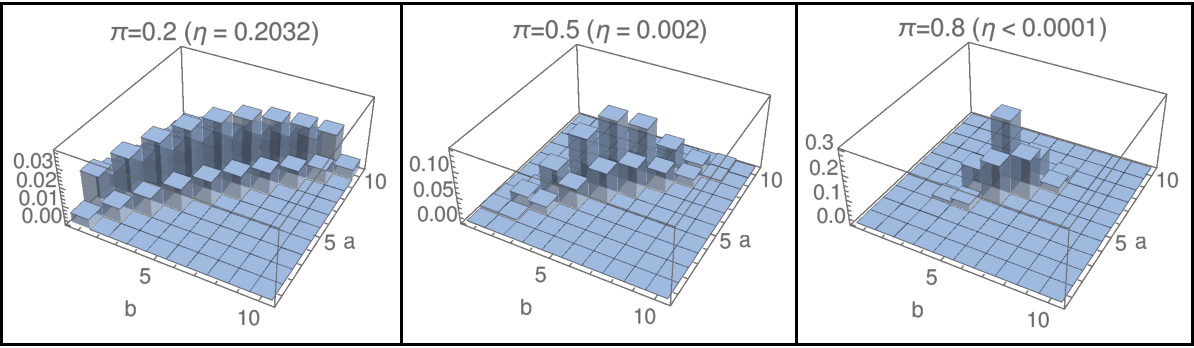
\includegraphics[width=\textwidth]{binom.pdf}
\caption{Distribution of $(A,B)$ in a call auction with $c=0$, $d = 11$, $D=\sum_{i=1}^{d-1} \delta_i V_i$, 
$S=\sum_{i=1}^{d-1} \delta_i W_i$, $V_i \sim \mathrm{Bernoulli}(\pi)$, $W_i \sim \mathrm{Bernoulli}(\pi)$, $0 < i < d$, $\indep(V_1,W_1,V_2,\dots,W_{d-1})$, for various levels of $\pi$. Here, $\eta = \P[B = 0 \vee C = 11]$.}
\label{fig:bin}
\end{center}
\end{figure}


\section{Unit Order Volumes}
\label{sec:cru}

In this subsection, we keep assuming $D\indep S$ to be completely random, but study the special case of the $D$ and $S$ being diffuse (i.e. for any $x\in I$, $D\{x\}=0$, $S\{x\}=0$ w.p.1) and simple (the atoms' weight is always unit). Given these assumptions, by \cite{Kallenberg02}, Theorem 12.10, both $D$ and $S$ are (equivalent to simple) Poisson point processes. Note that, due to our assumption of a finite number of atoms, $D$ and $S$ are fully characterized by 
$\kappa(x)\defined \E K(x)$, $\lambda(x)\defined\E L(x)$, respectively, $x \in I$, with $\kappa(c+)<\infty,\lambda(d-) < \infty$. Let us also recall that we can represent $D=\sum_{i=1}^{N_D} \delta_{V_i}$ where ${N_D}\sim \Po(\kappa(c+))$, the c.d.f. of each $V_i$, $i\in \N$, is $F_D(\bullet)\defined 1-\kappa(\bullet)/\kappa(c+)$, with $\indep (N_D.V_1,V_2,\dots)$ and, similarly, $S=\sum_{i=1}^{N_S} \delta_{W_i}$ where ${N_S}\sim \Po(\lambda(d-))$, the c.d.f. of each $W_i$ is $F_S(\bullet)=\lambda(\bullet)/\lambda(d-)$, and $\indep (N_S.W_1,W_2,\dots)$. 

The following result is a direct consequence of Proposition \ref{th:general}:

\begin{proposition} If $D \indep S$ are (simple) diffuse Poisson, then, for any $c < b \leq a < d$ and $X \subset \N_0$,
\begin{multline}
\P[B<b,A>a,V\in X]=\P[ D[b,a] = 0 ]\P[ S[b,a] = 0]\P[D(a,d)=S(c,b)\in X]\\
= e^{-(\lambda(a)-\lambda(b))}e^{-(\kappa(b)-\kappa(a))}\P[D(a,d)=S(c,b)\in X].
\label{eq:pax}
\end{multline}
\end{proposition}

Applying (\ref{eq:pax}) to single-element $X$'s, we get:
\begin{corollary} For any $c < b \leq a < d$, and $i \in \N_0$,
\begin{multline}
\P[B<b,A>a,V = i] = p(b,a,\{i\}) \\ \defined e^{-(\lambda(a)-\lambda(b))}e^{-(\kappa(b)-\kappa(a))} e^{-\kappa(a)} \frac{\kappa(a)^i}{i!}e^{-\lambda(b)} \frac{\lambda(b)^i}{i!}
 = e^{-\kappa(b)-\lambda(a)} \frac{\kappa(a)^i}{i!}\frac{\lambda(b)^i}{i!}.
\label{eq:pbai}
\end{multline}
\end{corollary}
Further, by taking $X = \N_0$ and using the fact that, for any $\mu\geq 0$ and $\nu \geq 0$, $\P[\Po(\mu)\stackrel{\indep{}}{-}\Po(\nu)=0]=e^{-\mu-\nu}I_{0}(2\sqrt{\mu\nu})$ where $I_0$ is the zero-order modified Bessel function of the first kind (see e.g. \cite{skellam1946frequency}), we get:
\begin{corollary} For any $c < b\leq a < c$,
\begin{equation}
\P[B<b,A>a]=p(b,a,\N_0) \defined e^{-\kappa(b)-\lambda(a)} I_{0}(2\sqrt{\kappa(a)\lambda(b)}).
\label{eq:pba}
\end{equation}
\end{corollary}
\begin{remark}
Equivalently, we can sum (\ref{eq:pbai}) to get,
$$
p(b,a,\N_0)=e^{-\kappa(b)-\lambda(a)}\sum_{i=0}^\infty\frac{(\kappa(a)\lambda(b))^i}{i!i!}.
$$
\end{remark}
As $\P[B\geq A]=0$, (\ref{eq:pbai}) and (\ref{eq:pba}) suffice to evaluate the distributions of $(A,B,V)$, $(A,B)$, respectively.

Assume, until the end of this Section, that $\kappa$ and $\lambda$ are differentiable.

\begin{proposition}
\label{th:abv}
Let either $X = \N_0$ or $X = \{i\}$ for some $i\in \N_0$. Then, for any $Q\in\B([c,d)\times(c,d])$,
\begin{multline}
\P[(B,A,V)\in Q \times X]=\int_{\{(b,a)\in Q: c<b<a<d\}}\gamma(b,a,X)dadb\\
+\charf [0\in X] \left[\int_{\{a:(c,a) \in Q \}}\alpha(a)da
+\int_{\{b:(b,d) \in Q \}}\beta(b)db+\charf[(c,d)\in Q]e^{-\kappa(c)-\lambda(d)}
\right],
\label{eq:pbc}
\end{multline}
where 
$$
\alpha(a)\defined 
\lambda'(a)e^{-\kappa(c)-\lambda(a)},\qquad
\beta(b)\defined-\kappa'(b)e^{-\kappa(b)}{}^{-\lambda(d)},
$$
and
$$
\gamma(b,a,X) = -\frac{\partial}{\partial a\partial b}p(b,a,X).
$$
\end{proposition}

\begin{proof}
See Appendix \ref{app:abv}.
\end{proof}

\begin{corollary}\label{cor:abdens} For any $Q\in\B([c,d)\times(c,d])$,
\begin{multline*}
\P[(B,A)\in Q]=\int_{\{(b,a)\in Q, b \in I, a \in I\}}g(b,a)dadb\\
+\int_{\{a:(c,a) \in Q \}}\alpha(a)da
+\int_{\{b:(b,d) \in Q \}}\beta(b)db+\charf[(c,d)\in Q]e^{-\kappa(c)-\lambda(d)}
\end{multline*}
where 
$$g(b,a)=0,\qquad a<b, $$
and
\begin{multline}
g(b,a)
%= e^{-\kappa(b)-\lambda(a)}
%\left(
%-\kappa'(b)\lambda'(a) \sum_{i=0}^\infty \frac{\lambda(b)^i\kappa(a)^i}{i!i!}
%+\kappa'(a)\kappa'(b) \sum_{i=0}^\infty \frac{\lambda(b)^{i+1}\kappa(a)^i}{(i+1)!i!}
%\right.
%\\
%\left.
%+\lambda'(b)\lambda'(a) \sum_{i=0}^\infty \frac{\lambda(b)^{i}\kappa(a)^{i+1}}{(i+1)!i!}
%-\lambda'(b)\kappa'(a) \sum_{i=0}^\infty \frac{\lambda(b)^{i}\kappa(a)^{i}}{i!i!}
%\right)\\
= e^{-\kappa(b)-\lambda(a)}
\left(
-\left[\kappa'(b)\lambda'(a)+\lambda'(b)\kappa'(a)\right] I_0(2\sqrt{\kappa(a)\lambda(b)})
\right.
\\
\left.
+\left[\kappa'(a)\kappa'(b)
\sqrt{\frac{\lambda(b)}{\kappa(a)}}
+\lambda'(a)\lambda'(b)
\sqrt{\frac{\kappa(a)}{\lambda(b)}}\right] I_1(2\sqrt{\kappa(a)\lambda(b)})
\right), \qquad a \geq b,
\label{eq:gamma}
\end{multline}
where $I_k$ is the modified Bessel function of $k$ -th order of the first kind; we take $\kappa'(a)\sqrt{\frac{\lambda(b)}{\kappa(a)}}=0$ whenever $\kappa(a)=0$ and 
$\lambda'(b)
\sqrt{\frac{\kappa(a)}{\lambda(b)}}=0$ whenever $\lambda(b)=0$.
\end{corollary}



\begin{proof} See Appendix \ref{app:abdens}.
\end{proof}

Furthermore, we evaluate the distribution of $(P,V)$:

\begin{proposition}
Let $X \subseteq \N_0$ be as in Proposition \ref{th:abv}. Then, 
\begin{equation}
\P[P=\undef, V\in X]=\charf[0\in X] [e^{-\kappa(c)}+e^{-\lambda(d)}-e^{-\kappa(c)-\lambda(d)}]\label{eq:pd0}
\end{equation}
and, for any $p\in I$,
\begin{multline}
\P[P<p,P\neq\undef,V\in X]\\=
%\Phi_{\kappa,\lambda}(p)\defined
\int_{c}^{p}\eta(a,a,X)da+\int_{p}^{(2p-c) \wedge d}\eta(2p-a,a,X)da+\charf[0 \in X] [e^{-\kappa(c)-\lambda((2p-c) \wedge d)}-e^{-\kappa(c)}]
\label{eq:pdist}
\end{multline}
where $\eta(b,a,X)=-\frac{\partial}{\partial a} p(b,a,X)$, $b<a$. 
\end{proposition}

\begin{proof}
By Proposition \ref{th:abv}, 
\begin{multline*}
\P[P<p,P\neq\undef,V\in X] =\P[A<d,c<B<2p-A,V\in X]
\\ =\int_{\{a < d\}}\int_{\{ c < b < 2p-a\}}\P_{(B,A,V)}(db,da,X)\\
=\int_{\{c< a < d\}}\int_{\underbrace{\{ c < b < 2p-a, b < a \}}_{\text{$=\emptyset$ for $a \geq 2p-c$}}}\gamma(b,a,X)dbda\\
=\int_c^{(2p-c) \wedge d}\int_c^{a \wedge (2p-a)} \gamma(b,a,X)dbda \\
=\int_c^{(2p-c) \wedge d}[ \eta(a \wedge 2p-a,a,X)da - \eta(c,a,X)]da\\
=\underbrace{\int_c^{(2p-c) \wedge d} \eta(a \wedge 2p-a,a,X)da}_
{=\int_c^p \eta(a, {\dots} + \int_p^{(2p-c) \wedge d} \eta(2p-a,\dots} +
\underbrace{\left[p(c,(2p-c) \wedge d,X)-p(c,c,X)\right]}_{=\charf[0\in X](e^{-\kappa(c)-\lambda((2p-c) \wedge d)}-e^{-\kappa(c)})}
\end{multline*}
(see Appendix \ref{app:abv} for the definition of $p(c,\bullet,X)$).
\end{proof}

\begin{theorem}
(i)
$$
\P[P=\undef]=e^{-\kappa(c)}+e^{-\lambda(d)}-e^{-\kappa(c)-\lambda(d)}.
$$

\noindent (ii) For any $p\in I$ and $v \in \N_0$,
\begin{multline}
\P[P<p,P\neq\undef,V = v]=
%\Phi_{\kappa,\lambda}(p)\defined
\int_{c}^{p}\psi(a,a,v)da \\ +\int_{p}^{(2p-c) \wedge d}\psi(2p-a,a,v)da+\charf[v=0] (e^{-\kappa(c)-\lambda((2p-c) \wedge d)}-e^{-\kappa(c)}),
\label{eq:pdist2}
\end{multline}
where
$$
\psi(b,a,v)=
\begin{cases}
e^{-\kappa(b)-\lambda(a)}\lambda'(a) & v=0,\\
e^{-\kappa(b)-\lambda(a)}\frac{\lambda(b)^v}{v!}\left(\lambda'(a)\frac{\kappa(a)^v}{v!}
- \kappa'(a)\frac{\kappa(a)^{v-1}}{{(v-1)}!}\right) & v>0.
\end{cases}
$$
\noindent (iii) For any $p \in I$,
\begin{multline}
\P[P<p,P\neq\undef]\\=
%\Phi_{\kappa,\lambda}(p)\defined
\int_{c}^{p}\phi(a,a)da+\int_{p}^{2p \wedge d}\phi(2p-a,a)da + [e^{-\kappa(c)-\lambda(2p \wedge d)}-e^{\kappa(c)}],
\label{eq:ppu}
\end{multline}
where 
$$
\phi(b,a)=
e^{-\kappa(b)-\lambda(a)}\left(-\lambda'(a)I_0(2\sqrt{\kappa(a)\lambda(b)})+\kappa'(a)\sqrt{\frac{\lambda(b)}{\kappa(a)}}I_1(2\sqrt{\kappa(a)\lambda(b)})\right)
$$
taking $\kappa'(a)\sqrt{\frac{\lambda(b)}{\kappa(a)}}=0$ whenever $\kappa(a)=0$.

\noindent (iv) For any $v\in \N_0$,
$$
\P[V=v]\\=
%\Phi_{\kappa,\lambda}(p)\defined
\int_{c}^{d}\psi(a,a,v)da + \charf[v = 0] e^{-\lambda(d)}.
$$
\end{theorem}

\begin{proof} (i) follows from (\ref{eq:pd0}), (ii) and (iii) follow from (\ref{eq:pdist}), to get (iv), it suffices to take the limit $p\rightarrow d$ in (\ref{eq:pdist}).
\end{proof}

\begin{corollary} \label{cor:dens}
 $P$ is absolutely continuous w.r.t. $\delta_\undef+\ell((c,d))$, where $\ell$ denotes the Lebesgue measure, with density 
\begin{equation}
f(\undef)=e^{-\kappa(c)}+e^{-\lambda(d)}-e^{-\kappa(c)-\lambda(d)},\qquad 
f(p)=2 \int_p^{2 p \wedge d} g(2p-a,a) da.
\label{eq:pdens}
\end{equation}
\end{corollary}

\begin{proof} See Appendix \ref{app:dens}.
\end{proof}




 

\section{Random Order Volumes}
\label{sec:crr}

In the present Section, we release the assumption of unit weights, still assuming that $D\indep S$ are diffuse complete random, but allowing for (i.i.d.) random weights with the same distribution for buy-- and the sell orders. Under these assumptions, the locations of the $D$'s and $S$'s atoms form a (diffuse) Poisson point processes, which we denote $D_g$, $S_g$, respectively.

\def\cpo{\mathrm{CPo}}

\begin{theorem} Let $D \indep S$, let $D_g$, $S_g$ be diffuse Poisson and let the weights of the atoms be i.i.d., following a distribution $\L$ such that $\L(-\infty,0]=0$. Then, for any $c < b \leq a < d$,
\begin{equation}
\label{eq:pbcp}
\P[B<b] = \P[\mathcal{C}(\kappa_g(b),\lambda_g(b),\L)\leq 0],
\end{equation}
\begin{equation}
\label{eq:pacp}
\P[A<a] = \P[\mathcal{C}(\kappa_g(a),\lambda_g(a),\L)< 0],
\end{equation}
and
\begin{multline*}
\P[B<b,A<a] = \P[\mathcal{C}(\kappa_g(b),\lambda_g(b),\L)\leq 0]
\\
- e^{-(\lambda_g(a)-\lambda_g(b))}e^{-(\kappa_g(b)-\kappa_g(a))}\P[\mathcal{C}(\kappa_g(a),\lambda_g(b),\L)=0];
\end{multline*}
here, $\kappa_g(\pi)=\E D_g[\pi,d)$, $\lambda_g(\pi)=\E S_g(c,\pi]$, $\pi \in I$, and $\mathcal{C}(\kappa,\lambda,\L)$ is the Compound Poisson distribution with intensity $\kappa+\lambda$ and embedded distribution $\frac\kappa{\kappa+\lambda} \L + \frac\lambda{\kappa+\lambda} \L^-$ where $\L^-$ is  the $\L$'s negative version (i.e. $\L(x,\infty)=\L^-(-\infty,-x)$, $x \in \R$).
\end{theorem}
\begin{proof}
The assertion follows from Proposition \ref{cor:cr}, using the fact that the convolution of two compound Poisson distributions is compound Poison with properly weighted mixed embedded distribution.
\end{proof}

%https://www.sciencedirect.com/science/article/abs/pii/0167637784900087

\noindent In the following Theorem, we evaluate the asymptotic distributions of the clearing price and the bounds of the traded volume.

\begin{theorem} \label{th:asymp} Let $\kappa_0,\lambda_0:I\rightarrow \R_+$ be strictly increasing, decreasing, respectively, and differentiable. Let $\L$ be distribution with $\L(-\infty,0]=0$ having a finite third moment. For any $n \in \N$, let $P_n,B_n,A_n,\dots$ be the clearing price, lower price limit, upper price limit, etc., in a call auction with independent compound Poisson order books defined by $\kappa_g = n \kappa_0$ and $\lambda_g = n\lambda_0$ and the atoms' weight distribution $\L$. Let $p$ be the solution of the equation $\kappa_0(p)= \lambda_0(p)$. Then\\
(i) $$P_n\stackrel{P}\longrightarrow p$$
(ii)
\begin{multline*}
\sqrt{n}(P_n-p) \stackrel{d} \longrightarrow \ND\left(0,v_gr_\L\right), 
\\ 
v_g \defined \frac{\kappa_0(p)+\lambda_0(p)}{(\lambda_0'(p)-\kappa_0'(p))^2}=\frac{2\kappa_0(p)}{(\lambda_0'(p)-\kappa_0'(p))^2}
=
\frac{2\lambda_0(p)}{(\lambda_0'(p)-\kappa_0'(p))^2},
\qquad
r_\L = \frac{\E \L^2}{(\E \L)^2},
\end{multline*}
where  $\E\L$ and $\E\L^2$ are the $\L$'s expectation, (non-central) second moment, respectively.\\
(iii) 
$$W^-_n \leq V_n \leq W^+_n,\qquad 
W^-_n \defined V_n^-(p),\qquad W_n^+ \defined V_n^+(p),$$
with
$$
\frac{1}{\sqrt{n}}(W_n^--n \mu)\stackrel{d}\longrightarrow \mathcal{M}_{w}, 
\qquad 
\frac{1}{\sqrt{n}}(W_n^+-n \mu)\stackrel{d}\longrightarrow \mathcal{M}^{w};
$$
$$
\mu = \kappa_0(p) \E\L = \lambda_0(p) \E\L, \quad
w = 
\kappa_0(p) \E \L^2= \lambda_0(p) \E \L^2,
$$
where $\mathcal{M}_w$, $\mathcal{M}^w$, are the distributions of the minimum, maximum, respectively, of two independent $\ND(0,w)$ random variables. In particular
$$
\P\left[ \frac{1}{\sqrt{n}}(W^-_n-n \mu)  < x
\right] = 1-\left(1-\varphi\left(\frac{x}{\sqrt{w}}\right) \right)^2,
$$
$$
\P\left[ \frac{1}{\sqrt{n}}(W^+_n-n \mu) < x
\right] = \varphi\left(\frac{x}{\sqrt{w}}\right)^2,
$$
where $\varphi$ is the standard normal c.d.f.
\end{theorem}

\begin{proof} See Appendix \ref{app:asymp}.
\end{proof}


\begin{corollary}
If, in Theorem \ref{th:asymp}, $\L = \delta_1$ (i.e., the volumes are deterministic and unit), then the Theorem holds with 
$v_g = \frac{2\kappa(p)}{[\lambda'(p)-\kappa'(p)]^2}$, $r_L=1$, $\mu = w = \kappa(p)=\lambda(p)$.
\end{corollary}

\paragraph*{Numerical Illustration.}
Once the trading intensities are high enough, we can represent $P=P_n$, $V^-(p)=V_n^-(p)$ and $V^+(p)=V_n^+(p)$ for some $n$ and approximate
$$
P \quad \dot \sim \quad 
\ND\left(p,\frac{2\kappa_g(p)\E\L^2}{(\kappa'_g(p)-\lambda'_g(p))^2(\E \L)^2} \right ),
$$
and
$$
W^- \leq V \leq W^+,
$$
where
$$
\P\left[ W^-  < x
\right] \doteq 1-\left(1-\varphi\left(\frac{\kappa_g(p)\E \L+x}{\sqrt{\kappa_g(p)\E \L^2}}\right) \right)^2
$$
$$
\P\left[ W^+ < x
\right] \doteq \varphi\left(\frac{\kappa_g(p)\E \L+x}{\sqrt{\kappa_g(p)\E \L^2}}\right)^2
$$
$x \in I$. In Figure \ref{fig:il}, we illustrate the accuracy of these approximations for various levels of trading intensity: we assume that order volumes and intensities are multiples of linear functions, different for demand and supply. It can be seen that the approximations are nearly perfect, once there are tens of orders on both sides (recall that the expected number of buy and sell orders equals $\kappa(c+)$, $\lambda(d-)$, respectively.

\begin{remark} As, by the Schwarz inequality, $r_\L \geq 1$, with the minimum achieved by $\L = \delta_1$, we see that taking randomness of the order volumes into account leads to higher (asymptotic) variance of both the price and the volume bounds in comparison with the usual approximation of the volumes by their mean values (normed to one). 
\end{remark}

Next, we compare our asymptotic result with that of \cite{derksen2020clearing}:

\begin{remark} Consider
$$
D=\sum_{i=1}^{N_D} \delta_{D_i}, \qquad S=\sum_{i=1}^{N_S} \delta_{S_i}
$$
where $\E N_D=(1-\alpha)n$, $\E N_S=\alpha n$ for some $\alpha \in (0,1)$ and $n\in \N$,  $D_i$, $i\in\N$, being i.i.d. with strictly increasing absolutely continuous c.d.f. $F_D$, and $S_i$, $i\in \N$ being i.i.d. with strictly increasing a.c. c.d.f $F_S$, such that all the variables are mutually independent.

Once $N_S$ and $N_D$ are Poisson, $D$ and $S$ are Poisson processes determined by 
$$
\kappa(x)=n (1-\alpha) (1-F_D(x)), \qquad \lambda(x)=n \alpha F_S(x),
$$
and, by Theorem \ref{th:asymp},
$$
\sqrt{n}(P_n-p) \rightarrow_n \ND(0,v), 
\qquad 
v=\frac{ 2 \alpha F_S(p) }{[(1-\alpha)f_D(p)+\alpha f_S(p)]^2}.
$$
 

If, instead, $N_D=(1-\alpha) n$ and $N_S = \alpha n$ are deterministic, we have, by Theorem 3.1 of \cite{derksen2020clearing}, that 
$$
\sqrt{n}(P_n-p) \rightarrow_n \ND(0,\tilde v), 
\qquad 
\tilde v=\frac{ \alpha [F_D(p)+ (1-F_S(p))]F_S(p)}{[(1-\alpha)f_D(p)+\alpha f_S(p)]^2}
$$
By comparison of the asymptotic variances we see that assuming random order numbers increases the price variance significantly compared with only using their expectations. 
\end{remark}


\begin{figure}
\begin{center}
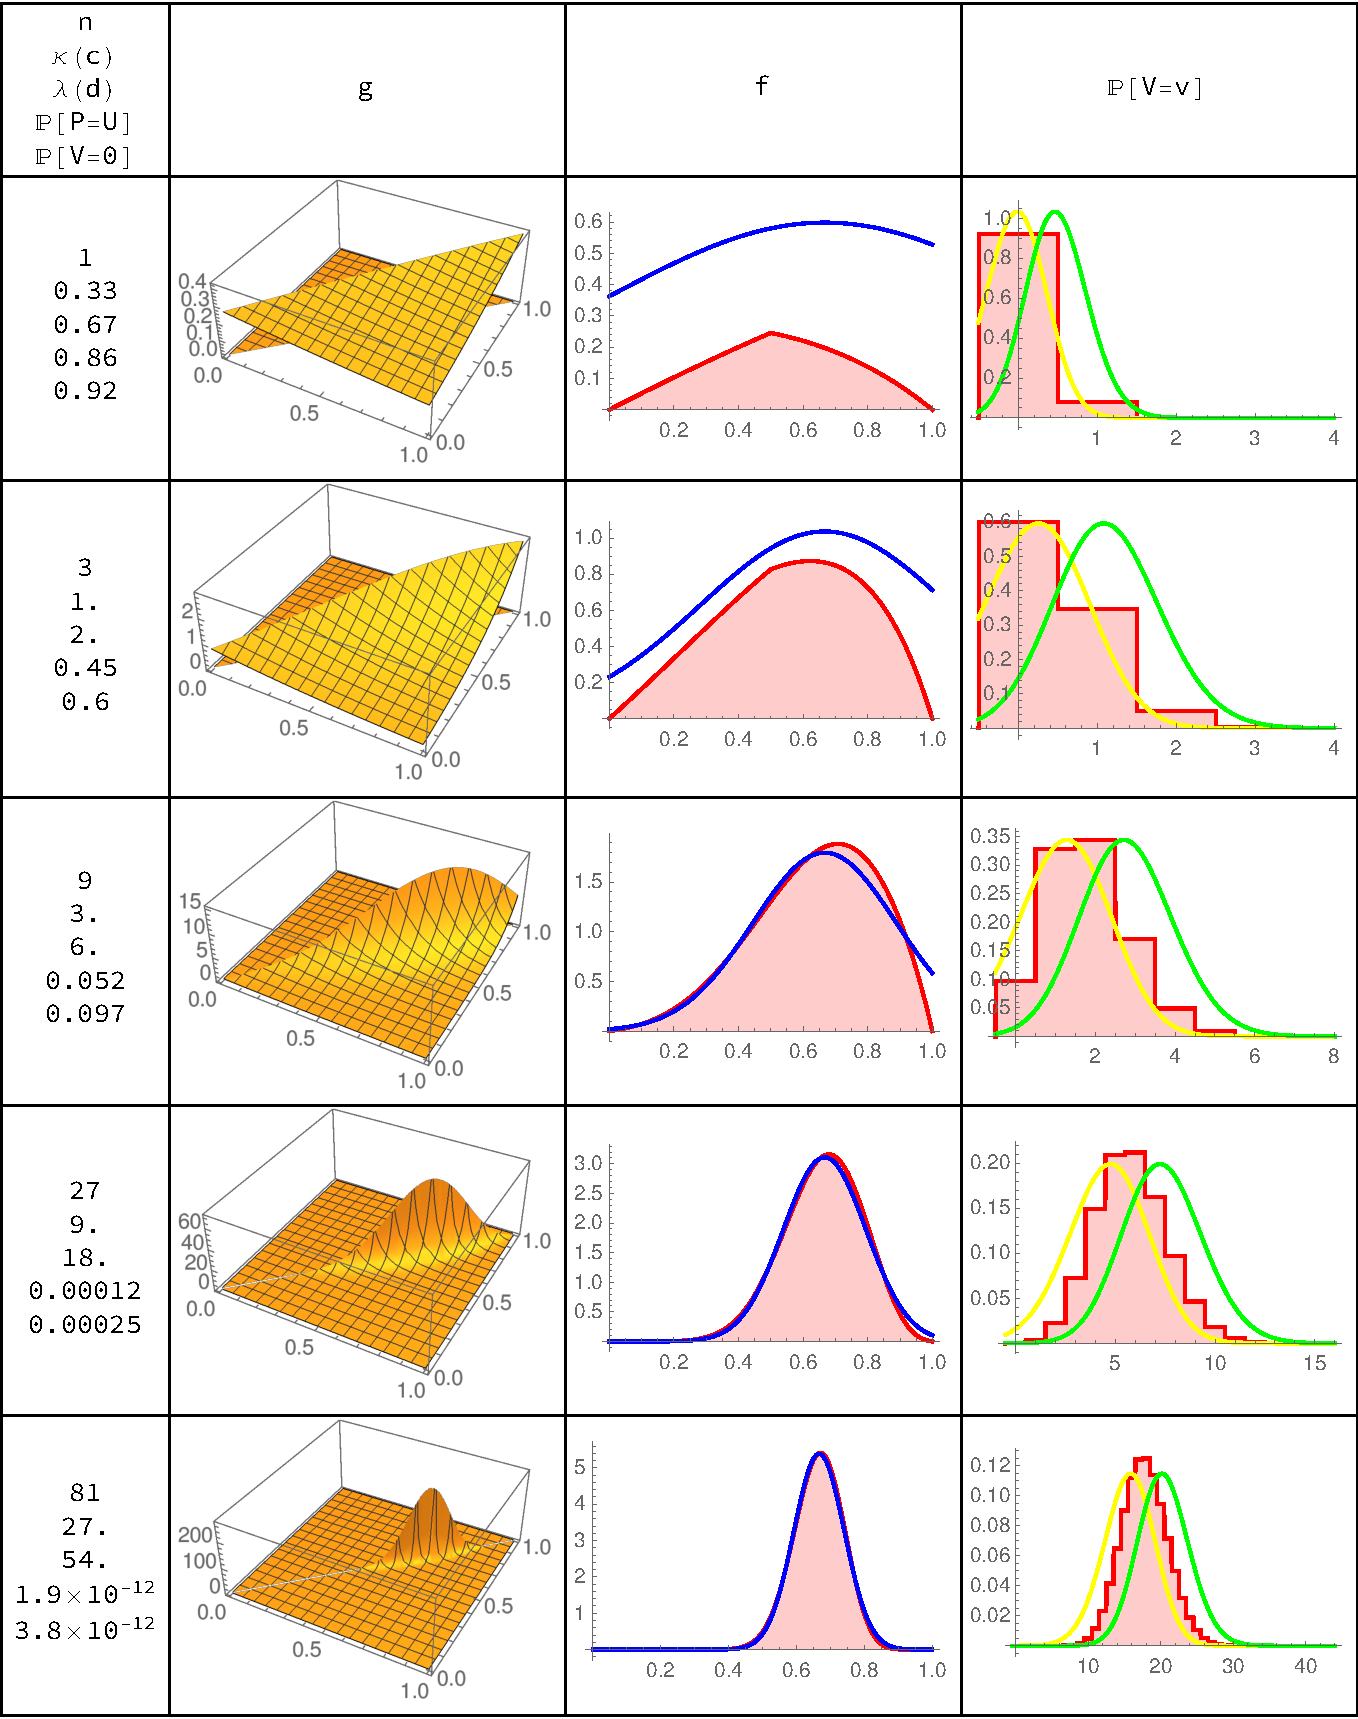
\includegraphics[width=\textwidth]{illust.pdf}
\caption{Distribution of $(A,B)$, $P$ and $V$ for $\kappa(a)=n \frac{2}{3}(1-a)$, $\lambda(b)=n \frac{1}3 b$ and unit order volumes. Blue, normal approximation of $P$, yellow, normal approximation of $W^-$, green, normal approximation of $W^+$. }
\label{fig:il}
\end{center}
\end{figure}

\section{Conclusions}

We have thoroughly studied a natural stochastic model of call auction. We have described both the exact and the asymptotic distributions in various special cases of this model. The next natural step could be to describe the dynamics of repeated call auctions, suggested by \cite{budish2015high}, and compare it with that of the continuous double auction.

\paragraph*{Acknowledgments} This work was supported by grant No. GA19-11062S from the Czech Science Foundation. Computational resources were partially provided by the ``eInfrastruktura CZ'' (e-INFRA CZ LM2018140) project supported by the Ministry of Education, Youth and
Sports of the Czech Republic

%\bibliographystyle{APT}
\footnotesize
%\bibliography{../../smid}
\input{call.bbl}
\appendix



\section{Proofs}

\subsection{Proof of Proposition \ref{th:abv}}
\label{app:abv}


Denote $Z \defined [c,d)\times(c,d]$. 
By taking the limits in (\ref{eq:pax}), we get the following.
\begin{multline}
p(c,a,X)\defined\P[B=c,A>a,V\in X]=
\lim_{b\downarrow c} p(b,a,X) \\
=e^{-(\lambda(a)-\lambda(c+))}e^{-(\kappa(c+)-\kappa(a))}
\underbrace{\P[D[a,d)=0\in X]}_{=\exp\{-(\kappa(d)-\kappa(a))\}\charf[0 \in X]}=e^{-\kappa(c)-\lambda(a)}\charf[0 \in X]
\label{eq:pca}
\end{multline}
because $\kappa$ is continuous and $\kappa(d)=\lambda(c+)=0$. Similarly we get
$$
p(b,d,X)\defined\P[B <b,A=d,V \in X]=p(b,d-,X) = e^{-\kappa(b)-\lambda(d)}\charf[0 \in X],
$$
and
\[
p(c,d,X)\defined\P[B=c,A=d,V \in X]=p(c+,d-,X)´=e^{-\kappa(c)-\lambda(d)}\charf[0 \in X].
\]

Agree to extend $p$ to $Z$ by taking limits as above and note that $\frac\partial{\partial a}p$, $\frac\partial{\partial b}p$ and $\frac\partial{\partial b\partial a}p$ exist on the interior of $Z$.

Denote $H\defined\{(y,z)\in Z:y<x\}$ and, for any $Q\in \B(Z)$, denote $$\varpi_X(Q)\defined\P[(B,A,V)\in Q \times X].$$

For any $(b,a)\in Z$, put $Q_{b,a}\defined[c,b)\times(a,d]$. Applying (\ref{eq:pax}), its extensions and the differentiability of $p$, we get that, for any $(b,a)\in H$,
\begin{multline*}
\varpi_X(Q_{b,a})=p(b,a,X)=p(b,d,X)-\int_{a}^{d}\frac{\partial}{\partial x}p(b,x,X)dx\\
=p(c,d,X)+\int_{c}^{b}\frac{\partial}{\partial y}p(y,d,X)dy-\int_{a}^{d}\left(\frac{\partial}{\partial x}p(c,x,X)+\int_{c}^{b}\frac{\partial}{\partial x\delta y}p(y,x,X)dy\right)dx,
\end{multline*}
which gives (\ref{eq:pbc}) for $Q=Q_{b,a}$ whenever $(b,a)\in H$.

As $\varpi_X$ is a measure on $(Z,\B(Z))$, we get, by elementary set operations,
that (\ref{eq:pbc}) holds for any $Q_{n}\defined\bigcup_{i=-n2^{n}}^{n2^{n}}Q_{\frac{i}{2^{n}},\frac{i+1}{2^{n}}}$,
$n\in\N$, and consequently for any 
$Q_{n,y,z}\defined Q_{n}\cap Q_{y,z}$, $(y,z)\in Z$, $n\in\N$.

Now let $(b,a)\in Z\setminus H.$  As $Q_{1}\subset Q_{2}\subset\dots$
and $\bigcup_{n}Q_{n}=H,$ we further have
\begin{multline*}
\varpi_X Q_{b,a}\stackrel{\P[Z\setminus H]=0}{=}\varpi_X(Q_{b,a}\cap H)
=\varpi_X(Q_{b,a}\cap \bigcup_n Q_n)
\\
=\varpi_X(\bigcup_n Q_{n,b,a})
=\lim_{n}\varpi_X Q_{n,b,a}
=\varpi_X(\cup_{n}Q_{n,b,a})=\varpi_X(Q_{b,a}).
\end{multline*}
As $(Q_{b,a})_{(b.a)\in Z}$ generate $\B(Z)$ and $\varpi_X$ is bounded, we are getting
(\ref{eq:pbc}) by \cite{Kallenberg02}, Lemma 1.17.


\subsection{Proof of Corollary \ref{cor:abdens}}
\label{app:abdens}

It suffices to show that $\gamma(a,b,\N_0)=g(a,b)$ for any $a \geq b$: Agreeing to write $I_k$ instead of $I_k (2\sqrt{\kappa(a)\lambda(b)}$, $k=1,2$, and differentiating (see \cite{wolframbessel}), we get
\begin{multline*} 
\gamma(y,x,\N_0)=-\frac{\partial}{\partial a \partial b } p(b,a,\N_0)=
-\kappa'(b)e^{-\kappa(b)-\lambda(a)}\left(\lambda'(a)I_{0}-\kappa'(a)\sqrt{\frac{\lambda(b)}{\kappa(a)}}I{}_{1}\right)\\+e^{-\kappa(b)-\lambda(a)}
\left(\lambda'(a)
\underbrace{\frac\partial{\partial b}I_{0}}
_{=\lambda'(b)\sqrt{\frac{\kappa(a)}{\lambda(b)}} I_{1}}
-
\kappa'(a)\lambda'(b)
\left[
I_1 
\underbrace{
\frac{\partial}{\partial b}\sqrt{\frac{\lambda(b)}{\kappa(a)}}
}
_
{
=\frac{1}{2\sqrt{\kappa(a)\lambda(b)}}
}
+
\sqrt{\frac{\lambda(b)}{\kappa(a)}} 
\underbrace{
\frac{\partial}{\partial b} I_{1}
}_
{=[I_{0}-\frac1{2\sqrt{\kappa(b)\lambda(a)}}I_{1}]
\sqrt{\frac{\kappa(a)}{\lambda(b)}}}
\right]\right).
\end{multline*}
Putting this together, we get (\ref{eq:gamma}).
%\begin{multline}
%e^{-\kappa(b)-\lambda(a)}\left(-\left[\kappa'(b)\lambda'(a)+\kappa'(a)\lambda'(b)\right]I_{0}\right.
%\\
%\left.
%+\left[\kappa'(b)\kappa'(a)\sqrt{\frac{\lambda(b)}{\kappa(a)}}
%+\lambda'(b)\lambda'(a)\sqrt{\frac{\kappa(a)}{\lambda(b)}}\right]I_1
%\right)
%ˇ\end{multline}

%To evaluate $\gamma$, we get
%\begin{multline*}
%-\frac{\partial}{\partial a \partial b}p(b,a,\{i\})
%=
%-\frac{\partial}{\partial a \partial b}\left(e^{-\kappa(b)-\lambda(a)} \frac{\kappa(a)^i}{i!}\frac{\lambda(b)^i}{i!}\right)
%\\
%= e^{-\kappa(b)-\lambda(a)}
%\left(
%-\kappa'(b)\frac{\lambda(b)^i}{i!}
%+\lambda'(b)\frac{\lambda(b)^{i-1}}{(i-1)!}
%\right)
%\left(\lambda'(a)\frac{\kappa(a)^i}{i!}
%- \kappa'(a)\frac{\kappa(a)^{i-1}}{{(i-1)}!}\right)
%\end{multline*}
%and
%$$
%-\frac{\partial}{\partial a \partial b}p(b,a,\{0\})
%=-\kappa'(b)\lambda'(a)e^{-\kappa(b)-\lambda(a)}
%$$
%By summing, we get 



\subsection{Proof of Corollary \ref{cor:dens}}
\label{app:dens}


The Dirac part of (\ref{eq:pdens}) is obvious. The Lebesgue part can be obtained by  differentiating (\ref{eq:ppu}):
\begin{multline}
f(p) = \phi(p,p)+\charf[2p-c < d]2 \underbrace{\phi(c,2p-c)}_{\stackrel{(\ref{eq:pca})}=\lambda'(2p-c)e^{-\kappa(c)-\lambda(2p-c)}}-\phi(p,p)
\\+
\int_c^{(2p-c)\wedge d}\frac{\partial}{\partial p}\phi(2p-a,a)da
-\charf[2p-c < d]2\lambda'(2p-c)e^{-\kappa(c)-\lambda(2p-c)}
\\
=2\int_c^{(2p-c)\wedge d}\gamma(2p-a,a)da
\end{multline}

\subsection{Proof of Theorem \ref{th:asymp}}
\label{app:asymp}

\begin{lemma}\label{lem:pois}
Let $Y_n \sim \cpo(n\lambda_n,\mathcal{D})$ 
where $\E \mathcal{D}^3 < \infty$ and $\lambda_n \rightarrow \lambda$ for some $\lambda > 0$. Then
$$
\frac{S_n}{s_n} \stackrel{d}\longrightarrow \ND(0,1), \qquad S_n=Y_n - n\lambda_n \E \mathcal{D},\quad s_n = \sqrt{n \lambda_n \E \mathcal{D}^2}.
$$
\end{lemma}

\begin{proof} Denote $\mu_i$, $\nu_i$, the $i$-th central, non-central moment, respectively, of $\mathcal{D}$ and note that we can represent 
$$
S_n = \sum_{i=1}^n (X_{i,n}-\lambda_n\nu_1),\qquad X_{i,n} \sim \mathcal\cpo(\lambda_n,\mathcal{D}),
$$
so the Lemma holds by the Lyapunov Central Limit Theorem for triangular arrays,
%perhaps Lehman sec 2.7
 provided that the Lyapunov Condition holds: By the Law of Total Cummulance, for any $S
=\sum_{i=1}^N Z_i \sim \cpo(\lambda,\mathcal{D})$, we have, 
\begin{multline*}
\E (S-\E S)^3= \E(\E((S-\E(S|N))^3|N)) + \E(\E(S|N)-\E(S))^3+3\cov(\E(S|N),\var(S|N))
\\=\E(N \mu_3)+\E(N \nu_1 - \lambda \nu_1 )^3+3\cov(N\nu_1,N\mu_2)
= \mu_3 \lambda + \nu^3_1 \lambda + \nu_1 \mu_2 \lambda
\end{multline*}
(see \cite{kendall1948advanced}, (5.20), for the third moment of Poisson distribution), so the Lyapunov conidition holds:
$$
\frac{1}{s^3_n} \sum_{i=1}^n (X_{i,n}-\lambda_n\nu_1)^3=\frac{n\lambda_n (\mu_3+\nu_1^3+\nu_1\mu_2)}{n^{3/2}\lambda^{3/2}_n \nu_2^{3/2}}\stackrel{n}\longrightarrow 0.
$$

\end{proof}

\noindent {\bf Proof of the Theorem.} Ad
(ii). By Theorem \ref{th:gen}, we have, for any $x\in I$, 
$$
[\sqrt{n}(A_n - p) < x] = [A_n < p + \frac x{\sqrt{n}}] = [ (N_n)_{p+\frac{x}{\sqrt n}} < 0]= [M_n < 0]
$$
$$
M_n
=\frac{1}{\sqrt{n\nu}}[D_n[p+\frac{x}{\sqrt{n}},d)-S_n(c,p+\frac{x}{\sqrt{n}})]
=U_n - V_n + W_n
$$
where $\nu=\kappa_0(p) \E \L^2=\lambda_0(p) \E \L^2$,
$$
U_n =\frac{1}{\sqrt{n\nu}}\left[D_n[p+\frac{x}{\sqrt{n}},d)-n \kappa(p+\frac{x}{\sqrt{n}})\right]
,\qquad
\kappa=\kappa_0 \E \L,
$$
$$
V_n =\frac{1}{\sqrt{n\nu}}\left[S_n(c,p+\frac{x}{\sqrt{n}})-n \lambda(p+\frac{x}{\sqrt{n}})\right],
\qquad \lambda = \lambda_0\E\L,
$$
and
$$
W_n =\frac{1}{\sqrt{n\nu}}\left[n\kappa(p+\frac{x}{\sqrt{n}})-n\lambda(p+\frac{x}{\sqrt{n}})\right]
={\sqrt{\frac n\nu}}\left[
(\kappa(p+\frac{x}{\sqrt{n}})-\kappa(p))-(\lambda(p+\frac{x}{\sqrt{n}})-\lambda(p))
\right]
$$
(recall that $\kappa(p)=\lambda(p)$). Further,
$$
U_n =\underbrace{\underbrace{\sqrt{\frac{\kappa_0(p+\frac{x}{\sqrt{n}}) \E \L^2}\nu}}
_{\longrightarrow 1} 
\cdot \underbrace{\frac{D_n[p+\frac{x}{\sqrt{n}},d)-n \kappa(p+\frac{x}{\sqrt{n}})}{\sqrt{n\kappa_0(p+\frac{x}{\sqrt{n}}) \E \L^2}}}_{\longrightarrow_d \ND(0,1)}}_{\longrightarrow_d \ND(0,1)}
$$
where the right-hand factor converges by Lemma \ref{lem:pois} while the product converges by Cramer-Slutsky Theorem. Similarly we get that 
$
V_n \rightarrow \ND(0,1)
$.

Further,
$$
W_n = {\sqrt{\frac n\nu}}\left[
\kappa'(p)\frac{x}{\sqrt{n}}-\lambda'(p)\frac{x}{\sqrt{n}}
+o\left(\frac 1{\sqrt{n}}\right)\right]\longrightarrow \frac{\kappa'(p)-\lambda'(p)}{\sqrt{\nu}}x
$$

Finally, by the Continuous Mapping Theorem and the fact that $U_n,V_n,W_n$ are independent, we get that $$M_n \rightarrow \ND(\frac{\kappa'(p)-\lambda'(p)}{\sqrt{\nu}}x,2),$$
so
$$
\P[\sqrt{n}(A_n - p) < x] \rightarrow \P[\ND(\frac{\kappa'(p)-\lambda'(p)}{\sqrt{\nu}}x,2)<0]
=\P[\ND(0,v_g r_\L)<x].
$$
By the same procedure we get that 
$$
\P[\sqrt{n}(B_n - p) < x] \rightarrow \P[\ND(\frac{\kappa'(p)-\lambda'(p)}{\sqrt{\nu}}x,2)<0]
=\P[\ND(0,v_g r_\L)<x].
$$
As $P_n \neq \undef \Rightarrow B_n \leq P_n \leq A_n$ and as $\P[P_n=\undef] \leq \P[D_n=0 \vee S_n=0] \leq \P[D_n=0] + \P[S_n=0] \rightarrow 0$, we get (ii).\\
(i) follows from (ii) by \cite{Kallenberg02}, Lemma 4.7. \\
(iii) By Lemma \ref{lem:pois}, $$U_n \defined \frac{1}{\sqrt{n}}(K_n(p)-n\mu) \stackrel{d}  \rightarrow \ND(0,w)$$ and $$V_n \defined \frac{1}{\sqrt{n}}(L_n(p)-n\mu) \stackrel{d}  \rightarrow \ND(0,w),$$ so
$$
\frac{1}{\sqrt{n}}(V^-_n(p)-n\mu)=\min(U_n,V_n) \stackrel{d} 
 \rightarrow \M_{w},
$$
by the Continuous Mapping Theorem. Similarly for $V_n^+$.

\end{document}

\begin{prop}
\label{prop:price}Let $D,S$ be independent Poisson
point processes,\footnote{Note that we implicitly assume the ordered/offered volumes to be unit.} put
$\kappa(\pi)=\E D[\pi,d),$ and $\lambda(\pi)=\E S(c,\pi]$ for any
$\pi\in[c,d].$ Let $\kappa,\lambda$ be differentiable bounded strictly
monotonous with bounded derivatives on C. Then
\begin{equation}
\P[P=\undef]=p_{\kappa,\lambda}\defined e^{-\kappa(c)}+e^{-\lambda(d)}-e^{-\kappa(c)-\lambda(d)}\label{eq:pd0}
\end{equation}
and
\begin{multline*}
\P[P<\pi,P\neq\undef]=\Phi_{\kappa,\lambda}(\pi)\defined\int_{c}^{\pi}\phi(a,a)da+\int_{\pi}^{d}\phi(2\pi-a,a)da-e^{-\kappa(c)}{}^{-\lambda(\pi)},\\
\phi(b,a)=e^{-\kappa(b)-\lambda(a)}\left(\lambda'(a)I_{0}(2\sqrt{\kappa(a)\lambda(b)})-\kappa'(a)\sqrt{\frac{\lambda(b)}{\kappa(a)}}I{}_{1}(2\sqrt{\kappa(a)\lambda(b)})\right),
\end{multline*}
where $I_k$ is the modified Bessel function of the first order $k$.
\end{prop}


\end{document}
From the definitions,
\begin{multline*}
\P[P=\undef]=\P[B=c\vee A=d]=\P[B=c]+\P[A=d]-\P[B=c,A=d]\\
=\P[DC=0]+\P[SC=0]-\P[DC=0]\P[SC=0],
\end{multline*}
which proves (\ref{eq:pd0}).

\appendix



\section{Proofs}

\subsection{Proof of Proposition \ref{th:abv}}
\label{app:abv}


Denote $Z \defined [c,d)\times(c,d]$. 
By taking the limits in (\ref{eq:pax}), we get the following.
\begin{multline}
p(c,a,X)\defined\P[B=c,A>a,V\in X]=
\lim_{b\downarrow c} p(b,a,X) \\
=e^{-(\lambda(a)-\lambda(c+))}e^{-(\kappa(c+)-\kappa(a))}
\underbrace{\P[D[a,d)=0\in X]}_{=\exp\{-(\kappa(d)-\kappa(a))\}\charf[0 \in X]}=e^{-\kappa(c)-\lambda(a)}\charf[0 \in X]
\label{eq:pca}
\end{multline}
because $\kappa$ is continuous and $\kappa(d)=\lambda(c+)=0$. Similarly we get
$$
p(b,d,X)\defined\P[B <b,A=d,V \in X]=p(b,d-,X) = e^{-\kappa(b)-\lambda(d)}\charf[0 \in X],
$$
and
\[
p(c,d,X)\defined\P[B=c,A=d,V \in X]=p(c+,d-,X)´=e^{-\kappa(c)-\lambda(d)}\charf[0 \in X].
\]

Agree to extend $p$ to $Z$ by taking limits as above and note that $\frac\partial{\partial a}p$, $\frac\partial{\partial b}p$ and $\frac\partial{\partial b\partial a}p$ exist on the interior of $Z$.

Denote $H\defined\{(y,z)\in Z:y<x\}$ and, for any $Q\in \B(Z)$, denote $$\varpi_X(Q)\defined\P[(B,A,V)\in Q \times X].$$

For any $(b,a)\in Z$, put $Q_{b,a}\defined[c,b)\times(a,d]$. Applying (\ref{eq:pax}), its extensions and the differentiability of $p$, we get that, for any $(b,a)\in H$,
\begin{multline*}
\varpi_X(Q_{b,a})=p(b,a,X)=p(b,d,X)-\int_{a}^{d}\frac{\partial}{\partial x}p(b,x,X)dx\\
=p(c,d,X)+\int_{c}^{b}\frac{\partial}{\partial y}p(y,d,X)dy-\int_{a}^{d}\left(\frac{\partial}{\partial x}p(c,x,X)+\int_{c}^{b}\frac{\partial}{\partial x\delta y}p(y,x,X)dy\right)dx,
\end{multline*}
which gives (\ref{eq:pbc}) for $Q=Q_{b,a}$ whenever $(b,a)\in H$.

As $\varpi_X$ is a measure on $(Z,\B(Z))$, we get, by elementary set operations,
that (\ref{eq:pbc}) holds for any $Q_{n}\defined\bigcup_{i=-n2^{n}}^{n2^{n}}Q_{\frac{i}{2^{n}},\frac{i+1}{2^{n}}}$,
$n\in\N$, and consequently for any 
$Q_{n,y,z}\defined Q_{n}\cap Q_{y,z}$, $(y,z)\in Z$, $n\in\N$.

Now let $(b,a)\in Z\setminus H.$  As $Q_{1}\subset Q_{2}\subset\dots$
and $\bigcup_{n}Q_{n}=H,$ we further have
\begin{multline*}
\varpi_X Q_{b,a}\stackrel{\P[Z\setminus H]=0}{=}\varpi_X(Q_{b,a}\cap H)
=\varpi_X(Q_{b,a}\cap \bigcup_n Q_n)
\\
=\varpi_X(\bigcup_n Q_{n,b,a})
=\lim_{n}\varpi_X Q_{n,b,a}
=\varpi_X(\cup_{n}Q_{n,b,a})=\varpi_X(Q_{b,a}).
\end{multline*}
As $(Q_{b,a})_{(b.a)\in Z}$ generate $\B(Z)$ and $\varpi_X$ is bounded, we are getting
(\ref{eq:pbc}) by \cite{Kallenberg02}, Lemma 1.17.


\subsection{Proof of Corollary \ref{cor:abdens}}
\label{app:abdens}

It suffices to show that $\gamma(a,b,\N_0)=g(a,b)$ for any $a \geq b$: Agreeing to write $I_k$ instead of $I_k (2\sqrt{\kappa(a)\lambda(b)}$, $k=1,2$, and differentiating (see \cite{wolframbessel}), we get
\begin{multline*} 
\gamma(y,x,\N_0)=-\frac{\partial}{\partial a \partial b } p(b,a,\N_0)=
-\kappa'(b)e^{-\kappa(b)-\lambda(a)}\left(\lambda'(a)I_{0}-\kappa'(a)\sqrt{\frac{\lambda(b)}{\kappa(a)}}I{}_{1}\right)\\+e^{-\kappa(b)-\lambda(a)}
\left(\lambda'(a)
\underbrace{\frac\partial{\partial b}I_{0}}
_{=\lambda'(b)\sqrt{\frac{\kappa(a)}{\lambda(b)}} I_{1}}
-
\kappa'(a)\lambda'(b)
\left[
I_1 
\underbrace{
\frac{\partial}{\partial b}\sqrt{\frac{\lambda(b)}{\kappa(a)}}
}
_
{
=\frac{1}{2\sqrt{\kappa(a)\lambda(b)}}
}
+
\sqrt{\frac{\lambda(b)}{\kappa(a)}} 
\underbrace{
\frac{\partial}{\partial b} I_{1}
}_
{=[I_{0}-\frac1{2\sqrt{\kappa(b)\lambda(a)}}I_{1}]
\sqrt{\frac{\kappa(a)}{\lambda(b)}}}
\right]\right).
\end{multline*}
Putting this together, we get (\ref{eq:gamma}).
%\begin{multline}
%e^{-\kappa(b)-\lambda(a)}\left(-\left[\kappa'(b)\lambda'(a)+\kappa'(a)\lambda'(b)\right]I_{0}\right.
%\\
%\left.
%+\left[\kappa'(b)\kappa'(a)\sqrt{\frac{\lambda(b)}{\kappa(a)}}
%+\lambda'(b)\lambda'(a)\sqrt{\frac{\kappa(a)}{\lambda(b)}}\right]I_1
%\right)
%ˇ\end{multline}

%To evaluate $\gamma$, we get
%\begin{multline*}
%-\frac{\partial}{\partial a \partial b}p(b,a,\{i\})
%=
%-\frac{\partial}{\partial a \partial b}\left(e^{-\kappa(b)-\lambda(a)} \frac{\kappa(a)^i}{i!}\frac{\lambda(b)^i}{i!}\right)
%\\
%= e^{-\kappa(b)-\lambda(a)}
%\left(
%-\kappa'(b)\frac{\lambda(b)^i}{i!}
%+\lambda'(b)\frac{\lambda(b)^{i-1}}{(i-1)!}
%\right)
%\left(\lambda'(a)\frac{\kappa(a)^i}{i!}
%- \kappa'(a)\frac{\kappa(a)^{i-1}}{{(i-1)}!}\right)
%\end{multline*}
%and
%$$
%-\frac{\partial}{\partial a \partial b}p(b,a,\{0\})
%=-\kappa'(b)\lambda'(a)e^{-\kappa(b)-\lambda(a)}
%$$
%By summing, we get 



\subsection{Proof of Corollary \ref{cor:dens}}
\label{app:dens}


The Dirac part of (\ref{eq:pdens}) is obvious. The Lebesgue part can be obtained by  differentiating (\ref{eq:ppu}):
\begin{multline}
f(p) = \phi(p,p)+\charf[2p-c < d]2 \underbrace{\phi(c,2p-c)}_{\stackrel{(\ref{eq:pca})}=\lambda'(2p-c)e^{-\kappa(c)-\lambda(2p-c)}}-\phi(p,p)
\\+
\int_c^{(2p-c)\wedge d}\frac{\partial}{\partial p}\phi(2p-a,a)da
-\charf[2p-c < d]2\lambda'(2p-c)e^{-\kappa(c)-\lambda(2p-c)}
\\
=2\int_c^{(2p-c)\wedge d}\gamma(2p-a,a)da
\end{multline}

\subsection{Proof of Theorem \ref{th:asymp}}
\label{app:asymp}

\begin{lemma}\label{lem:pois}
Let $Y_n \sim \cpo(n\lambda_n,\mathcal{D})$ 
where $\E \mathcal{D}^3 < \infty$ and $\lambda_n \rightarrow \lambda$ for some $\lambda > 0$. Then
$$
\frac{S_n}{s_n} \stackrel{d}\longrightarrow \ND(0,1), \qquad S_n=Y_n - n\lambda_n \E \mathcal{D},\quad s_n = \sqrt{n \lambda_n \E \mathcal{D}^2}.
$$
\end{lemma}

\begin{proof} Denote $\mu_i$, $\nu_i$, the $i$-th central, non-central moment, respectively, of $\mathcal{D}$ and note that we can represent 
$$
S_n = \sum_{i=1}^n (X_{i,n}-\lambda_n\nu_1),\qquad X_{i,n} \sim \mathcal\cpo(\lambda_n,\mathcal{D}),
$$
so the Lemma holds by the Lyapunov Central Limit Theorem for triangular arrays,
%perhaps Lehman sec 2.7
 provided that the Lyapunov Condition holds: By the Law of Total Cummulance, for any $S
=\sum_{i=1}^N Z_i \sim \cpo(\lambda,\mathcal{D})$, we have, 
\begin{multline*}
\E (S-\E S)^3= \E(\E((S-\E(S|N))^3|N)) + \E(\E(S|N)-\E(S))^3+3\cov(\E(S|N),\var(S|N))
\\=\E(N \mu_3)+\E(N \nu_1 - \lambda \nu_1 )^3+3\cov(N\nu_1,N\mu_2)
= \mu_3 \lambda + \nu^3_1 \lambda + \nu_1 \mu_2 \lambda
\end{multline*}
(see \cite{kendall1948advanced}, (5.20), for the third moment of Poisson distribution), so the Lyapunov conidition holds:
$$
\frac{1}{s^3_n} \sum_{i=1}^n (X_{i,n}-\lambda_n\nu_1)^3=\frac{n\lambda_n (\mu_3+\nu_1^3+\nu_1\mu_2)}{n^{3/2}\lambda^{3/2}_n \nu_2^{3/2}}\stackrel{n}\longrightarrow 0.
$$

\end{proof}

\noindent {\bf Proof of the Theorem.} Ad
(ii). By Theorem \ref{th:gen}, we have, for any $x\in I$, 
$$
[\sqrt{n}(A_n - p) < x] = [A_n < p + \frac x{\sqrt{n}}] = [ (N_n)_{p+\frac{x}{\sqrt n}} < 0]= [M_n < 0]
$$
$$
M_n
=\frac{1}{\sqrt{n\nu}}[D_n[p+\frac{x}{\sqrt{n}},d)-S_n(c,p+\frac{x}{\sqrt{n}})]
=U_n - V_n + W_n
$$
where $\nu=\kappa_0(p) \E \L^2=\lambda_0(p) \E \L^2$,
$$
U_n =\frac{1}{\sqrt{n\nu}}\left[D_n[p+\frac{x}{\sqrt{n}},d)-n \kappa(p+\frac{x}{\sqrt{n}})\right]
,\qquad
\kappa=\kappa_0 \E \L,
$$
$$
V_n =\frac{1}{\sqrt{n\nu}}\left[S_n(c,p+\frac{x}{\sqrt{n}})-n \lambda(p+\frac{x}{\sqrt{n}})\right],
\qquad \lambda = \lambda_0\E\L,
$$
and
$$
W_n =\frac{1}{\sqrt{n\nu}}\left[n\kappa(p+\frac{x}{\sqrt{n}})-n\lambda(p+\frac{x}{\sqrt{n}})\right]
={\sqrt{\frac n\nu}}\left[
(\kappa(p+\frac{x}{\sqrt{n}})-\kappa(p))-(\lambda(p+\frac{x}{\sqrt{n}})-\lambda(p))
\right]
$$
(recall that $\kappa(p)=\lambda(p)$). Further,
$$
U_n =\underbrace{\underbrace{\sqrt{\frac{\kappa_0(p+\frac{x}{\sqrt{n}}) \E \L^2}\nu}}
_{\longrightarrow 1} 
\cdot \underbrace{\frac{D_n[p+\frac{x}{\sqrt{n}},d)-n \kappa(p+\frac{x}{\sqrt{n}})}{\sqrt{n\kappa_0(p+\frac{x}{\sqrt{n}}) \E \L^2}}}_{\longrightarrow_d \ND(0,1)}}_{\longrightarrow_d \ND(0,1)}
$$
where the right-hand factor converges by Lemma \ref{lem:pois} while the product converges by Cramer-Slutsky Theorem. Similarly we get that 
$
V_n \rightarrow \ND(0,1)
$.

Further,
$$
W_n = {\sqrt{\frac n\nu}}\left[
\kappa'(p)\frac{x}{\sqrt{n}}-\lambda'(p)\frac{x}{\sqrt{n}}
+o\left(\frac 1{\sqrt{n}}\right)\right]\longrightarrow \frac{\kappa'(p)-\lambda'(p)}{\sqrt{\nu}}x
$$

Finally, by the Continuous Mapping Theorem and the fact that $U_n,V_n,W_n$ are independent, we get that $$M_n \rightarrow \ND(\frac{\kappa'(p)-\lambda'(p)}{\sqrt{\nu}}x,2),$$
so
$$
\P[\sqrt{n}(A_n - p) < x] \rightarrow \P[\ND(\frac{\kappa'(p)-\lambda'(p)}{\sqrt{\nu}}x,2)<0]
=\P[\ND(0,v_g r_\L)<x].
$$
By the same procedure we get that 
$$
\P[\sqrt{n}(B_n - p) < x] \rightarrow \P[\ND(\frac{\kappa'(p)-\lambda'(p)}{\sqrt{\nu}}x,2)<0]
=\P[\ND(0,v_g r_\L)<x].
$$
As $P_n \neq \undef \Rightarrow B_n \leq P_n \leq A_n$ and as $\P[P_n=\undef] \leq \P[D_n=0 \vee S_n=0] \leq \P[D_n=0] + \P[S_n=0] \rightarrow 0$, we get (ii).\\
(i) follows from (ii) by \cite{Kallenberg02}, Lemma 4.7. \\
(iii) By Lemma \ref{lem:pois}, $$U_n \defined \frac{1}{\sqrt{n}}(K_n(p)-n\mu) \stackrel{d}  \rightarrow \ND(0,w)$$ and $$V_n \defined \frac{1}{\sqrt{n}}(L_n(p)-n\mu) \stackrel{d}  \rightarrow \ND(0,w),$$ so
$$
\frac{1}{\sqrt{n}}(V^-_n(p)-n\mu)=\min(U_n,V_n) \stackrel{d} 
 \rightarrow \M_{w},
$$
by the Continuous Mapping Theorem. Similarly for $V_n^+$.

\end{document}

\begin{prop}
\label{prop:price}Let $D,S$ be independent Poisson
point processes,\footnote{Note that we implicitly assume the ordered/offered volumes to be unit.} put
$\kappa(\pi)=\E D[\pi,d),$ and $\lambda(\pi)=\E S(c,\pi]$ for any
$\pi\in[c,d].$ Let $\kappa,\lambda$ be differentiable bounded strictly
monotonous with bounded derivatives on C. Then
\begin{equation}
\P[P=\undef]=p_{\kappa,\lambda}\defined e^{-\kappa(c)}+e^{-\lambda(d)}-e^{-\kappa(c)-\lambda(d)}\label{eq:pd0}
\end{equation}
and
\begin{multline*}
\P[P<\pi,P\neq\undef]=\Phi_{\kappa,\lambda}(\pi)\defined\int_{c}^{\pi}\phi(a,a)da+\int_{\pi}^{d}\phi(2\pi-a,a)da-e^{-\kappa(c)}{}^{-\lambda(\pi)},\\
\phi(b,a)=e^{-\kappa(b)-\lambda(a)}\left(\lambda'(a)I_{0}(2\sqrt{\kappa(a)\lambda(b)})-\kappa'(a)\sqrt{\frac{\lambda(b)}{\kappa(a)}}I{}_{1}(2\sqrt{\kappa(a)\lambda(b)})\right),
\end{multline*}
where $I_k$ is the modified Bessel function of the first order $k$.
\end{prop}


\end{document}
From the definitions,
\begin{multline*}
\P[P=\undef]=\P[B=c\vee A=d]=\P[B=c]+\P[A=d]-\P[B=c,A=d]\\
=\P[DC=0]+\P[SC=0]-\P[DC=0]\P[SC=0],
\end{multline*}
which proves (\ref{eq:pd0}).

\appendix



\section{Proofs}

\subsection{Proof of Proposition \ref{th:abv}}
\label{app:abv}


Denote $Z \defined [c,d)\times(c,d]$. 
By taking the limits in (\ref{eq:pax}), we get the following.
\begin{multline}
p(c,a,X)\defined\P[B=c,A>a,V\in X]=
\lim_{b\downarrow c} p(b,a,X) \\
=e^{-(\lambda(a)-\lambda(c+))}e^{-(\kappa(c+)-\kappa(a))}
\underbrace{\P[D[a,d)=0\in X]}_{=\exp\{-(\kappa(d)-\kappa(a))\}\charf[0 \in X]}=e^{-\kappa(c)-\lambda(a)}\charf[0 \in X]
\label{eq:pca}
\end{multline}
because $\kappa$ is continuous and $\kappa(d)=\lambda(c+)=0$. Similarly we get
$$
p(b,d,X)\defined\P[B <b,A=d,V \in X]=p(b,d-,X) = e^{-\kappa(b)-\lambda(d)}\charf[0 \in X],
$$
and
\[
p(c,d,X)\defined\P[B=c,A=d,V \in X]=p(c+,d-,X)´=e^{-\kappa(c)-\lambda(d)}\charf[0 \in X].
\]

Agree to extend $p$ to $Z$ by taking limits as above and note that $\frac\partial{\partial a}p$, $\frac\partial{\partial b}p$ and $\frac\partial{\partial b\partial a}p$ exist on the interior of $Z$.

Denote $H\defined\{(y,z)\in Z:y<x\}$ and, for any $Q\in \B(Z)$, denote $$\varpi_X(Q)\defined\P[(B,A,V)\in Q \times X].$$

For any $(b,a)\in Z$, put $Q_{b,a}\defined[c,b)\times(a,d]$. Applying (\ref{eq:pax}), its extensions and the differentiability of $p$, we get that, for any $(b,a)\in H$,
\begin{multline*}
\varpi_X(Q_{b,a})=p(b,a,X)=p(b,d,X)-\int_{a}^{d}\frac{\partial}{\partial x}p(b,x,X)dx\\
=p(c,d,X)+\int_{c}^{b}\frac{\partial}{\partial y}p(y,d,X)dy-\int_{a}^{d}\left(\frac{\partial}{\partial x}p(c,x,X)+\int_{c}^{b}\frac{\partial}{\partial x\delta y}p(y,x,X)dy\right)dx,
\end{multline*}
which gives (\ref{eq:pbc}) for $Q=Q_{b,a}$ whenever $(b,a)\in H$.

As $\varpi_X$ is a measure on $(Z,\B(Z))$, we get, by elementary set operations,
that (\ref{eq:pbc}) holds for any $Q_{n}\defined\bigcup_{i=-n2^{n}}^{n2^{n}}Q_{\frac{i}{2^{n}},\frac{i+1}{2^{n}}}$,
$n\in\N$, and consequently for any 
$Q_{n,y,z}\defined Q_{n}\cap Q_{y,z}$, $(y,z)\in Z$, $n\in\N$.

Now let $(b,a)\in Z\setminus H.$  As $Q_{1}\subset Q_{2}\subset\dots$
and $\bigcup_{n}Q_{n}=H,$ we further have
\begin{multline*}
\varpi_X Q_{b,a}\stackrel{\P[Z\setminus H]=0}{=}\varpi_X(Q_{b,a}\cap H)
=\varpi_X(Q_{b,a}\cap \bigcup_n Q_n)
\\
=\varpi_X(\bigcup_n Q_{n,b,a})
=\lim_{n}\varpi_X Q_{n,b,a}
=\varpi_X(\cup_{n}Q_{n,b,a})=\varpi_X(Q_{b,a}).
\end{multline*}
As $(Q_{b,a})_{(b.a)\in Z}$ generate $\B(Z)$ and $\varpi_X$ is bounded, we are getting
(\ref{eq:pbc}) by \cite{Kallenberg02}, Lemma 1.17.


\subsection{Proof of Corollary \ref{cor:abdens}}
\label{app:abdens}

It suffices to show that $\gamma(a,b,\N_0)=g(a,b)$ for any $a \geq b$: Agreeing to write $I_k$ instead of $I_k (2\sqrt{\kappa(a)\lambda(b)}$, $k=1,2$, and differentiating (see \cite{wolframbessel}), we get
\begin{multline*} 
\gamma(y,x,\N_0)=-\frac{\partial}{\partial a \partial b } p(b,a,\N_0)=
-\kappa'(b)e^{-\kappa(b)-\lambda(a)}\left(\lambda'(a)I_{0}-\kappa'(a)\sqrt{\frac{\lambda(b)}{\kappa(a)}}I{}_{1}\right)\\+e^{-\kappa(b)-\lambda(a)}
\left(\lambda'(a)
\underbrace{\frac\partial{\partial b}I_{0}}
_{=\lambda'(b)\sqrt{\frac{\kappa(a)}{\lambda(b)}} I_{1}}
-
\kappa'(a)\lambda'(b)
\left[
I_1 
\underbrace{
\frac{\partial}{\partial b}\sqrt{\frac{\lambda(b)}{\kappa(a)}}
}
_
{
=\frac{1}{2\sqrt{\kappa(a)\lambda(b)}}
}
+
\sqrt{\frac{\lambda(b)}{\kappa(a)}} 
\underbrace{
\frac{\partial}{\partial b} I_{1}
}_
{=[I_{0}-\frac1{2\sqrt{\kappa(b)\lambda(a)}}I_{1}]
\sqrt{\frac{\kappa(a)}{\lambda(b)}}}
\right]\right).
\end{multline*}
Putting this together, we get (\ref{eq:gamma}).
%\begin{multline}
%e^{-\kappa(b)-\lambda(a)}\left(-\left[\kappa'(b)\lambda'(a)+\kappa'(a)\lambda'(b)\right]I_{0}\right.
%\\
%\left.
%+\left[\kappa'(b)\kappa'(a)\sqrt{\frac{\lambda(b)}{\kappa(a)}}
%+\lambda'(b)\lambda'(a)\sqrt{\frac{\kappa(a)}{\lambda(b)}}\right]I_1
%\right)
%ˇ\end{multline}

%To evaluate $\gamma$, we get
%\begin{multline*}
%-\frac{\partial}{\partial a \partial b}p(b,a,\{i\})
%=
%-\frac{\partial}{\partial a \partial b}\left(e^{-\kappa(b)-\lambda(a)} \frac{\kappa(a)^i}{i!}\frac{\lambda(b)^i}{i!}\right)
%\\
%= e^{-\kappa(b)-\lambda(a)}
%\left(
%-\kappa'(b)\frac{\lambda(b)^i}{i!}
%+\lambda'(b)\frac{\lambda(b)^{i-1}}{(i-1)!}
%\right)
%\left(\lambda'(a)\frac{\kappa(a)^i}{i!}
%- \kappa'(a)\frac{\kappa(a)^{i-1}}{{(i-1)}!}\right)
%\end{multline*}
%and
%$$
%-\frac{\partial}{\partial a \partial b}p(b,a,\{0\})
%=-\kappa'(b)\lambda'(a)e^{-\kappa(b)-\lambda(a)}
%$$
%By summing, we get 



\subsection{Proof of Corollary \ref{cor:dens}}
\label{app:dens}


The Dirac part of (\ref{eq:pdens}) is obvious. The Lebesgue part can be obtained by  differentiating (\ref{eq:ppu}):
\begin{multline}
f(p) = \phi(p,p)+\charf[2p-c < d]2 \underbrace{\phi(c,2p-c)}_{\stackrel{(\ref{eq:pca})}=\lambda'(2p-c)e^{-\kappa(c)-\lambda(2p-c)}}-\phi(p,p)
\\+
\int_c^{(2p-c)\wedge d}\frac{\partial}{\partial p}\phi(2p-a,a)da
-\charf[2p-c < d]2\lambda'(2p-c)e^{-\kappa(c)-\lambda(2p-c)}
\\
=2\int_c^{(2p-c)\wedge d}\gamma(2p-a,a)da
\end{multline}

\subsection{Proof of Theorem \ref{th:asymp}}
\label{app:asymp}

\begin{lemma}\label{lem:pois}
Let $Y_n \sim \cpo(n\lambda_n,\mathcal{D})$ 
where $\E \mathcal{D}^3 < \infty$ and $\lambda_n \rightarrow \lambda$ for some $\lambda > 0$. Then
$$
\frac{S_n}{s_n} \stackrel{d}\longrightarrow \ND(0,1), \qquad S_n=Y_n - n\lambda_n \E \mathcal{D},\quad s_n = \sqrt{n \lambda_n \E \mathcal{D}^2}.
$$
\end{lemma}

\begin{proof} Denote $\mu_i$, $\nu_i$, the $i$-th central, non-central moment, respectively, of $\mathcal{D}$ and note that we can represent 
$$
S_n = \sum_{i=1}^n (X_{i,n}-\lambda_n\nu_1),\qquad X_{i,n} \sim \mathcal\cpo(\lambda_n,\mathcal{D}),
$$
so the Lemma holds by the Lyapunov Central Limit Theorem for triangular arrays,
%perhaps Lehman sec 2.7
 provided that the Lyapunov Condition holds: By the Law of Total Cummulance, for any $S
=\sum_{i=1}^N Z_i \sim \cpo(\lambda,\mathcal{D})$, we have, 
\begin{multline*}
\E (S-\E S)^3= \E(\E((S-\E(S|N))^3|N)) + \E(\E(S|N)-\E(S))^3+3\cov(\E(S|N),\var(S|N))
\\=\E(N \mu_3)+\E(N \nu_1 - \lambda \nu_1 )^3+3\cov(N\nu_1,N\mu_2)
= \mu_3 \lambda + \nu^3_1 \lambda + \nu_1 \mu_2 \lambda
\end{multline*}
(see \cite{kendall1948advanced}, (5.20), for the third moment of Poisson distribution), so the Lyapunov conidition holds:
$$
\frac{1}{s^3_n} \sum_{i=1}^n (X_{i,n}-\lambda_n\nu_1)^3=\frac{n\lambda_n (\mu_3+\nu_1^3+\nu_1\mu_2)}{n^{3/2}\lambda^{3/2}_n \nu_2^{3/2}}\stackrel{n}\longrightarrow 0.
$$

\end{proof}

\noindent {\bf Proof of the Theorem.} Ad
(ii). By Theorem \ref{th:gen}, we have, for any $x\in I$, 
$$
[\sqrt{n}(A_n - p) < x] = [A_n < p + \frac x{\sqrt{n}}] = [ (N_n)_{p+\frac{x}{\sqrt n}} < 0]= [M_n < 0]
$$
$$
M_n
=\frac{1}{\sqrt{n\nu}}[D_n[p+\frac{x}{\sqrt{n}},d)-S_n(c,p+\frac{x}{\sqrt{n}})]
=U_n - V_n + W_n
$$
where $\nu=\kappa_0(p) \E \L^2=\lambda_0(p) \E \L^2$,
$$
U_n =\frac{1}{\sqrt{n\nu}}\left[D_n[p+\frac{x}{\sqrt{n}},d)-n \kappa(p+\frac{x}{\sqrt{n}})\right]
,\qquad
\kappa=\kappa_0 \E \L,
$$
$$
V_n =\frac{1}{\sqrt{n\nu}}\left[S_n(c,p+\frac{x}{\sqrt{n}})-n \lambda(p+\frac{x}{\sqrt{n}})\right],
\qquad \lambda = \lambda_0\E\L,
$$
and
$$
W_n =\frac{1}{\sqrt{n\nu}}\left[n\kappa(p+\frac{x}{\sqrt{n}})-n\lambda(p+\frac{x}{\sqrt{n}})\right]
={\sqrt{\frac n\nu}}\left[
(\kappa(p+\frac{x}{\sqrt{n}})-\kappa(p))-(\lambda(p+\frac{x}{\sqrt{n}})-\lambda(p))
\right]
$$
(recall that $\kappa(p)=\lambda(p)$). Further,
$$
U_n =\underbrace{\underbrace{\sqrt{\frac{\kappa_0(p+\frac{x}{\sqrt{n}}) \E \L^2}\nu}}
_{\longrightarrow 1} 
\cdot \underbrace{\frac{D_n[p+\frac{x}{\sqrt{n}},d)-n \kappa(p+\frac{x}{\sqrt{n}})}{\sqrt{n\kappa_0(p+\frac{x}{\sqrt{n}}) \E \L^2}}}_{\longrightarrow_d \ND(0,1)}}_{\longrightarrow_d \ND(0,1)}
$$
where the right-hand factor converges by Lemma \ref{lem:pois} while the product converges by Cramer-Slutsky Theorem. Similarly we get that 
$
V_n \rightarrow \ND(0,1)
$.

Further,
$$
W_n = {\sqrt{\frac n\nu}}\left[
\kappa'(p)\frac{x}{\sqrt{n}}-\lambda'(p)\frac{x}{\sqrt{n}}
+o\left(\frac 1{\sqrt{n}}\right)\right]\longrightarrow \frac{\kappa'(p)-\lambda'(p)}{\sqrt{\nu}}x
$$

Finally, by the Continuous Mapping Theorem and the fact that $U_n,V_n,W_n$ are independent, we get that $$M_n \rightarrow \ND(\frac{\kappa'(p)-\lambda'(p)}{\sqrt{\nu}}x,2),$$
so
$$
\P[\sqrt{n}(A_n - p) < x] \rightarrow \P[\ND(\frac{\kappa'(p)-\lambda'(p)}{\sqrt{\nu}}x,2)<0]
=\P[\ND(0,v_g r_\L)<x].
$$
By the same procedure we get that 
$$
\P[\sqrt{n}(B_n - p) < x] \rightarrow \P[\ND(\frac{\kappa'(p)-\lambda'(p)}{\sqrt{\nu}}x,2)<0]
=\P[\ND(0,v_g r_\L)<x].
$$
As $P_n \neq \undef \Rightarrow B_n \leq P_n \leq A_n$ and as $\P[P_n=\undef] \leq \P[D_n=0 \vee S_n=0] \leq \P[D_n=0] + \P[S_n=0] \rightarrow 0$, we get (ii).\\
(i) follows from (ii) by \cite{Kallenberg02}, Lemma 4.7. \\
(iii) By Lemma \ref{lem:pois}, $$U_n \defined \frac{1}{\sqrt{n}}(K_n(p)-n\mu) \stackrel{d}  \rightarrow \ND(0,w)$$ and $$V_n \defined \frac{1}{\sqrt{n}}(L_n(p)-n\mu) \stackrel{d}  \rightarrow \ND(0,w),$$ so
$$
\frac{1}{\sqrt{n}}(V^-_n(p)-n\mu)=\min(U_n,V_n) \stackrel{d} 
 \rightarrow \M_{w},
$$
by the Continuous Mapping Theorem. Similarly for $V_n^+$.

\end{document}

\begin{prop}
\label{prop:price}Let $D,S$ be independent Poisson
point processes,\footnote{Note that we implicitly assume the ordered/offered volumes to be unit.} put
$\kappa(\pi)=\E D[\pi,d),$ and $\lambda(\pi)=\E S(c,\pi]$ for any
$\pi\in[c,d].$ Let $\kappa,\lambda$ be differentiable bounded strictly
monotonous with bounded derivatives on C. Then
\begin{equation}
\P[P=\undef]=p_{\kappa,\lambda}\defined e^{-\kappa(c)}+e^{-\lambda(d)}-e^{-\kappa(c)-\lambda(d)}\label{eq:pd0}
\end{equation}
and
\begin{multline*}
\P[P<\pi,P\neq\undef]=\Phi_{\kappa,\lambda}(\pi)\defined\int_{c}^{\pi}\phi(a,a)da+\int_{\pi}^{d}\phi(2\pi-a,a)da-e^{-\kappa(c)}{}^{-\lambda(\pi)},\\
\phi(b,a)=e^{-\kappa(b)-\lambda(a)}\left(\lambda'(a)I_{0}(2\sqrt{\kappa(a)\lambda(b)})-\kappa'(a)\sqrt{\frac{\lambda(b)}{\kappa(a)}}I{}_{1}(2\sqrt{\kappa(a)\lambda(b)})\right),
\end{multline*}
where $I_k$ is the modified Bessel function of the first order $k$.
\end{prop}


\end{document}
From the definitions,
\begin{multline*}
\P[P=\undef]=\P[B=c\vee A=d]=\P[B=c]+\P[A=d]-\P[B=c,A=d]\\
=\P[DC=0]+\P[SC=0]-\P[DC=0]\P[SC=0],
\end{multline*}
which proves (\ref{eq:pd0}).

\appendix



\section{Proofs}

\subsection{Proof of Proposition \ref{th:abv}}
\label{app:abv}


Denote $Z \defined [c,d)\times(c,d]$. 
By taking the limits in (\ref{eq:pax}), we get the following.
\begin{multline}
p(c,a,X)\defined\P[B=c,A>a,V\in X]=
\lim_{b\downarrow c} p(b,a,X) \\
=e^{-(\lambda(a)-\lambda(c+))}e^{-(\kappa(c+)-\kappa(a))}
\underbrace{\P[D[a,d)=0\in X]}_{=\exp\{-(\kappa(d)-\kappa(a))\}\charf[0 \in X]}=e^{-\kappa(c)-\lambda(a)}\charf[0 \in X]
\label{eq:pca}
\end{multline}
because $\kappa$ is continuous and $\kappa(d)=\lambda(c+)=0$. Similarly we get
$$
p(b,d,X)\defined\P[B <b,A=d,V \in X]=p(b,d-,X) = e^{-\kappa(b)-\lambda(d)}\charf[0 \in X],
$$
and
\[
p(c,d,X)\defined\P[B=c,A=d,V \in X]=p(c+,d-,X)´=e^{-\kappa(c)-\lambda(d)}\charf[0 \in X].
\]

Agree to extend $p$ to $Z$ by taking limits as above and note that $\frac\partial{\partial a}p$, $\frac\partial{\partial b}p$ and $\frac\partial{\partial b\partial a}p$ exist on the interior of $Z$.

Denote $H\defined\{(y,z)\in Z:y<x\}$ and, for any $Q\in \B(Z)$, denote $$\varpi_X(Q)\defined\P[(B,A,V)\in Q \times X].$$

For any $(b,a)\in Z$, put $Q_{b,a}\defined[c,b)\times(a,d]$. Applying (\ref{eq:pax}), its extensions and the differentiability of $p$, we get that, for any $(b,a)\in H$,
\begin{multline*}
\varpi_X(Q_{b,a})=p(b,a,X)=p(b,d,X)-\int_{a}^{d}\frac{\partial}{\partial x}p(b,x,X)dx\\
=p(c,d,X)+\int_{c}^{b}\frac{\partial}{\partial y}p(y,d,X)dy-\int_{a}^{d}\left(\frac{\partial}{\partial x}p(c,x,X)+\int_{c}^{b}\frac{\partial}{\partial x\delta y}p(y,x,X)dy\right)dx,
\end{multline*}
which gives (\ref{eq:pbc}) for $Q=Q_{b,a}$ whenever $(b,a)\in H$.

As $\varpi_X$ is a measure on $(Z,\B(Z))$, we get, by elementary set operations,
that (\ref{eq:pbc}) holds for any $Q_{n}\defined\bigcup_{i=-n2^{n}}^{n2^{n}}Q_{\frac{i}{2^{n}},\frac{i+1}{2^{n}}}$,
$n\in\N$, and consequently for any 
$Q_{n,y,z}\defined Q_{n}\cap Q_{y,z}$, $(y,z)\in Z$, $n\in\N$.

Now let $(b,a)\in Z\setminus H.$  As $Q_{1}\subset Q_{2}\subset\dots$
and $\bigcup_{n}Q_{n}=H,$ we further have
\begin{multline*}
\varpi_X Q_{b,a}\stackrel{\P[Z\setminus H]=0}{=}\varpi_X(Q_{b,a}\cap H)
=\varpi_X(Q_{b,a}\cap \bigcup_n Q_n)
\\
=\varpi_X(\bigcup_n Q_{n,b,a})
=\lim_{n}\varpi_X Q_{n,b,a}
=\varpi_X(\cup_{n}Q_{n,b,a})=\varpi_X(Q_{b,a}).
\end{multline*}
As $(Q_{b,a})_{(b.a)\in Z}$ generate $\B(Z)$ and $\varpi_X$ is bounded, we are getting
(\ref{eq:pbc}) by \cite{Kallenberg02}, Lemma 1.17.


\subsection{Proof of Corollary \ref{cor:abdens}}
\label{app:abdens}

It suffices to show that $\gamma(a,b,\N_0)=g(a,b)$ for any $a \geq b$: Agreeing to write $I_k$ instead of $I_k (2\sqrt{\kappa(a)\lambda(b)}$, $k=1,2$, and differentiating (see \cite{wolframbessel}), we get
\begin{multline*} 
\gamma(y,x,\N_0)=-\frac{\partial}{\partial a \partial b } p(b,a,\N_0)=
-\kappa'(b)e^{-\kappa(b)-\lambda(a)}\left(\lambda'(a)I_{0}-\kappa'(a)\sqrt{\frac{\lambda(b)}{\kappa(a)}}I{}_{1}\right)\\+e^{-\kappa(b)-\lambda(a)}
\left(\lambda'(a)
\underbrace{\frac\partial{\partial b}I_{0}}
_{=\lambda'(b)\sqrt{\frac{\kappa(a)}{\lambda(b)}} I_{1}}
-
\kappa'(a)\lambda'(b)
\left[
I_1 
\underbrace{
\frac{\partial}{\partial b}\sqrt{\frac{\lambda(b)}{\kappa(a)}}
}
_
{
=\frac{1}{2\sqrt{\kappa(a)\lambda(b)}}
}
+
\sqrt{\frac{\lambda(b)}{\kappa(a)}} 
\underbrace{
\frac{\partial}{\partial b} I_{1}
}_
{=[I_{0}-\frac1{2\sqrt{\kappa(b)\lambda(a)}}I_{1}]
\sqrt{\frac{\kappa(a)}{\lambda(b)}}}
\right]\right).
\end{multline*}
Putting this together, we get (\ref{eq:gamma}).
%\begin{multline}
%e^{-\kappa(b)-\lambda(a)}\left(-\left[\kappa'(b)\lambda'(a)+\kappa'(a)\lambda'(b)\right]I_{0}\right.
%\\
%\left.
%+\left[\kappa'(b)\kappa'(a)\sqrt{\frac{\lambda(b)}{\kappa(a)}}
%+\lambda'(b)\lambda'(a)\sqrt{\frac{\kappa(a)}{\lambda(b)}}\right]I_1
%\right)
%ˇ\end{multline}

%To evaluate $\gamma$, we get
%\begin{multline*}
%-\frac{\partial}{\partial a \partial b}p(b,a,\{i\})
%=
%-\frac{\partial}{\partial a \partial b}\left(e^{-\kappa(b)-\lambda(a)} \frac{\kappa(a)^i}{i!}\frac{\lambda(b)^i}{i!}\right)
%\\
%= e^{-\kappa(b)-\lambda(a)}
%\left(
%-\kappa'(b)\frac{\lambda(b)^i}{i!}
%+\lambda'(b)\frac{\lambda(b)^{i-1}}{(i-1)!}
%\right)
%\left(\lambda'(a)\frac{\kappa(a)^i}{i!}
%- \kappa'(a)\frac{\kappa(a)^{i-1}}{{(i-1)}!}\right)
%\end{multline*}
%and
%$$
%-\frac{\partial}{\partial a \partial b}p(b,a,\{0\})
%=-\kappa'(b)\lambda'(a)e^{-\kappa(b)-\lambda(a)}
%$$
%By summing, we get 



\subsection{Proof of Corollary \ref{cor:dens}}
\label{app:dens}


The Dirac part of (\ref{eq:pdens}) is obvious. The Lebesgue part can be obtained by  differentiating (\ref{eq:ppu}):
\begin{multline}
f(p) = \phi(p,p)+\charf[2p-c < d]2 \underbrace{\phi(c,2p-c)}_{\stackrel{(\ref{eq:pca})}=\lambda'(2p-c)e^{-\kappa(c)-\lambda(2p-c)}}-\phi(p,p)
\\+
\int_c^{(2p-c)\wedge d}\frac{\partial}{\partial p}\phi(2p-a,a)da
-\charf[2p-c < d]2\lambda'(2p-c)e^{-\kappa(c)-\lambda(2p-c)}
\\
=2\int_c^{(2p-c)\wedge d}\gamma(2p-a,a)da
\end{multline}

\subsection{Proof of Theorem \ref{th:asymp}}
\label{app:asymp}

\begin{lemma}\label{lem:pois}
Let $Y_n \sim \cpo(n\lambda_n,\mathcal{D})$ 
where $\E \mathcal{D}^3 < \infty$ and $\lambda_n \rightarrow \lambda$ for some $\lambda > 0$. Then
$$
\frac{S_n}{s_n} \stackrel{d}\longrightarrow \ND(0,1), \qquad S_n=Y_n - n\lambda_n \E \mathcal{D},\quad s_n = \sqrt{n \lambda_n \E \mathcal{D}^2}.
$$
\end{lemma}

\begin{proof} Denote $\mu_i$, $\nu_i$, the $i$-th central, non-central moment, respectively, of $\mathcal{D}$ and note that we can represent 
$$
S_n = \sum_{i=1}^n (X_{i,n}-\lambda_n\nu_1),\qquad X_{i,n} \sim \mathcal\cpo(\lambda_n,\mathcal{D}),
$$
so the Lemma holds by the Lyapunov Central Limit Theorem for triangular arrays,
%perhaps Lehman sec 2.7
 provided that the Lyapunov Condition holds: By the Law of Total Cummulance, for any $S
=\sum_{i=1}^N Z_i \sim \cpo(\lambda,\mathcal{D})$, we have, 
\begin{multline*}
\E (S-\E S)^3= \E(\E((S-\E(S|N))^3|N)) + \E(\E(S|N)-\E(S))^3+3\cov(\E(S|N),\var(S|N))
\\=\E(N \mu_3)+\E(N \nu_1 - \lambda \nu_1 )^3+3\cov(N\nu_1,N\mu_2)
= \mu_3 \lambda + \nu^3_1 \lambda + \nu_1 \mu_2 \lambda
\end{multline*}
(see \cite{kendall1948advanced}, (5.20), for the third moment of Poisson distribution), so the Lyapunov conidition holds:
$$
\frac{1}{s^3_n} \sum_{i=1}^n (X_{i,n}-\lambda_n\nu_1)^3=\frac{n\lambda_n (\mu_3+\nu_1^3+\nu_1\mu_2)}{n^{3/2}\lambda^{3/2}_n \nu_2^{3/2}}\stackrel{n}\longrightarrow 0.
$$

\end{proof}

\noindent {\bf Proof of the Theorem.} Ad
(ii). By Theorem \ref{th:gen}, we have, for any $x\in I$, 
$$
[\sqrt{n}(A_n - p) < x] = [A_n < p + \frac x{\sqrt{n}}] = [ (N_n)_{p+\frac{x}{\sqrt n}} < 0]= [M_n < 0]
$$
$$
M_n
=\frac{1}{\sqrt{n\nu}}[D_n[p+\frac{x}{\sqrt{n}},d)-S_n(c,p+\frac{x}{\sqrt{n}})]
=U_n - V_n + W_n
$$
where $\nu=\kappa_0(p) \E \L^2=\lambda_0(p) \E \L^2$,
$$
U_n =\frac{1}{\sqrt{n\nu}}\left[D_n[p+\frac{x}{\sqrt{n}},d)-n \kappa(p+\frac{x}{\sqrt{n}})\right]
,\qquad
\kappa=\kappa_0 \E \L,
$$
$$
V_n =\frac{1}{\sqrt{n\nu}}\left[S_n(c,p+\frac{x}{\sqrt{n}})-n \lambda(p+\frac{x}{\sqrt{n}})\right],
\qquad \lambda = \lambda_0\E\L,
$$
and
$$
W_n =\frac{1}{\sqrt{n\nu}}\left[n\kappa(p+\frac{x}{\sqrt{n}})-n\lambda(p+\frac{x}{\sqrt{n}})\right]
={\sqrt{\frac n\nu}}\left[
(\kappa(p+\frac{x}{\sqrt{n}})-\kappa(p))-(\lambda(p+\frac{x}{\sqrt{n}})-\lambda(p))
\right]
$$
(recall that $\kappa(p)=\lambda(p)$). Further,
$$
U_n =\underbrace{\underbrace{\sqrt{\frac{\kappa_0(p+\frac{x}{\sqrt{n}}) \E \L^2}\nu}}
_{\longrightarrow 1} 
\cdot \underbrace{\frac{D_n[p+\frac{x}{\sqrt{n}},d)-n \kappa(p+\frac{x}{\sqrt{n}})}{\sqrt{n\kappa_0(p+\frac{x}{\sqrt{n}}) \E \L^2}}}_{\longrightarrow_d \ND(0,1)}}_{\longrightarrow_d \ND(0,1)}
$$
where the right-hand factor converges by Lemma \ref{lem:pois} while the product converges by Cramer-Slutsky Theorem. Similarly we get that 
$
V_n \rightarrow \ND(0,1)
$.

Further,
$$
W_n = {\sqrt{\frac n\nu}}\left[
\kappa'(p)\frac{x}{\sqrt{n}}-\lambda'(p)\frac{x}{\sqrt{n}}
+o\left(\frac 1{\sqrt{n}}\right)\right]\longrightarrow \frac{\kappa'(p)-\lambda'(p)}{\sqrt{\nu}}x
$$

Finally, by the Continuous Mapping Theorem and the fact that $U_n,V_n,W_n$ are independent, we get that $$M_n \rightarrow \ND(\frac{\kappa'(p)-\lambda'(p)}{\sqrt{\nu}}x,2),$$
so
$$
\P[\sqrt{n}(A_n - p) < x] \rightarrow \P[\ND(\frac{\kappa'(p)-\lambda'(p)}{\sqrt{\nu}}x,2)<0]
=\P[\ND(0,v_g r_\L)<x].
$$
By the same procedure we get that 
$$
\P[\sqrt{n}(B_n - p) < x] \rightarrow \P[\ND(\frac{\kappa'(p)-\lambda'(p)}{\sqrt{\nu}}x,2)<0]
=\P[\ND(0,v_g r_\L)<x].
$$
As $P_n \neq \undef \Rightarrow B_n \leq P_n \leq A_n$ and as $\P[P_n=\undef] \leq \P[D_n=0 \vee S_n=0] \leq \P[D_n=0] + \P[S_n=0] \rightarrow 0$, we get (ii).\\
(i) follows from (ii) by \cite{Kallenberg02}, Lemma 4.7. \\
(iii) By Lemma \ref{lem:pois}, $$U_n \defined \frac{1}{\sqrt{n}}(K_n(p)-n\mu) \stackrel{d}  \rightarrow \ND(0,w)$$ and $$V_n \defined \frac{1}{\sqrt{n}}(L_n(p)-n\mu) \stackrel{d}  \rightarrow \ND(0,w),$$ so
$$
\frac{1}{\sqrt{n}}(V^-_n(p)-n\mu)=\min(U_n,V_n) \stackrel{d} 
 \rightarrow \M_{w},
$$
by the Continuous Mapping Theorem. Similarly for $V_n^+$.

\end{document}

\begin{prop}
\label{prop:price}Let $D,S$ be independent Poisson
point processes,\footnote{Note that we implicitly assume the ordered/offered volumes to be unit.} put
$\kappa(\pi)=\E D[\pi,d),$ and $\lambda(\pi)=\E S(c,\pi]$ for any
$\pi\in[c,d].$ Let $\kappa,\lambda$ be differentiable bounded strictly
monotonous with bounded derivatives on C. Then
\begin{equation}
\P[P=\undef]=p_{\kappa,\lambda}\defined e^{-\kappa(c)}+e^{-\lambda(d)}-e^{-\kappa(c)-\lambda(d)}\label{eq:pd0}
\end{equation}
and
\begin{multline*}
\P[P<\pi,P\neq\undef]=\Phi_{\kappa,\lambda}(\pi)\defined\int_{c}^{\pi}\phi(a,a)da+\int_{\pi}^{d}\phi(2\pi-a,a)da-e^{-\kappa(c)}{}^{-\lambda(\pi)},\\
\phi(b,a)=e^{-\kappa(b)-\lambda(a)}\left(\lambda'(a)I_{0}(2\sqrt{\kappa(a)\lambda(b)})-\kappa'(a)\sqrt{\frac{\lambda(b)}{\kappa(a)}}I{}_{1}(2\sqrt{\kappa(a)\lambda(b)})\right),
\end{multline*}
where $I_k$ is the modified Bessel function of the first order $k$.
\end{prop}


\end{document}
From the definitions,
\begin{multline*}
\P[P=\undef]=\P[B=c\vee A=d]=\P[B=c]+\P[A=d]-\P[B=c,A=d]\\
=\P[DC=0]+\P[SC=0]-\P[DC=0]\P[SC=0],
\end{multline*}
which proves (\ref{eq:pd0}).
